\documentclass{beamer}

% xcolor and define colors -------------------------
\usepackage{xcolor}

% https://www.viget.com/articles/color-contrast/
\definecolor{purple}{HTML}{5601A4}
\definecolor{navy}{HTML}{0D3D56}
\definecolor{ruby}{HTML}{9a2515}
\definecolor{alice}{HTML}{107895}
\definecolor{daisy}{HTML}{EBC944}
\definecolor{coral}{HTML}{F26D21}
\definecolor{kelly}{HTML}{829356}
\definecolor{cranberry}{HTML}{E64173}
\definecolor{jet}{HTML}{131516}
\definecolor{asher}{HTML}{555F61}
\definecolor{slate}{HTML}{314F4F}

% Mixtape Sessions
\definecolor{picton-blue}{HTML}{00b7ff}
\definecolor{violet-red}{HTML}{ff3881}
\definecolor{sun}{HTML}{ffaf18}
\definecolor{electric-violet}{HTML}{871EFF}

% Main theme colors
\definecolor{accent}{HTML}{00b7ff}
\definecolor{accent2}{HTML}{871EFF}
\definecolor{gray100}{HTML}{f3f4f6}
\definecolor{gray800}{HTML}{1F292D}


% Beamer Options -------------------------------------

% Background
\setbeamercolor{background canvas}{bg = white}

% Change text margins
\setbeamersize{text margin left = 15pt, text margin right = 15pt} 

% \alert
\setbeamercolor{alerted text}{fg = accent2}

% Frame title
\setbeamercolor{frametitle}{bg = white, fg = jet}
\setbeamercolor{framesubtitle}{bg = white, fg = accent}
\setbeamerfont{framesubtitle}{size = \small, shape = \itshape}

% Block
\setbeamercolor{block title}{fg = white, bg = accent2}
\setbeamercolor{block body}{fg = gray800, bg = gray100}

% Title page
\setbeamercolor{title}{fg = gray800}
\setbeamercolor{subtitle}{fg = accent}

%% Custom \maketitle and \titlepage
\setbeamertemplate{title page}
{
    %\begin{centering}
        \vspace{20mm}
        {\Large \usebeamerfont{title}\usebeamercolor[fg]{title}\inserttitle}\\
        {\large \itshape \usebeamerfont{subtitle}\usebeamercolor[fg]{subtitle}\insertsubtitle}\\ \vspace{10mm}
        {\insertauthor}\\
        {\color{asher}\small{\insertdate}}\\
    %\end{centering}
}

% Table of Contents
\setbeamercolor{section in toc}{fg = accent!70!jet}
\setbeamercolor{subsection in toc}{fg = jet}

% Button 
\setbeamercolor{button}{bg = accent}

% Remove navigation symbols
\setbeamertemplate{navigation symbols}{}

% Table and Figure captions
\setbeamercolor{caption}{fg=jet!70!white}
\setbeamercolor{caption name}{fg=jet}
\setbeamerfont{caption name}{shape = \itshape}

% Bullet points

%% Fix left-margins
\settowidth{\leftmargini}{\usebeamertemplate{itemize item}}
\addtolength{\leftmargini}{\labelsep}

%% enumerate item color
\setbeamercolor{enumerate item}{fg = accent}
\setbeamerfont{enumerate item}{size = \small}
\setbeamertemplate{enumerate item}{\insertenumlabel.}

%% itemize
\setbeamercolor{itemize item}{fg = accent!70!white}
\setbeamerfont{itemize item}{size = \small}
\setbeamertemplate{itemize item}[circle]

%% right arrow for subitems
\setbeamercolor{itemize subitem}{fg = accent!60!white}
\setbeamerfont{itemize subitem}{size = \small}
\setbeamertemplate{itemize subitem}{$\rightarrow$}

\setbeamertemplate{itemize subsubitem}[square]
\setbeamercolor{itemize subsubitem}{fg = jet}
\setbeamerfont{itemize subsubitem}{size = \small}


% Special characters

\usepackage{collectbox}

\makeatletter
\newcommand{\mybox}{%
    \collectbox{%
        \setlength{\fboxsep}{1pt}%
        \fbox{\BOXCONTENT}%
    }%
}
\makeatother





% Links ----------------------------------------------

\usepackage{hyperref}
\hypersetup{
  colorlinks = true,
  linkcolor = accent2,
  filecolor = accent2,
  urlcolor = accent2,
  citecolor = accent2,
}


% Line spacing --------------------------------------
\usepackage{setspace}
\setstretch{1.1}


% \begin{columns} -----------------------------------
\usepackage{multicol}


% Fonts ---------------------------------------------
% Beamer Option to use custom fonts
\usefonttheme{professionalfonts}

% \usepackage[utopia, smallerops, varg]{newtxmath}
% \usepackage{utopia}
\usepackage[sfdefault,light]{roboto}

% Small adjustments to text kerning
\usepackage{microtype}



% Remove annoying over-full box warnings -----------
\vfuzz2pt 
\hfuzz2pt


% Table of Contents with Sections
\setbeamerfont{myTOC}{series=\bfseries, size=\Large}
\AtBeginSection[]{
        \frame{
            \frametitle{Roadmap}
            \tableofcontents[current]   
        }
    }


% Tables -------------------------------------------
% Tables too big
% \begin{adjustbox}{width = 1.2\textwidth, center}
\usepackage{adjustbox}
\usepackage{array}
\usepackage{threeparttable, booktabs, adjustbox}
    
% Fix \input with tables
% \input fails when \\ is at end of external .tex file
\makeatletter
\let\input\@@input
\makeatother

% Tables too narrow
% \begin{tabularx}{\linewidth}{cols}
% col-types: X - center, L - left, R -right
% Relative scale: >{\hsize=.8\hsize}X/L/R
\usepackage{tabularx}
\newcolumntype{L}{>{\raggedright\arraybackslash}X}
\newcolumntype{R}{>{\raggedleft\arraybackslash}X}
\newcolumntype{C}{>{\centering\arraybackslash}X}

% Figures

% \imageframe{img_name} -----------------------------
% from https://github.com/mattjetwell/cousteau
\newcommand{\imageframe}[1]{%
    \begin{frame}[plain]
        \begin{tikzpicture}[remember picture, overlay]
            \node[at = (current page.center), xshift = 0cm] (cover) {%
                \includegraphics[keepaspectratio, width=\paperwidth, height=\paperheight]{#1}
            };
        \end{tikzpicture}
    \end{frame}%
}

% subfigures
\usepackage{subfigure}


% Highlight slide -----------------------------------
% \begin{transitionframe} Text \end{transitionframe}
% from paulgp's beamer tips
\newenvironment{transitionframe}{
    \setbeamercolor{background canvas}{bg=accent!40!black}
    \begin{frame}\color{accent!10!white}\LARGE\centering
}{
    \end{frame}
}


% Table Highlighting --------------------------------
% Create top-left and bottom-right markets in tabular cells with a unique matching id and these commands will outline those cells
\usepackage[beamer,customcolors]{hf-tikz}
\usetikzlibrary{calc}
\usetikzlibrary{fit,shapes.misc}

% To set the hypothesis highlighting boxes red.
\newcommand\marktopleft[1]{%
    \tikz[overlay,remember picture] 
        \node (marker-#1-a) at (0,1.5ex) {};%
}
\newcommand\markbottomright[1]{%
    \tikz[overlay,remember picture] 
        \node (marker-#1-b) at (0,0) {};%
    \tikz[accent!80!jet, ultra thick, overlay, remember picture, inner sep=4pt]
        \node[draw, rectangle, fit=(marker-#1-a.center) (marker-#1-b.center)] {};%
}

\usepackage{breqn} % Breaks lines

\usepackage{amsmath}
\usepackage{mathtools}

\usepackage{pdfpages} % \includepdf

\usepackage{listings} % R code
\usepackage{verbatim} % verbatim

% Video stuff
\usepackage{media9}

% packages for bibs and cites
\usepackage{natbib}
\usepackage{har2nat}
\newcommand{\possessivecite}[1]{\citeauthor{#1}'s \citeyearpar{#1}}
\usepackage{breakcites}
\usepackage{alltt}

% Setup math operators
\DeclareMathOperator{\E}{E} \DeclareMathOperator{\tr}{tr} \DeclareMathOperator{\se}{se} \DeclareMathOperator{\I}{I} \DeclareMathOperator{\sign}{sign} \DeclareMathOperator{\supp}{supp} \DeclareMathOperator{\plim}{plim}
\DeclareMathOperator*{\dlim}{\mathnormal{d}\mkern2mu-lim}
\newcommand\independent{\protect\mathpalette{\protect\independenT}{\perp}}
   \def\independenT#1#2{\mathrel{\rlap{$#1#2$}\mkern2mu{#1#2}}}
\newcommand*\colvec[1]{\begin{pmatrix}#1\end{pmatrix}}

\newcommand{\myurlshort}[2]{\href{#1}{\textcolor{gray}{\textsf{#2}}}}


\begin{document}

\imageframe{./lecture_includes/mixtape_did_cover.png}


% ---- Content ----

\section{TWFE Pathologies}

\subsection{Brief history}

\begin{frame}{Material we hope to cover}

\begin{itemize}
\item Differential timing and diff-in-diff
	\begin{enumerate}
	\item Bacon's decomposition
	\item Callaway and Sant'Anna
	\item Sun and Abraham
	\end{enumerate}
\item Non-negative weighting in the synthetic control
\item Least negative weighting in the synthetic control
\item Matrix completion and synthetic diff-in-diff
\end{itemize}

\end{frame}

\begin{frame}{Why a day of differential timing?}

\begin{itemize}
\item Diff-in-diff, as we said yesterday, is the most common method
\item And twoway fixed effects (TWFE) panel estimators are the most common estimators
\item Recent work has shown that this estimator's most common specification required constant treatment effects otherwise it was biased
\item New methods have been developed in its place
\end{itemize}

\end{frame}

\begin{frame}{Differential timing outline}

We will cover some of the properties of twoway fixed effects (TWFE), some solutions and my personal opinions

\bigskip

\begin{enumerate}
	\item Brief review of potential outcomes and the ATT
	\item Difference-in-differences equation (``four averages and three differences'') and the parallel trends assumption
	\item TWFE Pathologies in static specification
		\begin{itemize}
		\item Goodman-Bacon decomposition as diagnosis of the problem
		\item Callaway and Sant'Anna estimator as a cure
		\end{itemize}
	\item TWFE Pathologies in event study specification
		\begin{itemize}
		\item Sun and Abraham as both a diagnosis and a cure 
		\end{itemize}
	\item Application, practical advice and code
\end{enumerate}

\end{frame}	


\begin{frame}{Beaver dam and diff-in-diff credibility crisis}
  \begin{columns}
    \begin{column}{0.5\textwidth}
      \begin{itemize}
\item Differential timing literature is like a stick that struck a beaver's dam
\item Stick made a hole causing a leak
\item Gradually that hole got larger and the leak got bigger
\item Eventually the dam collapsed 
\item That's now
      \end{itemize}
    \end{column}
    \begin{column}{0.5\textwidth}
      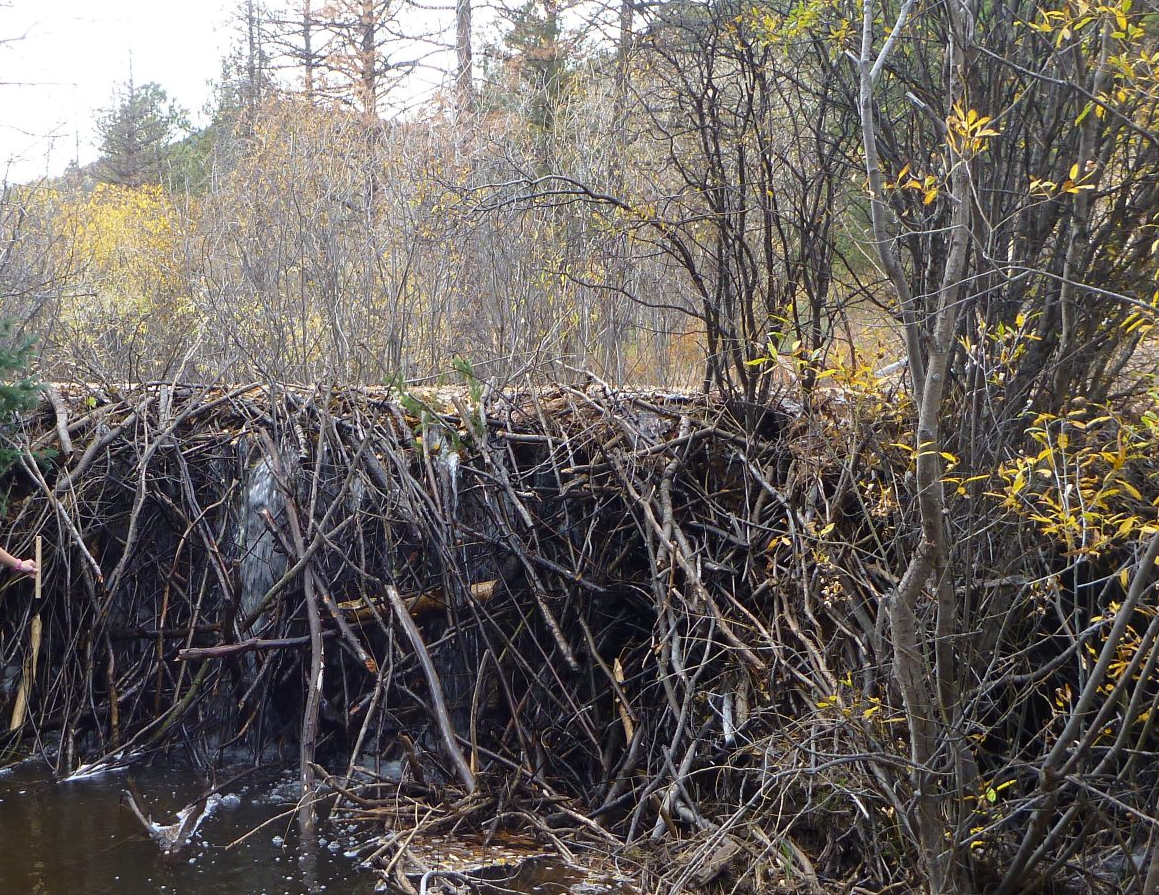
\includegraphics[scale=0.25]{./lecture_includes/beaverdam}
    \end{column}
  \end{columns}
\end{frame}





\begin{frame}{Difference-in-differences credibility crisis}

\begin{itemize}
\item I'll start with circa 2016 onward -- several grad students and assistant professors found critical pathologies with TWFE and developed solutions  
\item Many simultaneous discoveries, some redundancies, and \textbf{sudden} awareness of the issues started happening around 2017, eventually became a massive thing
\item Extreme meteoric rise, unusual for econometrics
\end{itemize}

\end{frame}

\begin{frame}{Compare with LATE paper}
  \begin{columns}
    \begin{column}{0.5\textwidth}
      \begin{itemize}
\item Compare with Imbens and Angrist 1995 LATE in \emph{Econometrica}
\item 61 annual cites the year Imbens is denied tenure at Harvard for what would later win him a Nobel Prize
      \end{itemize}
    \end{column}
    \begin{column}{0.5\textwidth}
      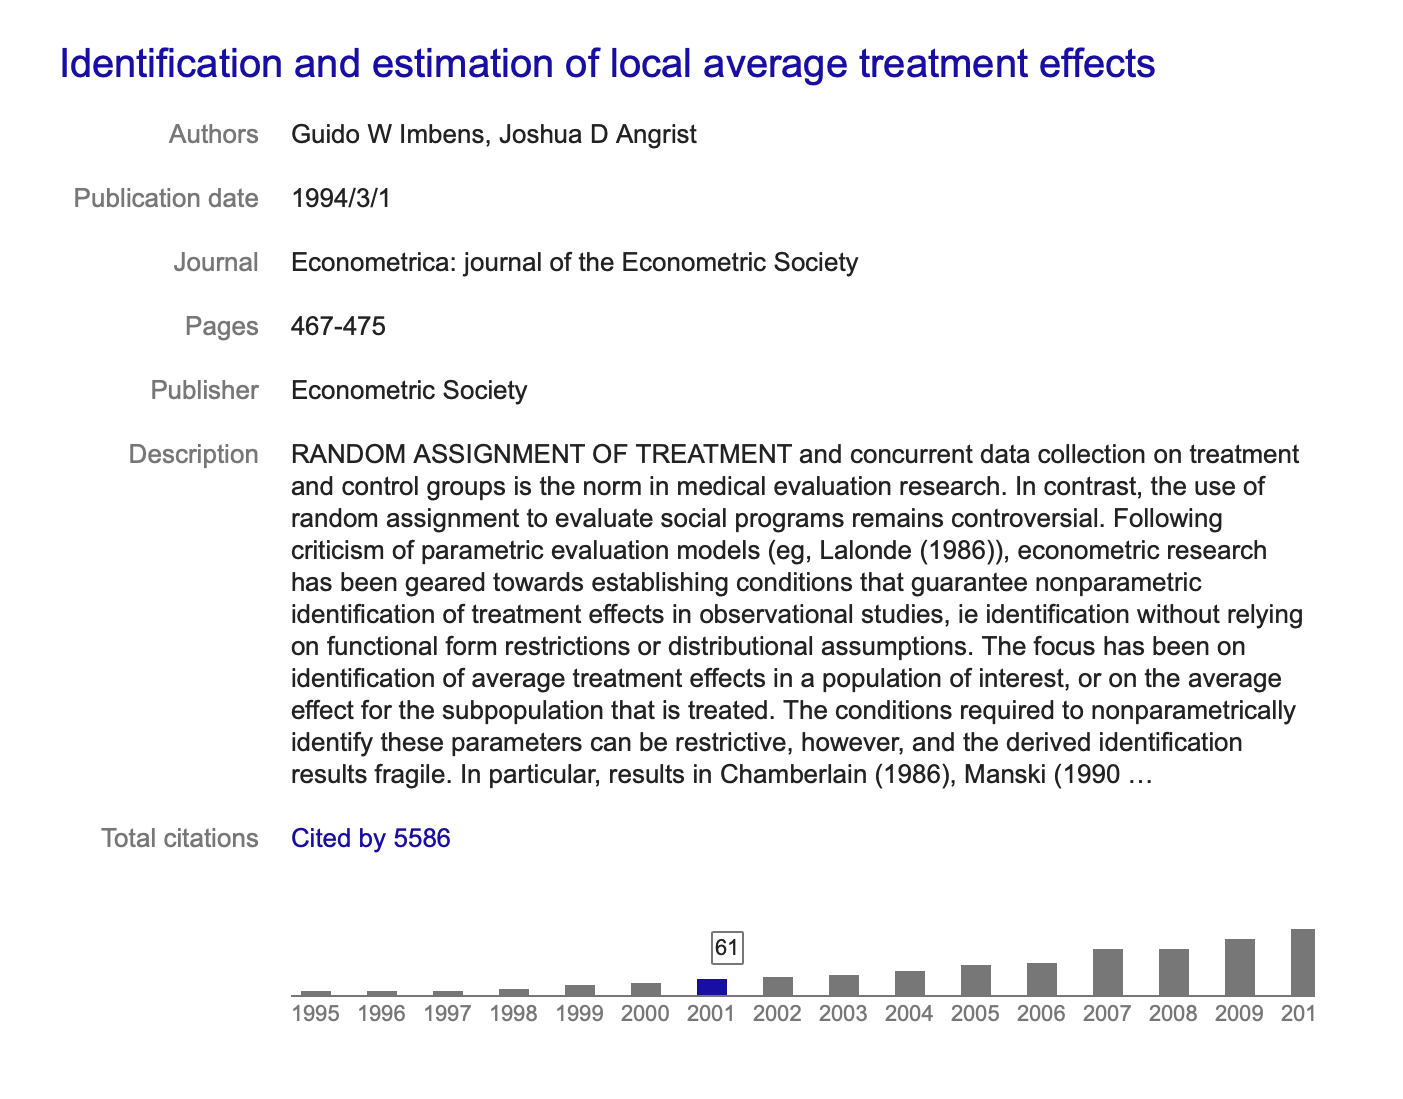
\includegraphics[scale=0.25]{./lecture_includes/guido_late}
    \end{column}
  \end{columns}
\end{frame}


\begin{frame}{Compare with synth paper}
  \begin{columns}
    \begin{column}{0.5\textwidth}
      \begin{itemize}
\item Athey and Imbens called synth the most important innovation in causal inference of the last two decades
\item Most econometrics papers, even influential ones, show slow growth
\item Something was different about diff-in-diff even before the econometricians recently shifted their attention to it
      \end{itemize}
    \end{column}
    \begin{column}{0.5\textwidth}
      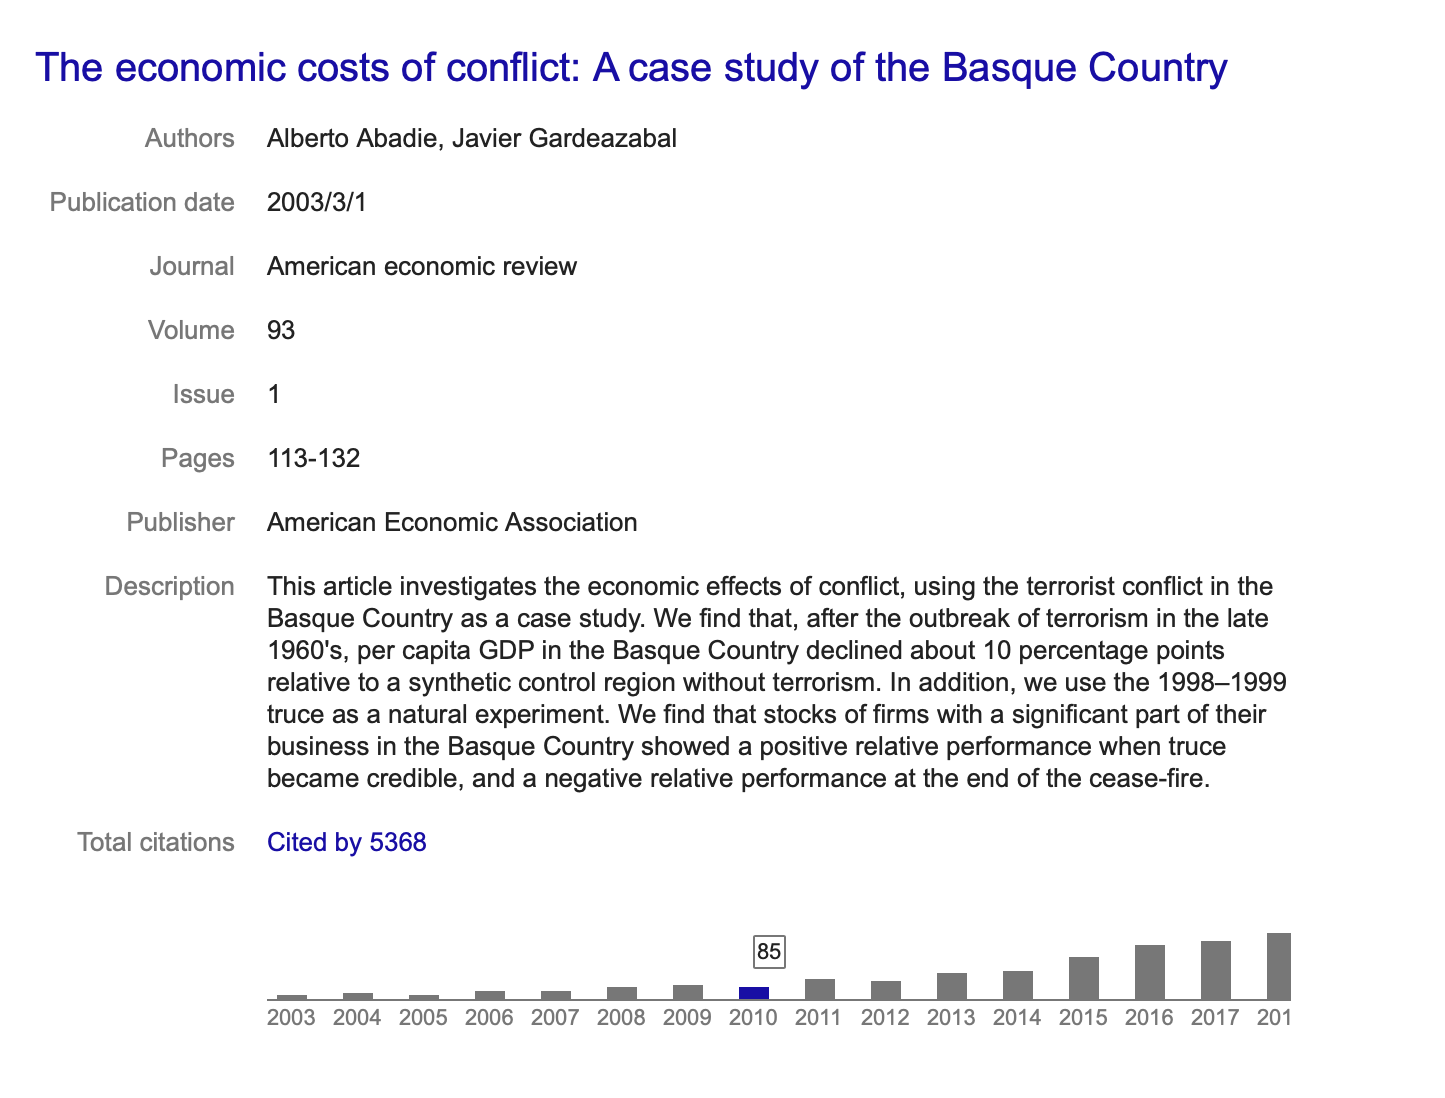
\includegraphics[scale=0.25]{./lecture_includes/basque_synth}
    \end{column}
  \end{columns}
\end{frame}


\begin{frame}{Diff-in-diff had belonged to the empiricists}

	\begin{figure}
	\caption{Currie, et al. (2020)}
	\includegraphics[scale=0.25]{./lecture_includes/currie_did.png}
	\end{figure}

\bigskip

\footnotesize

With some exception (e.g., Heckman, Ichimura and Todd 1997; Abadie 2005; Bertrand, Duflo and Mullainthan 2004), econometricians had not given it much notice

\end{frame}





\begin{frame}{Borusyak et al}
  \begin{columns}
    \begin{column}{0.5\textwidth}
      \begin{itemize}
\item Starts it all; written as grad students at Harvard
\item Goes through many revisions, posted as working paper
\item Returned to a few years ago with a third coauthor, Jahn Spiess, now R\&R at Restud
      \end{itemize}
    \end{column}
    \begin{column}{0.5\textwidth}
      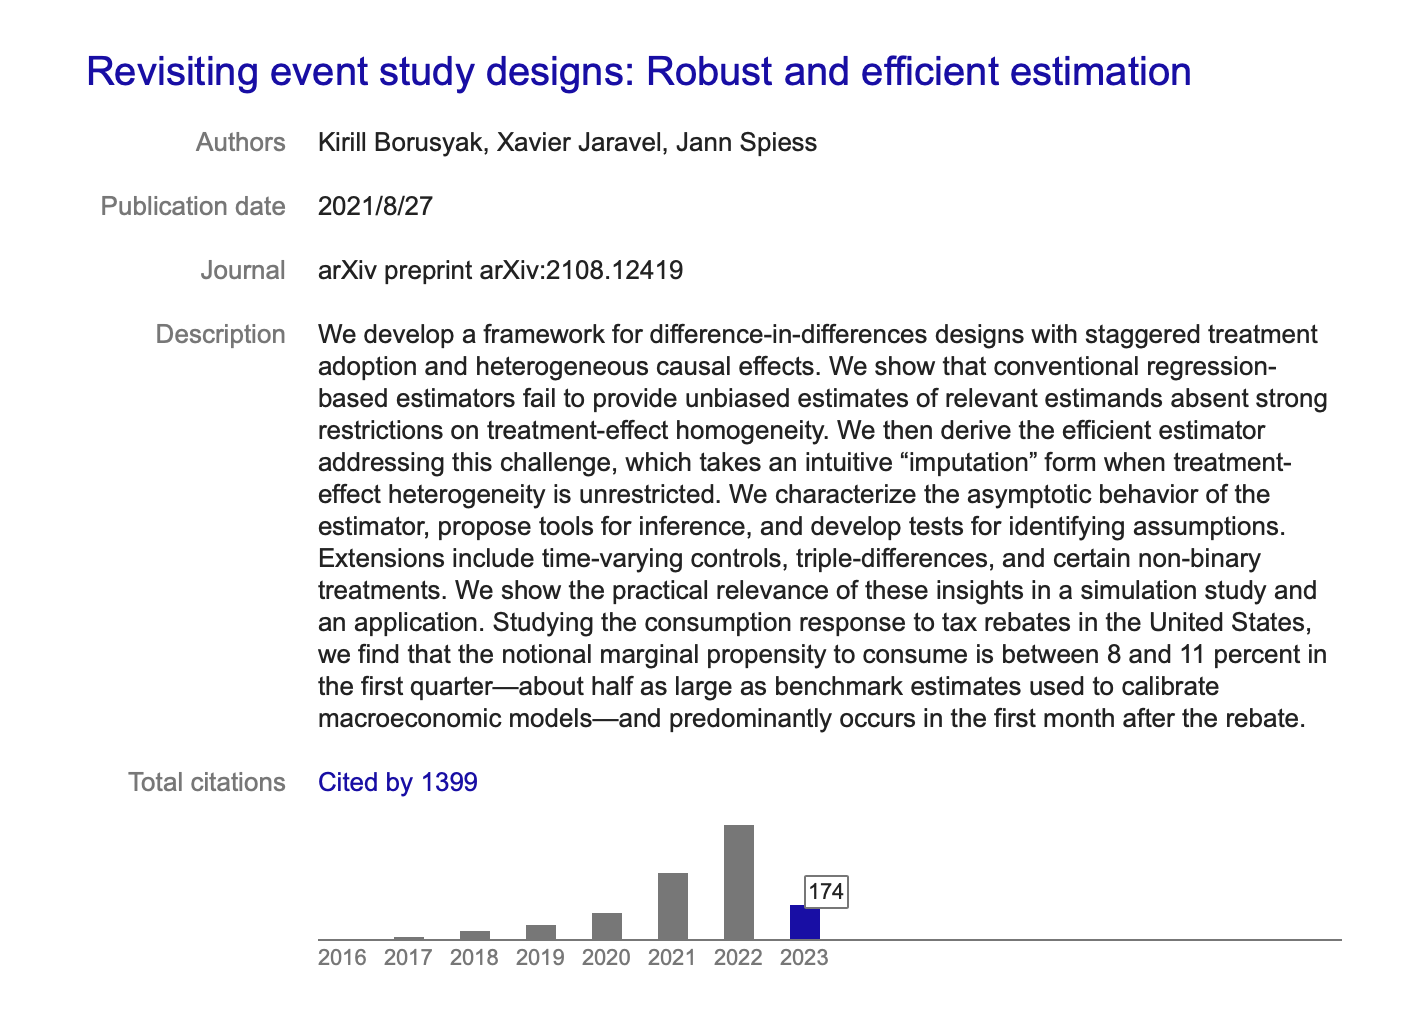
\includegraphics[scale=0.25]{./lecture_includes/kirill_cites}
    \end{column}
  \end{columns}
\end{frame}


\begin{frame}{``dCdH''}
  \begin{columns}
    \begin{column}{0.5\textwidth}
      \begin{itemize}
\item First major hit (in AER), may have been in working paper in 2017 (at least 2018)
\item Very thorough decomposition of the TWFE pathology, very general solution, included Stata code
\item Very active and talented young team (assistant profs when this was done)
      \end{itemize}
    \end{column}
    \begin{column}{0.5\textwidth}
      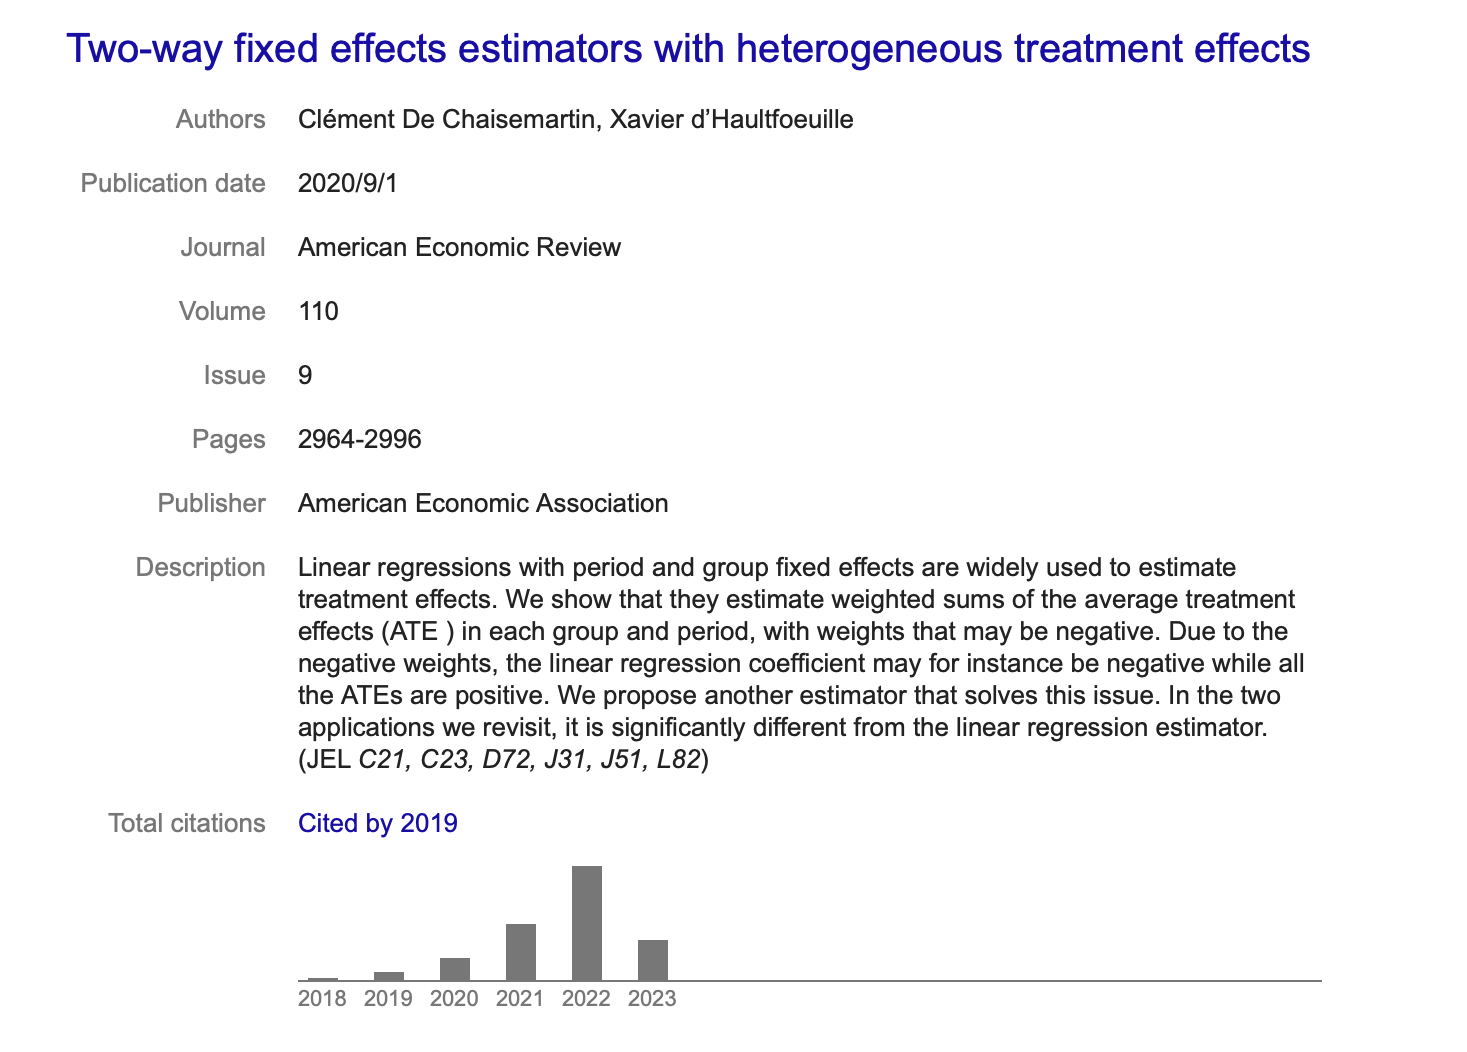
\includegraphics[scale=0.25]{./lecture_includes/dcdh_cites}
    \end{column}
  \end{columns}
\end{frame}

\begin{frame}{Goodman-Bacon}
  \begin{columns}
    \begin{column}{0.5\textwidth}
      \begin{itemize}
\item Arguably the most influential in terms of bringing attention to the problem (but no solution)
\item Begun while grad student at Michigan, published last of the crop
\item Probably Twitter network had a role as he was very active, also not an econometrician
      \end{itemize}
    \end{column}
    \begin{column}{0.5\textwidth}
      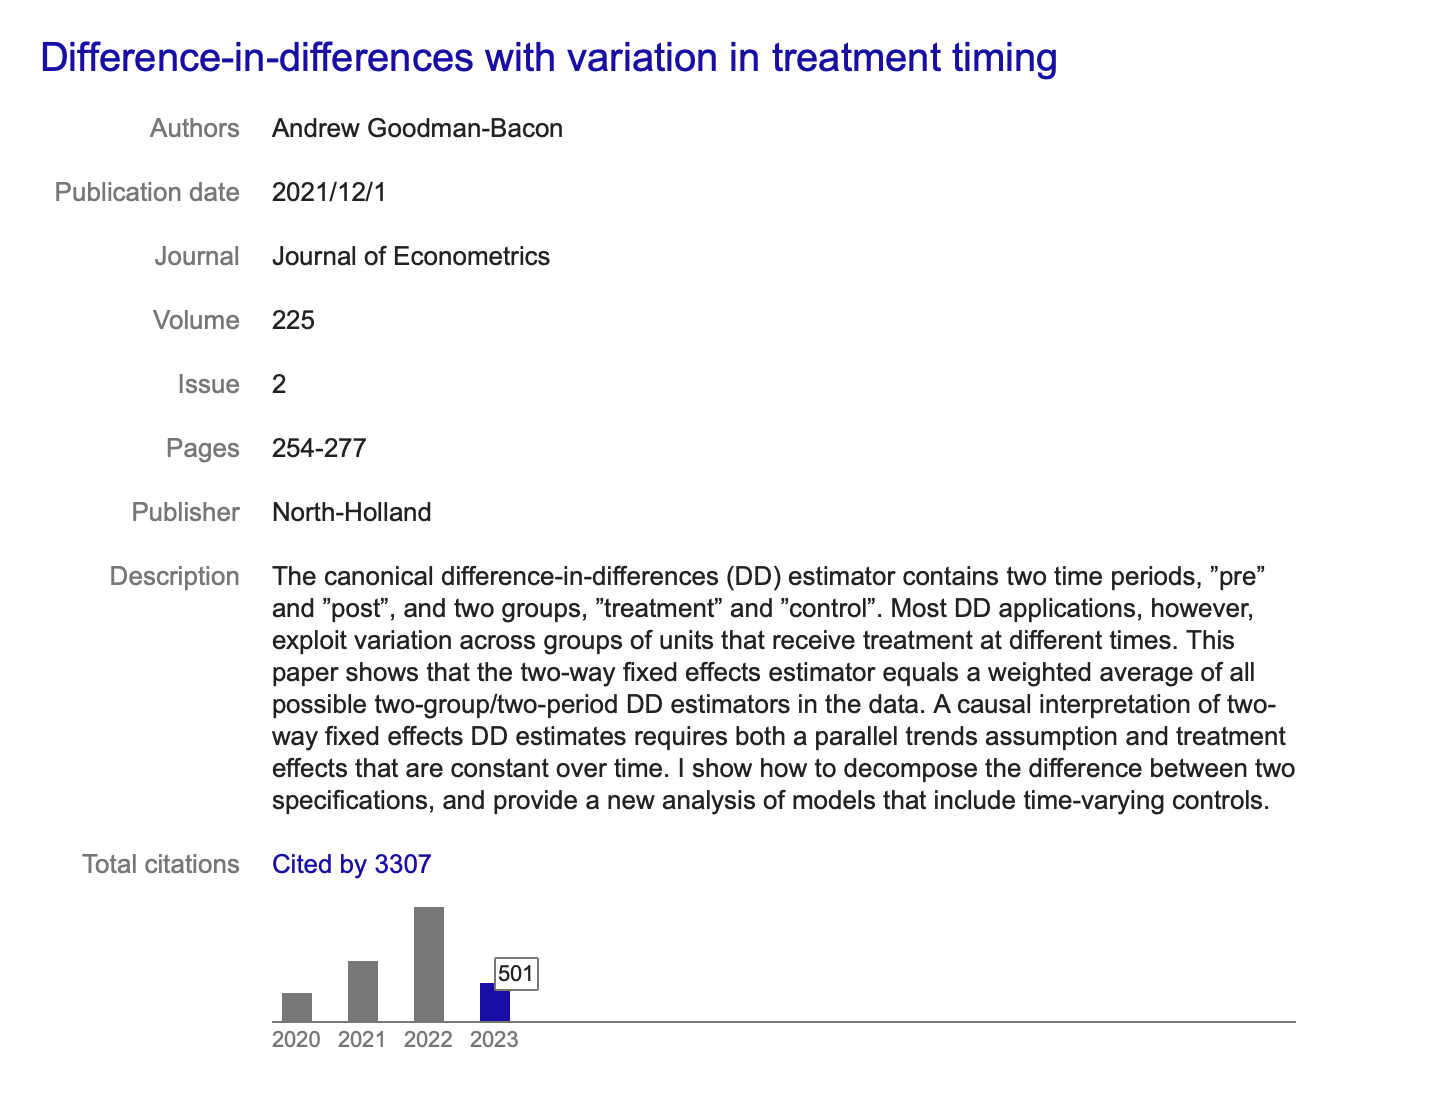
\includegraphics[scale=0.25]{./lecture_includes/andrew_cites}
    \end{column}
  \end{columns}
\end{frame}


\begin{frame}{``CS''}
  \begin{columns}
    \begin{column}{0.5\textwidth}
      \begin{itemize}
\item Second published solution to the problem, written while assistant professors at Vanderbilt and Ole Miss, 
\item Pedro is a UC3M alum (2015 grad) and Brantly is a Vanderbilt grad
\item Both are now coauthors with Andrew Goodman-Bacon
\item Introduced new terms like group-time ATT, released very tight R code (``did'')
      \end{itemize}
    \end{column}
    \begin{column}{0.5\textwidth}
      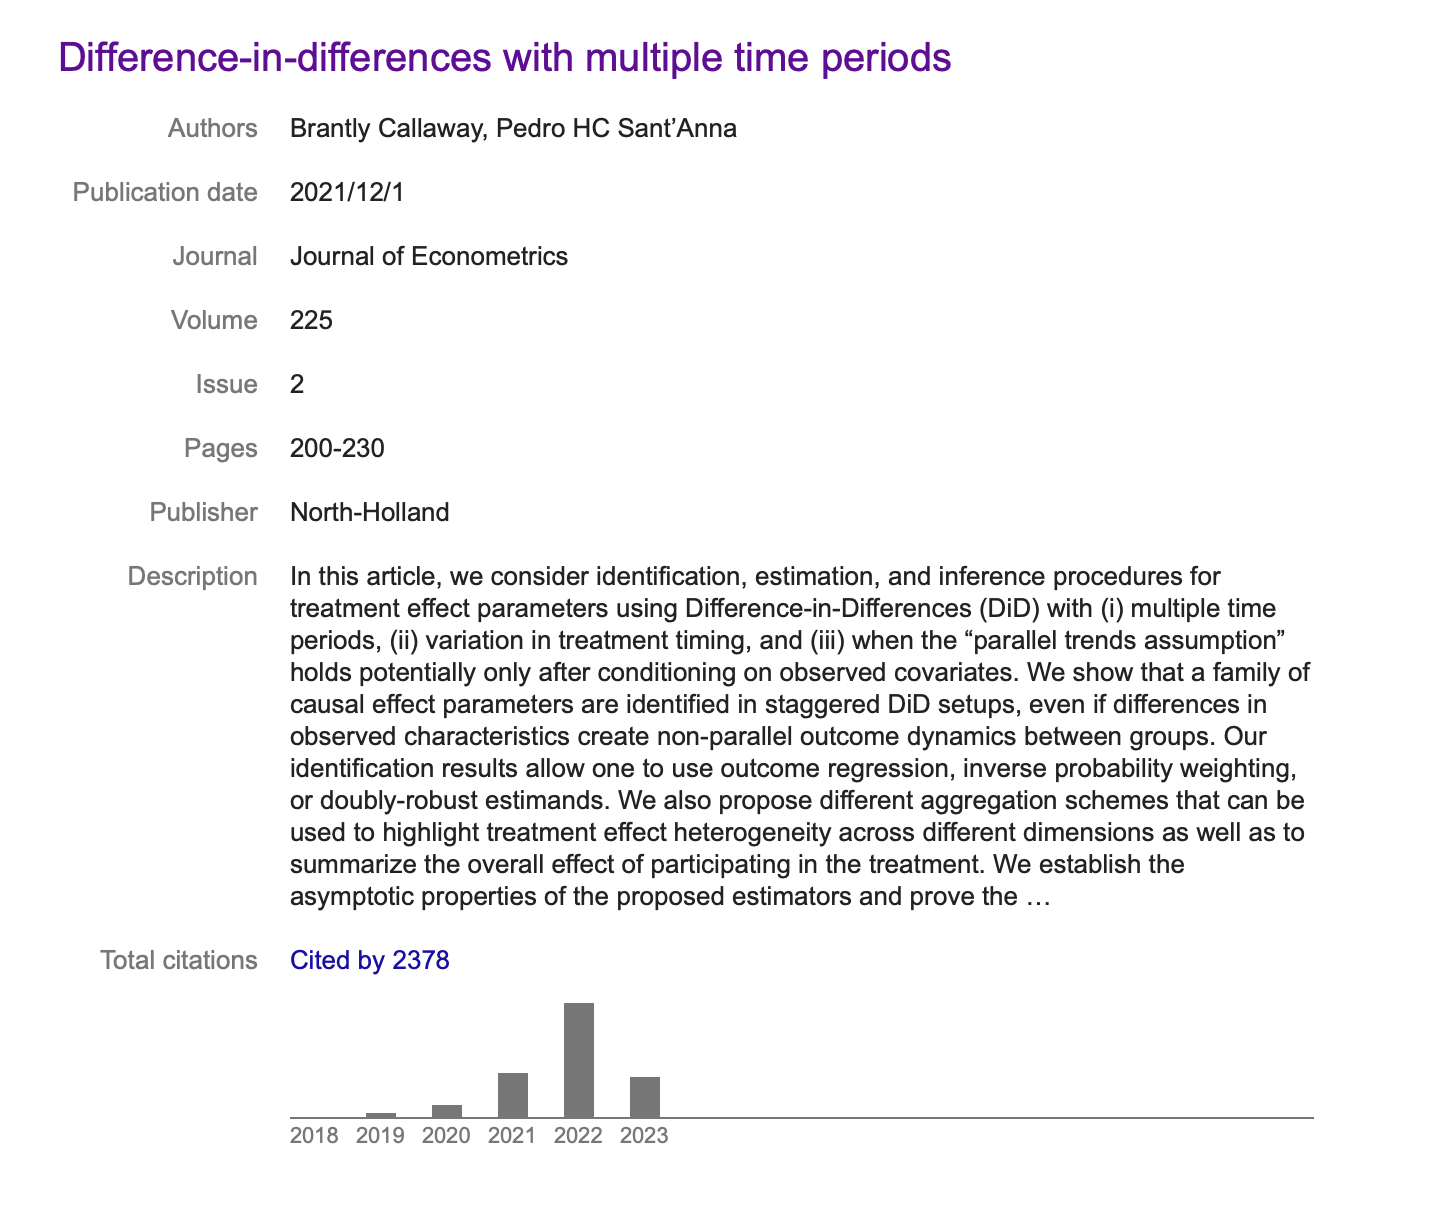
\includegraphics[scale=0.25]{./lecture_includes/pedro_cites}
    \end{column}
  \end{columns}
\end{frame}



\begin{frame}{``SA''}
  \begin{columns}
    \begin{column}{0.5\textwidth}
      \begin{itemize}
\item Third published solution to the problem, very similar to CS
\item Focus was on decomposing the event study
\item Written while grad students at MIT but Sophie Sun is now an assistant professor at CEMFI!
      \end{itemize}
    \end{column}
    \begin{column}{0.5\textwidth}
      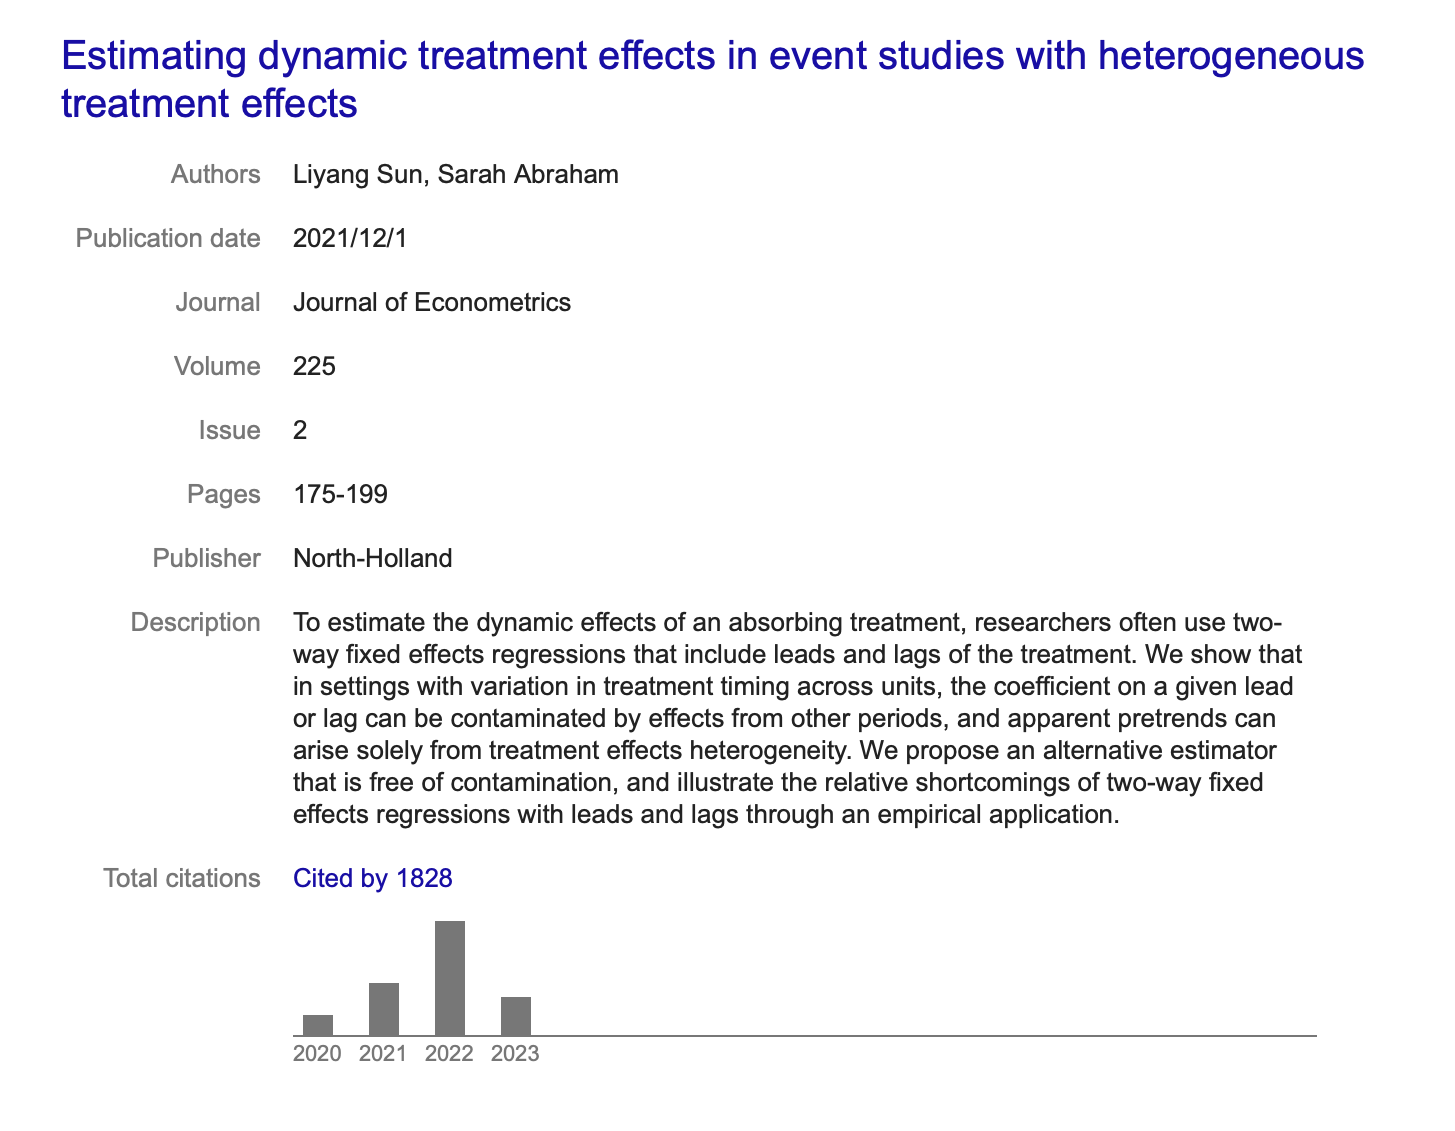
\includegraphics[scale=0.25]{./lecture_includes/sun_cites}
    \end{column}
  \end{columns}
\end{frame}

\begin{frame}{There's even more and more coming}

\begin{itemize}
\item Gardner, Wooldridge, John Roth, and on and on
\item Too many people to name at this point
\item Given the large cites, we are likely to keep seeing more on this
\item Probably shifting applied practice for the better but there are some growing pains
\end{itemize}

\end{frame}















\begin{frame}{Twoway fixed effects}

\begin{itemize}
\item When working with panel data, the so-called ``twoway fixed effects'' (TWFE) estimator was the workhorse estimator
\item And from the start, it was used with diff-in-diff
\item But at the start, it wasn't staggered adoption -- it was a much simpler design in which a group was treated in one year, and a comparison group wasn't
\end{itemize}

\end{frame}

\begin{frame}{Two OLS Models}

\begin{eqnarray}
Y_{ist} &=& \alpha_0 + \alpha_1 Treat_{is} + \alpha_2 Post_{t} + \delta (Treat_{is} \times Post_t) + \varepsilon_{ist} \\
Y_{ist} &=& \beta_0 + \delta D_{ist} + \tau_t + \sigma_s + \varepsilon_{ist}
\end{eqnarray}

\bigskip

First equation is used for simple designs when everyone is treated at once; second equation was used when different groups were treated at different times (``differential timing'')

\bigskip

First equation works; second one only sometimes works

\end{frame}






\subsection{Bacon decomposition}

\begin{frame}{Discussion of estimate}


$$Y_{ist} = \beta_0 + \delta D_{ist} + \tau_t + \sigma_s + \varepsilon_{ist}$$


\begin{itemize}
\item So that's the simple case; what about the differential timing case?  

\item If you estimate with OLS with differential timing, what does $\widehat{\delta}$ correspond to?
\item It also corresponds to the previous ``four averages and three subtractions'' -- but it's numerous of them, not just one

\end{itemize}

\end{frame}



\begin{frame}{Decomposition Preview}


\begin{itemize}
\item Andrew Goodman-Bacon decomposed $\widehat{\delta}$ and showed it is numerically identical to a weighted average of all ``four averages and three subtractions''
\item But, even before we get to causality there are unusual features
\item TWFE model assigns its own weights which are a function of the size of a ``group'' and the variance of group treatment dummies
\end{itemize}

\end{frame}



\begin{frame}{$K^2$ distinct DDs}

Let's look at 3 timing groups (a, b and c) and one untreated group (U).  With 3 timing groups, there are 9 2x2 DDs.  Here they are:


\begin{center}
\begin{tabular}{c|c|c}
\multicolumn{1}{l}{} &
\multicolumn{1}{l}{} &
\multicolumn{1}{l}{} \\
\midrule
a to b & b to a & c to a \\
a to c & b to c & c to b \\
a to U & b to U & c to U \\
\midrule
\end{tabular}
\end{center}

\bigskip

Let's return to a simpler example with only two groups -- a $k$ group treated at $t_k^*$ and an $l$ treated at $t_l^*$ plus an never-treated group called the $U$ untreated group
\end{frame} 


\begin{frame}{Terms and notation}

\begin{itemize}
\item Let there be two treatment groups (k,l) and one untreated group (U)
\item k,l define the groups based on when they receive treatment (differently in time) with k receiving it earlier than l
\item Denote $\overline{D}_k$ as the share of time each group spends in treatment status
\item Denote $\widehat{\delta}_{jb}^{2x2}$ as the canonical $2\times 2$ DD estimator for groups $j$ and b where $j$ is the treatment group and $b$ is the comparison group
\end{itemize}

\end{frame}


\imageframe{./lecture_includes/bacon_goodman_2.png}



\begin{frame}[plain]
$$\widehat{\delta}^{2x2}_{kU} = \bigg ( \overline{y}_k^{post(k)} - \overline{y}_k^{pre(k)} \bigg ) - \bigg ( \overline{y}_U^{post(k)} - \overline{y}_U^{pre(k)} \bigg ) $$
	\begin{figure}
	\includegraphics[scale=0.45]{./lecture_includes/bacon_goodman_3.png}
	\end{figure}

\end{frame}

\begin{frame}[plain]
$$\widehat{\delta}^{2x2}_{lU} = \bigg ( \overline{y}_l^{post(l)} - \overline{y}_l^{pre(l)} \bigg ) - \bigg ( \overline{y}_U^{post(l)} - \overline{y}_U^{pre(l)} \bigg ) $$
	\begin{figure}
	\includegraphics[scale=0.45]{./lecture_includes/bacon_goodman_4.png}
	\end{figure}

\end{frame}


\begin{frame}[plain]

$$\delta_{kl}^{2x2,k} = \bigg ( \overline{y}_k^{MID(k,l)} - \overline{y}_k^{Pre(k,l)} \bigg ) - \bigg ( \overline{y}_l^{MID(k,l)} - \overline{y}_l^{PRE(k,l)} \bigg ) $$

	\begin{figure}
	\includegraphics[scale=0.45]{./lecture_includes/bacon_goodman_6.png}
	\end{figure}

\end{frame}

\begin{frame}[plain]
$$\delta_{lk}^{2x2,l} = \bigg ( \overline{y}_l^{POST(k,l)} - \overline{y}_l^{MID(k,l)} \bigg ) - \bigg ( \overline{y}_k^{POST(k,l)} - \overline{y}_k^{MID(k,l)} \bigg ) $$

	\begin{figure}
	\includegraphics[scale=0.4]{./lecture_includes/bacon_goodman_7.png}
	\end{figure}

\end{frame}


	

\begin{frame}{Bacon decomposition}

$$Y_{ist} = \beta_0 + \delta D_{ist} + \tau_t + \sigma_s + \varepsilon_{ist}$$


TWFE estimate of $\widehat{\delta}$ is equal to a weighted average over all group 2x2 (of which there are 4 in this example)
\begin{eqnarray*}	
\widehat{\delta}^{TWFE} = \sum_{k \neq U} s_{kU}\widehat{\delta}_{kU}^{2x2} + \sum_{k \neq U} \sum_{l>k} s_{kl}  \bigg [ \mu_{kl}\widehat{\delta}_{kl}^{2x2,k} + (1-\mu_{kl}) \widehat{\delta}_{lk}^{2x2,l} \bigg]
\end{eqnarray*}where that first 2x2 combines the k compared to U and the l to U (combined to make the equation shorter)

\end{frame}
	


\begin{frame}{Third, the Weights}

 \begin{eqnarray*} s_{ku} &=& \frac{ n_k n_u \overline{D}_k (1- \overline{D}_k ) }{ \widehat{Var} ( \tilde{D}_{it} )} \\
s_{kl} &=& \frac{ n_k n_l (\overline{D}_k - \overline{D}_{l} ) ( 1- ( \overline{D}_k - \overline{D}_{l} )) }{\widehat{Var}(\tilde{D}_{it})} \\
\mu_{kl} &=& \frac{1 - \overline{D}_k }{1 - ( \overline{D}_k - \overline{D}_{l} )}
\end{eqnarray*}where $n$ refer to sample sizes, $\overline{D}_k (1- \overline{D}_k )$ $(\overline{D}_k - \overline{D}_{l} ) ( 1- ( \overline{D}_k - \overline{D}_{l} ))$ expressions refer to variance of treatment, and the final equation is the same for two timing groups.

\end{frame}

\begin{frame}{Weights discussion}

\begin{itemize}
\item Two things to note:
	\begin{itemize}
	\item More units in a group, the bigger its 2x2 weight is
	\item Group treatment variance weights up or down a group's 2x2
	\end{itemize}
\item Think about what causes the treatment variance to be as big as possible. Let's think about the $s_{ku}$ weights.
	\begin{itemize}
	\item $\overline{D}=0.1$. Then $0.1 \times 0.9 = 0.09$
	\item $\overline{D}=0.4$. Then $0.4 \times 0.6 =0.24$
	\item $\overline{D}=0.5$. Then $0.5 \times 0.5 = 0.25$
	\item $\overline{D}=0.6$. Then $0.6 \times 0.4 = 0.24$
	\end{itemize}
\item This means the weight on treatment variance is maximized for \emph{groups treated in middle of the panel}
\end{itemize}
\end{frame}

\begin{frame}{More weights discussion}

\begin{itemize}
\item But what about the ``treated on treated'' weights (i.e., $\overline{D}_k - \overline{D}_{l} $)  
\item Same principle as before - when the difference between treatment variance is close to 0.5, those 2x2s are given the greatest weight
\item For instance, say $t^*_k=0.15$ and $t^*_l=0.67$. Then $\overline{D}_k - \overline{D}_{l} = 0.52$.  And thus $0.52 \times 0.48 = 0.2496$.
\end{itemize}

\end{frame}


\begin{frame}{Summarizing TWFE centralities}

\begin{itemize}
\item Groups in the middle of the panel weight up their respective 2x2s via the variance weighting
\item Decomposition highlights the strange role of panel length when using TWFE
\item Different choices about panel length change both the 2x2 and the weights based on variance of treatment
\end{itemize}

\end{frame}




\begin{frame}{Back to TWFE}


$$Y_{ist} = \beta_0 + \delta D_{ist} + \tau_t + \sigma_s + \varepsilon_{ist}$$


\begin{itemize}

\item So we know that the estimate is a weighted average over all ``four averages and three subtractions'' but is that good or bad?
\item It's good if it's unbiased; it's bad if it isn't, and the decomposition doesn't tell us which unless we replace realized outcomes with potential outcomes
\item Bacon shows that TWFE estimate of $\delta$ needs two assumptions for unbiasedness:
	\begin{enumerate}
	\item variance weighted parallel trends are zero and 
	\item no dynamic treatment effects (not the case with 2x2)
	\end{enumerate}
\item Under those assumptions, TWFE estimator estimates the variance weighted ATT as a weighted average of all possible ATTs (not just weighted average of DiDs)

\end{itemize}

\end{frame}


\begin{frame}{Moving from 2x2s to causal effects and bias terms}

Let's start breaking down these estimators into their corresponding estimation objects expressed in causal effects and biases


\begin{eqnarray*}
\widehat{\delta}^{2x2}_{kU} &=& ATT_k{Post} + \Delta Y^0_k(Post(k),Pre(k)) - \Delta Y^0_U(Post(k),Pre) \\
\widehat{\delta}^{2x2}_{kl} &=& ATT_k(MID) + \Delta Y^0_k(MID,Pre) - \Delta Y^0_l(MID, Pre)
\end{eqnarray*}These look the same because you're always comparing the treated unit with an untreated unit (though in the second case it's just that they haven't been treated \emph{yet}). 

\end{frame}

\begin{frame}{The dangerous 2x2}

But what about the 2x2 that compared the late groups to the already-treated earlier groups? With a lot of substitutions we get:

\begin{eqnarray*}
\widehat{\delta}^{2x2}_{lk} &=& ATT_{l,Post(l)} + \underbrace{\Delta Y^0_l(Post(l),MID) - \Delta Y^0_k ( Post(l), MID)}_{\mathclap{\text{Parallel trends bias}}} \\
&& - \underbrace{(ATT_k(Post) - ATT_k(Mid))}_{\mathclap{\text{Heterogeneity bias!}}}
\end{eqnarray*}


\end{frame}

\begin{frame}{Substitute all this stuff into the decomposition formula}

\begin{eqnarray*}	
\widehat{\delta}^{DD} = \sum_{k \neq U} s_{kU}\widehat{\delta}_{kU}^{2x2} + \sum_{k \neq U} \sum_{l>k} s_{kl}  \bigg [ \mu_{kl}\widehat{\delta}_{kl}^{2x2,k} + (1-\mu_{kl}) \widehat{\delta}_{kl}^{2x2,l} \bigg]
\end{eqnarray*}where we will make these substitutions\begin{eqnarray*}
\widehat{\delta}_{kU}^{2x2} &=& ATT_k(Post) + \Delta Y_l^0(Post,Pre) - \Delta Y_U^0(Post, Pre) \\
\widehat{\delta}_{kl}^{2x2,k} &=& ATT_k(Mid) + \Delta Y_l^0(Mid,Pre) - \Delta Y_l^0(Mid, Pre) \\
\widehat{\delta}^{2x2,l}_{lk} &=& ATT_{l}Post(l) + \Delta Y^0_l(Post(l),MID) - \Delta Y^0_k ( Post(l), MID) \\
&&- (ATT_k(Post) - ATT_k(Mid))
\end{eqnarray*}Notice all those potential sources of biases! 

\end{frame}


\begin{frame}{Potential Outcome Notation}

\begin{eqnarray*}
p\text{ }lim\text{ } \widehat{\delta}^{TWFE}_{n\to\infty} &=& VWATT + VWPT - \Delta ATT
\end{eqnarray*}

\begin{itemize}
\item Notice the number of assumptions needed \emph{even} to estimate this very strange weighted ATT (which is a function of how you drew the panel in the first place). 
\item With dynamics, it attenuates the estimate (bias) and can even reverse sign depending on the magnitudes of what is otherwise effects in the sign in a reinforcing direction! 
\item Model can flip signs (does not satisfy a ``no sign flip property'')
\end{itemize}

\end{frame}



\subsection{Simulation}



\begin{frame}{Simulated data}

\begin{itemize}
\item 1000 firms, 40 states, 25 firms per states, 1980 to 2009 or 30 years, 30,000 observations, four groups

\item I'll impose ``unit level parallel trends'', which is much stronger than we need (we only need average parallel trends)

\item Also no anticipation of treatment effects until treatment occurs but does \emph{not} guarantee homogenous treatment effects

\item Two types of situations: constant versus dynamic treatment effects
\end{itemize}

\bigskip

\url{https://docs.google.com/spreadsheets/d/1dI67eNNE2zrX4KrkoFvej-cKxqHkM8yJdMpD-0uE4q8/edit?usp=sharing}
\end{frame}



\begin{frame}{Constant vs Dynamic Treatment Effects}
    \begin{columns}
        \column{0.5\linewidth}
        \centering
        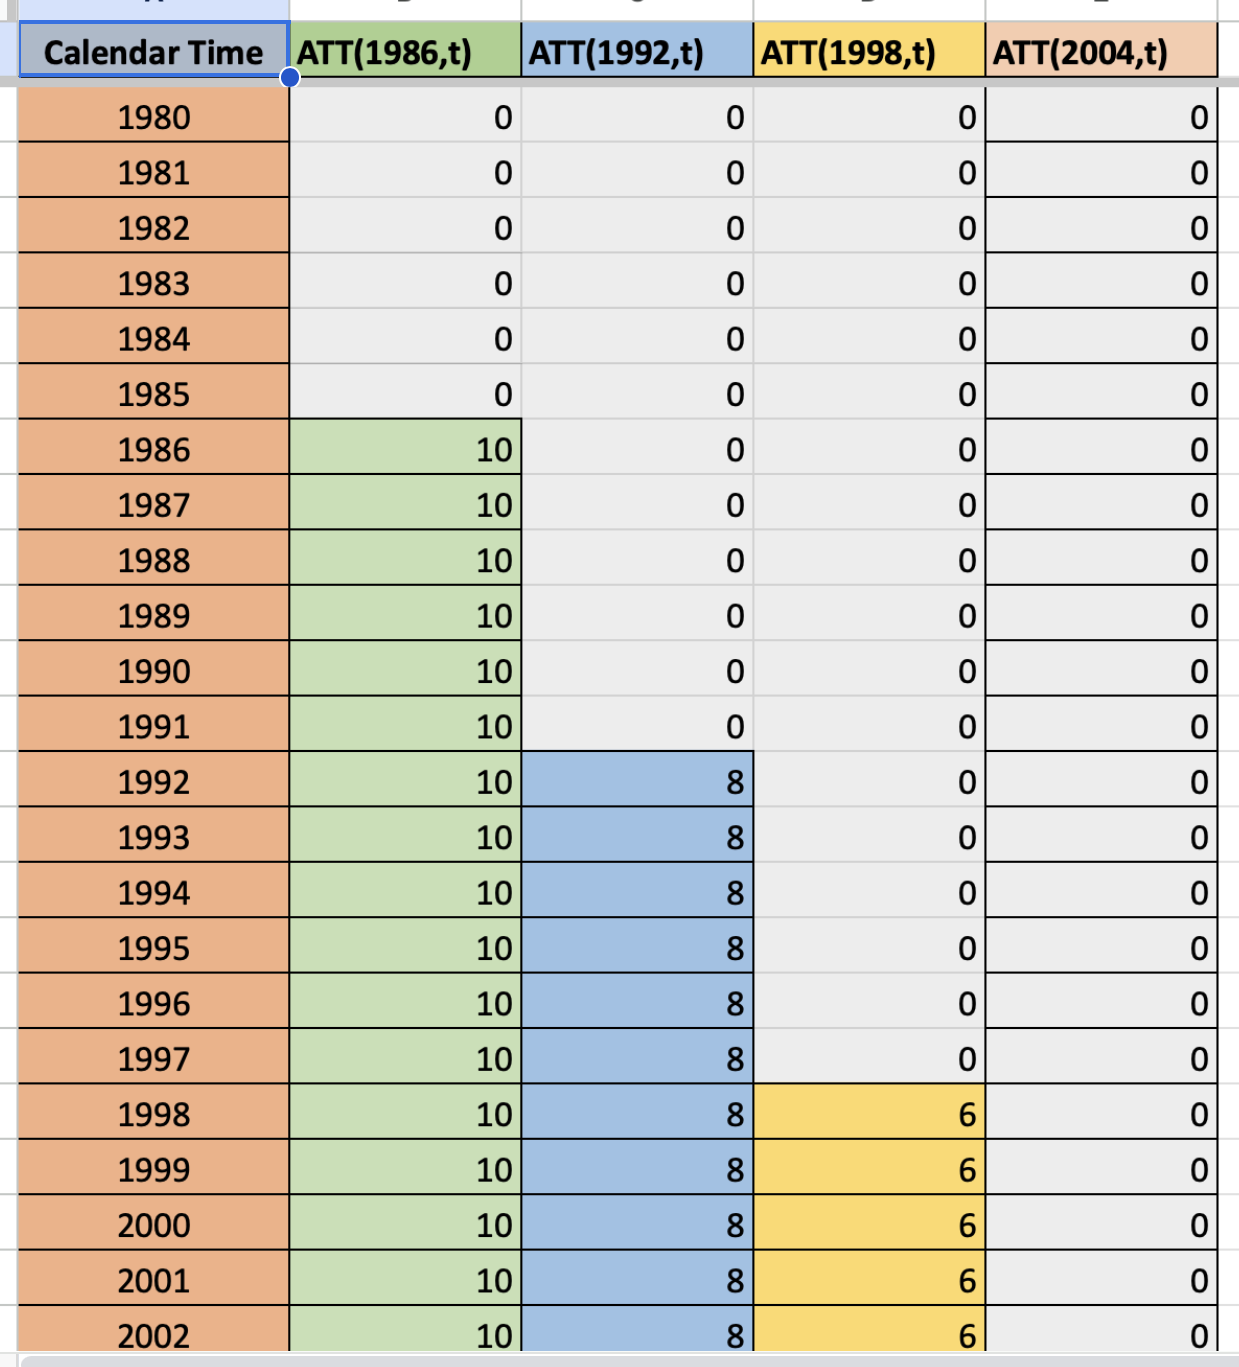
\includegraphics[height=6.5cm, width=5.5cm]{./lecture_includes/constant_te}

        \column{0.5\linewidth}
        \centering
        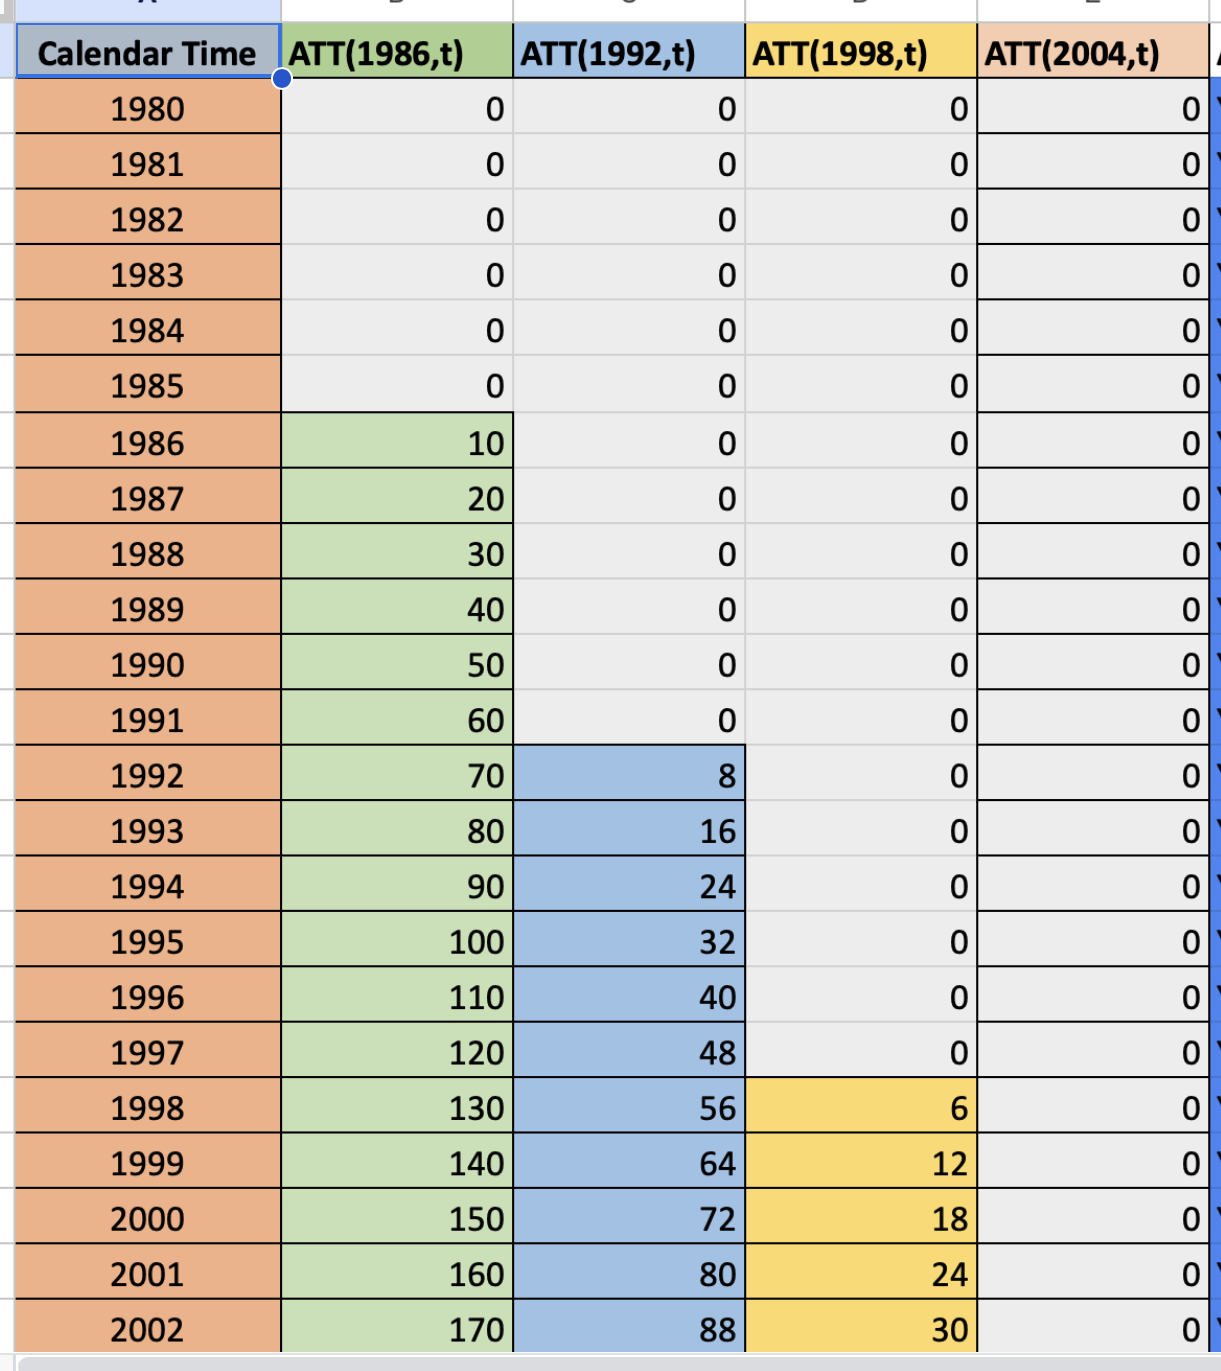
\includegraphics[height=6.5cm, width=5.5cm]{./lecture_includes/dynamic_te}
    \end{columns} 
\end{frame}




\begin{frame}{Group-time ATT}
       \begin{columns}
          \column{0.38\linewidth}
             \centering
             \includegraphics[height=6.5cm, width=5.5cm]{./lecture_includes/baker_attgt}
           \column{0.48\linewidth}
		\begin{itemize}
\item Heterogenous treatment effects across time and across groups
\item Cells are called ``group-time ATT'' (Callaway and Sant'anna 2020) or ``cohort ATT'' (Sun and Abraham 2020)
\item ATT is weighted average of all cells and $+82$ with uniform weights $1/60$
		\end{itemize}
         \end{columns} 
    \end{frame}

\begin{frame}{Estimation}

\bigskip

Estimate the following equation using OLS:

$$Y_{ist} = \alpha_i + \gamma_t +\delta D_{it} + \varepsilon_{ist}$$


\begin{table}[htbp]\centering
\small
\caption{Estimating ATT with different models}
\begin{center}
\begin{tabular}{l*{5}{c}}
\hline
\multicolumn{1}{l}{\textbf{}}&
\multicolumn{1}{c}{\textbf{Truth}}&
\multicolumn{1}{c}{\textbf{(TWFE)}}&
\multicolumn{1}{c}{\textbf{(CS)}}&
\multicolumn{1}{c}{\textbf{(SA)}}&
\multicolumn{1}{c}{\textbf{(BJS)}}\\
\hline
$\widehat{ATT}$  & 82    & -6.69*** &&&\\
\hline
\end{tabular}
\end{center}
\end{table}

The sign flipped.  Why?  Because of \emph{extreme} dynamics (i.e., $- \Delta ATT$)

\end{frame}

\begin{frame}{Bacon decomposition}
\begin{table}[htbp]\centering
\small
\caption{Bacon Decomposition (TWFE $= -6.69$)}
\begin{center}
\begin{tabular}{l*{5}{c}}
\hline
\multicolumn{1}{l}{\textbf{DD Comparison}}&
\multicolumn{1}{l}{\textbf{Weight}}&
\multicolumn{1}{l}{\textbf{Avg DD Est}}\\
\hline
Earlier T vs. Later C  &     0.500   &       51.800 \\
Later T vs. Earlier C   &    0.500    &     -65.180 \\
\midrule
T $=$ Treatment; C$ =$ Comparison \\
$(0.5*51.8) + (0.5*-65.180) = -6.69$ \\
\hline
\end{tabular}
\end{center}
\end{table}

\bigskip

While large weight on the ``late to early 2x2'' is \emph{suggestive} of an issue, these would appear even if we had constant treatment effects

\end{frame}






\section{Two solutions and a new decomposition}

\subsection{CS}



\begin{frame}{Callaway and Sant'Anna 2020}

CS is a DiD estimator used for estimating and then summarizing smaller ATT parameters under differential timing and conditional parallel trends into more policy relevant ATT parameters (either dynamic or static)


\begin{figure}
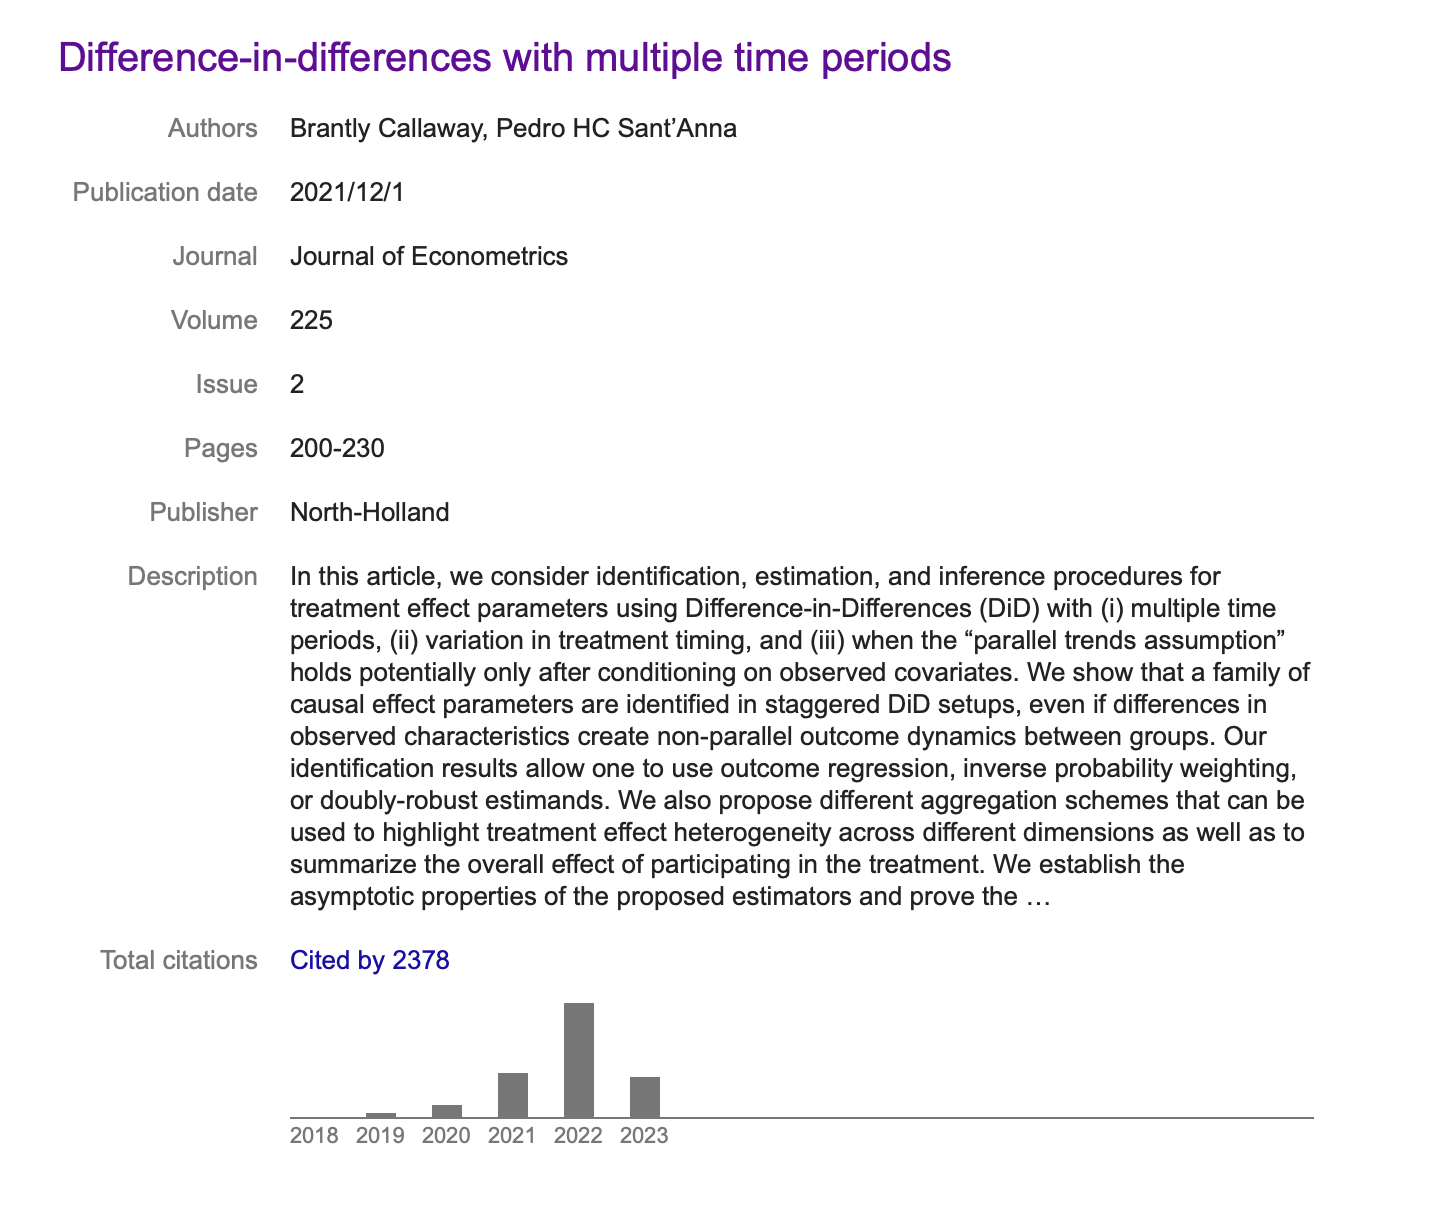
\includegraphics[scale=0.25]{./lecture_includes/pedro_cites}
\end{figure}

\end{frame}


\begin{frame}{When is CS used}

Just some examples of when you'd want to consider it:
\begin{enumerate}
\item When treatment effects differ depending on when it was adopted
\item When treatment effects change over time
\item When shortrun treatment effects are different than longrun effects
\item When treatment effect dynamics differ if people are first treated in a recession relative to expansion years
\end{enumerate}

\bigskip

CS estimates the ATT by identifying smaller causal effects and aggregating them using non-negative weights

\end{frame}






\begin{frame}{Group-time ATT}
       \begin{columns}
          \column{0.38\linewidth}
             \centering
             \includegraphics[height=6.5cm, width=5.5cm]{./lecture_includes/baker_attgt}
           \column{0.38\linewidth}
            Each cell contains that group's ATT(g,t)
\begin{eqnarray*}
ATT(g,t) = E[Y_t^1 - Y_t^0 | G_g=1]
\end{eqnarray*}CS identifies all feasible ATT(g,t)
         \end{columns} 
    \end{frame}




\begin{frame}{Group-time ATT}

Group-time ATT is the ATT for a specific group and time
\begin{itemize}
\item Groups are basically cohorts of units treated at the same time
\item Group-time ATT estimates are simple (weighted) differences in means
\item Does not directly restrict heterogeneity with respect to observed covariates, timing or the evolution of treatment effects over time
\item Allows us ways to choose our aggregations
\item Inference is the bootstrap
\end{itemize}

\end{frame}



\begin{frame}{Notation}

\begin{itemize}
\item $T$ periods going from $t=1, \dots, T$
\item Units are either treated ($D_t=1$) or untreated ($D_t=0$) but once treated cannot revert to untreated state
\item $G_g$ signifies a group and is binary.  Equals one if individual units are treated at time period $t$.
\item $C$ is also binary and indicates a control group unit equalling one if ``never treated'' (can be relaxed though to ``not yet treated'')
	\begin{itemize}
	\item Recall the problem with TWFE on using treatment units as controls
	\end{itemize}
\item Generalized propensity score enters into the estimator as a weight: $$\widehat{p(X)} = Pr(G_g=1 | X,G_g+C=1)$$
\end{itemize}

\end{frame}

\begin{frame}{Assumptions}

Assumption 1: Sampling is iid (panel data, but repeated cross-sections are possible) \\
\bigskip
Assumption 2: Conditional parallel trends (for either never treated or not yet treated) \\
\begin{eqnarray*}
E[Y_t^0 - Y_{t-1}^0 | X,G_g=1] = [Y_t^0 - Y_{t-1}^0 | X,C=1] 
\end{eqnarray*}
\bigskip
Assumption 3: Irreversible treatment \\
Assumption 4: Common support (propensity score) \\
\bigskip
Assumption 5: Limited treatment anticipation (i.e., treatment effects are zero pre-treatment)

\end{frame}

\begin{frame}{CS Estimator (the IPW version)}

\begin{eqnarray*}
ATT(g,t) = E \bigg [ \bigg ( \frac{G_g}{E[G_g]} - \frac{ \frac{\hat{p}(X)C}{1-\hat{p}(X)}}{E \bigg [ \frac{\hat{p}(X)C}{1-\hat{p}(X)} \bigg ]} \bigg ) (Y_t - Y_{g-1} ) \bigg ) \bigg ]
\end{eqnarray*}

This is the inverse probability weighting estimator.  Alternatively, there is an outcome regression approach and a doubly robust. Sant'Anna recommends DR.  CS uses the never-treated or the not-yet-treated as controls but never the already-treated 
\end{frame}




\begin{frame}{Aggregated vs single year/group ATT}

\begin{itemize}
\item The method they propose is really just identifying very narrow ATT per group time.
\item But we are often interested in  more aggregate parameters, like the ATT across all groups and all times
\item They present two alternative methods for building ``interesting parameters'' 
\item Inference from a bootstrap
\end{itemize}


\end{frame}



\begin{frame}{Group-time ATT }
             \includegraphics[scale=0.45]{./lecture_includes/baker_attgt_cs}

Question: Why didn't CS estimate all ATT(g,t)? What is ``feasible ATT''?

\end{frame}

\begin{frame}{Reporting results}
\begin{table}[htbp]\centering
\small
\caption{Estimating ATT using only pre-2004 data}
\begin{center}
\begin{tabular}{l*{5}{c}}
\hline
\multicolumn{1}{l}{\textbf{}}&
\multicolumn{1}{c}{\textbf{(Truth)}}&
\multicolumn{1}{c}{\textbf{(TWFE)}}&
\multicolumn{1}{c}{\textbf{(CS)}}&
\multicolumn{1}{c}{\textbf{(SA)}}&
\multicolumn{1}{c}{\textbf{(BJS)}}\\
\hline
$\widehat{Feasible\ ATT}$  & 68.33    & 26.81 *** & 68.34*** &&\\
\hline
\end{tabular}
\end{center}
\end{table}

TWFE is no longer negative, interestingly, once we eliminate the last group (giving us a never-treated group), but is still suffering from attenuation bias. 

\end{frame}



\subsection{SA}

\begin{frame}{Event study and differential timing}

\begin{itemize}
\item Sometimes we care about a simple summary, and sometimes we care about separating it out in time and sometimes in even more interesting ways
\item Event studies with one treatment group and one untreated group were relatively straightforward
\item Interact treatment group with calendar date to get a series of leads and lags
\item But when there are more than one treatment group, specification challenges emerge
\end{itemize}

\end{frame}



\begin{frame}{Differential timing complicates plotting sample averages}

	\begin{figure}
	\includegraphics[scale=0.25]{./lecture_includes/mml_eventstudy.png}
	\caption{Anderson, et al. (2013) display of raw traffic fatality rates for re-centered treatment states and control states with randomized treatment dates}
	\end{figure}

\end{frame}

\begin{frame}{Replicated from a project of mine}

	\begin{figure}
	\includegraphics[scale=0.5]{./lecture_includes/dd.pdf}
	\caption{Roll out of Craigslist ``personal ads'' for casual intimate encounters and birth rates using the ``randomized treatment assignment'' approach for visualization}
	\end{figure}

\end{frame}

\begin{frame}{Event study specification with TWFE}


\begin{eqnarray*}
Y_{i,t} = \alpha_i + \delta_t + \sum_{g \in G} \mu_g1\{t-E_i \in g \} + \varepsilon_{i,t}
\end{eqnarray*}

\bigskip

Coefficient $\mu_g$ on a dummy measuring the number of years prior to or after that unit was treated.  

\end{frame}

\begin{frame}[plain]
	\begin{figure}
	\includegraphics[scale=0.5]{./lecture_includes/br1544.pdf}
	\end{figure}
	
Same data as a couple slides ago, leads don't look good, so I abandoned the project. 
	
\end{frame}

\begin{frame}{Bias of TWFE Event Study Specificaiton}

\begin{itemize}
\item Bacon only focused on the static specification, and that's where the biases due to dynamics revealed itself
\item He was unable to get into the leads and lags using the FWL method he was using (``it's hard!'' - Bacon)
\item Sophie Sun and Sarah Abraham did though -- prompted by a stray comment by their professor
\item But they also unlike Bacon present a solution (which is like CS, but discovered independently)
\end{itemize}

\end{frame}



\begin{frame}{Sun and Abraham 2020}

	\begin{enumerate}
	\item SA shows a decomposition of the population regression coefficient on event study leads and lags with differential timing estimated with TWFE
	\item They show that the population regression coefficient is ``contaminated'' by information from other leads and lags (which is then later generalized by Goldsmith-Pinkham, Hull and Kolsar 2022)
	\item SA presents an alternative estimator that is a version of CS only using the ``last cohort'' as the treatment group (not the not-yet-treated)
	\item Derives the variance of the estimator instead of bootstrapping, handles covariates differently than CS, but otherwise identical
	\end{enumerate}

\end{frame}

\begin{frame}{Summarizing (cont.)}

\begin{itemize}
\item Under homogenous treatment profiles, weights sum to zero and``cancel out'' the treatment effects from other periods 
\item Under treatment effect heterogeneity, they do not cancel out and leads and lags are biased
\item They present a 3-step TWFE based alternative estimator which addresses the problems that they find
\end{itemize}

\end{frame}


\begin{frame}{Some notation and terms}

\begin{itemize}
\item As people often \textbf{bin} the data, we allow a lead or lag $l$ to appear in bin $g$ so sometimes they use $g$ instead of $l$ or $l \in g$
\item Building block is the ``cohort-specific ATT'' or $CATT_{e,l}$ -- same as ATT(g,t)
\item Our goal is to estimate $CATT_{e,l}$ with population regression coefficient $\mu_l$
\item They focus on irreversible treatment where treatment status is non-decreasing sequence of zeroes and ones
\end{itemize}

\end{frame}



\begin{frame}{Difficult notation (cont.)}

\begin{itemize}
\item The $\infty$ symbol is used to either describe the group ($E_i=\infty$) or the potential outcome ($Y^{\infty}$)
\item $Y^{\infty}_{i,t}$ is is the potential outcome for unit $i$ if it had never received treatment (versus received it later), also called the baseline outcome
\item Other counterfactuals are possible -- maybe unit $i$ isn't ``never treated'' but treated later in counterfactual
\end{itemize}
\end{frame}

\begin{frame}{More difficult notation (cont.)}

\begin{itemize}
\item Treatment effects are the difference between the observed outcome relative to the never-treated counterfactual outcome: $Y_{i,t} - Y^{\infty}_{i,t}$
\item We can take the average of treatment effects at a given relative time period across units first treated at time $E_i=e$ (same cohort) which is what we mean by $CATT_{e,l}$
\item Doesn't use $t$ index time (``calendar time''), rather uses $l$ which is time until or time after treatment date $e$ (``relative time'')
\item Think of it as ${l}=$year - treatment date
\end{itemize}

\end{frame}

\begin{frame}{Relative vs calendar event time}


\begin{figure}
\includegraphics[scale=0.2]{./lecture_includes/timetil}
\end{figure}

\end{frame}


\begin{frame}{Definition 1}

\textbf{Definition 1:} The cohort-specific ATT $l$ periods from initial treatment date $e$ is:

\begin{eqnarray*}
CATT_{e,l} = E[Y_{i,e+l} - Y^{\infty}_{i,e+l} | E_i=e]
\end{eqnarray*}

\bigskip

Fill out the second part of the Group-time ATT exercise together.

\end{frame}

\begin{frame}{TWFE assumptions}

\begin{itemize}
\item For consistent estimates of the coefficient leads and lags using TWFE model, we need three assumptions
\item For SA and CS, we only need two
\item Let's look then at the three
\end{itemize}

\end{frame}


\begin{frame}{Assumption 1: Parallel trends}

\textbf{Assumption 1: Parallel trends in baseline outcomes}: $E[Y^{\infty}_{i,t} - Y^{\infty}_{i,s} | E_i = e ]$ is the same for all $e \in supp(E_i)$ and for all $s$, $t$ and is equal to $E[Y^{\infty}_{i,t} - Y^{\infty}_{i,s} ]$

\bigskip

Lead and lag coefficients are DiD equations but once we invoke parallel trends they can become causal parameters.  This reminds us again how crucial it is to have  appropriate controls

\end{frame}


\begin{frame}{Assumption 2: No anticipation}

\textbf{Assumption 2: No anticipator behavior in pre-treatment periods}: There is a set of pre-treatment periods such that $E[Y_{i,e+l}^e - Y_{i,e+l}^{\infty} | E_i = e]=0$ for all possible leads.

\bigskip

Essentially means that pre-treatment, the causal effect is zero.  Most plausible if no one sees the treatment coming, but even if they see it coming, they may not be able to make adjustments that affect outcomes

\end{frame}


\begin{frame}{Assumption 3: Homogeneity}

\textbf{Assumption 3: Treatment effect profile homogeneity}: For each relative time period $l$, the $CATT_{e,l}$ doesn't depend on the cohort and is equal to $CATT_l$. 


\end{frame}

\begin{frame}{Treatment effect heterogeneity}

\begin{itemize}
\item Assumption 3 is violated when different cohorts experience different paths of treatment effects
\item Cohorts may differ in their covariates which affect how they respond to treatment (e.g., if treatment effects vary with age, and there is variation in age across units first treated at different times, then there will be heterogeneous treatment effects)
\item Doesn't rule out parallel trends
\end{itemize}

\end{frame}

\begin{frame}{Event study model}

Dynamic TWFE model

\begin{eqnarray*}
Y_{i,t} = \alpha_i + \delta_t + \sum_{g \in G} \mu_g1\{t-E_i \in g \} + \varepsilon_{i,t}
\end{eqnarray*}

\bigskip

We are interested in the properties of $\mu_g$ under differential timing as well as whether there are any never-treated units

\end{frame}



\begin{frame}[plain, shrink=20]
\begin{center}
\textbf{Interpreting $\widehat{\mu_g}$ under no to all assumptions}
\end{center}

\textbf{Proposition 1 (no assumptions):} The population regression coefficient on relative period bin $g$ is a linear combination of differences in trends from its own relative period $l \in g$, from relative periods $l \in g'$ of other bins $g' \neq g$, and from relative periods excluded from the specification (e.g., trimming). 

\begin{eqnarray*}
\mu_g &=& \underbrace{\sum_{l \in g} \sum_{e} w^g_{e,l} \big ( E[Y_{i,e+l} - Y^{\infty}_{i,0} | E_i = e] - E[Y^{\infty}_{i,e+l} - Y^{\infty}_{i,0}] \big )}_{\mathclap{\text{Targets}}} \\
&+& \underbrace{\sum_{g' \neq g} \sum_{l \in g'} \sum_e w^g_{e,l} \big ( E[Y_{i,e+l} - Y^{\infty}_{i,0} | E_i=e] - E[Y^{\infty}_{i,e+l} - Y^{\infty}_{i,0}] \big )}_{\mathclap{\text{Contamination from other leads and lags}}} \\
&+&  \underbrace{\sum_{l \in g^{excl}} \sum_{e} w^g_{e,l} \big ( E[Y_{i,e+l} - Y^{\infty}_{i,0} | E_i=e] - E[Y^{\infty}_{i,e+l} - Y^{\infty}_{i,0}] \big )}_{\mathclap{\text{Contamination from dropped periods}}} 
\end{eqnarray*}

\bigskip


\end{frame}

\begin{frame}{Weight ($w^g_{e,l}$) summation cheat sheet}

\begin{enumerate}
\item For relative periods of $\mu_g$ own $l \in g$, $\sum_{l \in g}\sum_ew^g_{e,l}=1$
\item For relative periods belonging to some other bin $l\in g'$ and $g' \neq g$, t $\sum_{l \in g'}\sum_ew^g_{e,l} = 0$
\item For relative periods not included in $G$, $\sum_{l \in g^{excl}} \sum_e w^g_{e,l} = -1$
\end{enumerate}

\end{frame}




\begin{frame}{Estimating the weights}

Regress $D^l_{i,t} \times 1\{E_i=e \}$ on:

\begin{enumerate}
\item all bin indicators included in the main TWFE regression, 
\item $\{ 1\{ t-E_i \in g \} \}_{g \in G}$(i.e., leads and lags) and 
\item the unit and time fixed effects
\end{enumerate}

\end{frame}


\begin{frame}{Still biased under parallel trends}

\textbf{Proposition 2}: Under the parallel trends only, the population regression coefficient on the indicator for relative period bing $g$ is a linear combination of $CATT_{e,l \in g}$ as well as $CATT_{d,l'}$ from other relative periods $l' \notin g$ with the same weights stated in Proposition 1:

\begin{eqnarray*}
\mu_g &=& \underbrace{\sum_{l \in g} \sum_e w^g_{e,l} CATT_{e,l}}_{\mathclap{\text{Desirable}}} \\
&& + \underbrace{\sum_{g' \neq g, g' \in G} \sum_{l' \in g'} \sum_e w^g_{e,l'}  CATT_{e,l'}}_{\mathclap{\text{Bias from other specified bins}}} \\
&&+ \underbrace{\sum_{l' \in g^{excl}} \sum_e w^g_{e,l'} CATT_{e,l'}}_{\mathclap{\text{Bias from dropped relative time indicators}}}
\end{eqnarray*}



\end{frame}


\begin{frame}{Still biased under parallel trends and no anticipation}

\textbf{Proposition 3}: If parallel trends holds and no anticipation holds for all $l<0$ (i.e., no anticipatory behavior pre-treatment), then the population regression coefficient $\mu_g$ for $g$ is a linear combination of post-treatment $CATT_{e,l'}$ for all $l' \geq 0$.

\begin{eqnarray*}
\mu_g &=& \sum_{l' \in g, l' \geq 0} \sum_e w^g_{e,l'} CATT_{e,l'} \\
&&+ \sum_{g' \neq g,g' \in G} \sum_{l' \in g', l' \geq 0} \sum_e w^g_{e,l'} CATT_{e,l'} \\
&&+ \sum_{l' \in g^{excl},l' \geq 0} \sum_e w^g_{w,l'} CATT_{e,l'}
\end{eqnarray*}

\end{frame}

\begin{frame}{Proposition 3 comment}

Notice how once we impose zero pre-treatment treatment effects, those terms are gone (i.e., no $l \in g, l<0$).  But the second term remains unless we impose treatment effect homogeneity (homogeneity causes terms due to weights summing to zero to cancel out). Thus $\mu_g$ may be non-zero for pre-treatment periods \emph{even though parallel trends hold in the pre period.}

\end{frame}

\begin{frame}{Proposition 4}

\textbf{Proposition 4}: If parallel trends and treatment effect homogeneity, then $CATT_{e,l}=ATT_l$ is constant across $e$ for a given $l$, and the population regression coefficient $\mu_g$ is equal to a linear combination of $ATT_{l \in g}$, as well as $ATT_{l' \notin g}$ from other relative periods

\begin{eqnarray*}
\mu_g &=& \sum_{l \in g} w^g_l ATT_l \\
&&+ \sum_{g' \neq g} \sum_{l' \in g'} w^g_{l'} ATT_{l'} \\
&&+ \sum_{l' \in g^{excl}} w^g_{l'}ATT_{l'}
\end{eqnarray*}


\end{frame}

\begin{frame}{Simple example}


Balanced panel $T=2$ with cohorts $E_i \in \{1,2 \}$. For illustrative purposes, we will include bins $\{-2,0\}$ in our calculations but drop $\{-1,1\}$. 


\end{frame}

\begin{frame}{Simple example}

\begin{eqnarray*}
\mu_{-2} &=& \underbrace{CATT_{2,-2}}_{\mathclap{\text{own period}}} + \underbrace{\frac{1}{2}CATT_{1,0} - \frac{1}{2} CATT_{2,0}}_{\mathclap{\text{other included bins}}} \\
&&+ \underbrace{ \frac{1}{2} CATT_{1,1} - CATT_{1,-1} - \frac{1}{2} CATT_{2,-1} }_{\mathclap{\text{Excluded bins}}}
\end{eqnarray*}

\begin{itemize}
\item Parallel trends gets us to all of the $CATT$
\item No anticipation makes $CATT=0$ for all $l<0$ (all $l<0$ cancel out)
\item Homogeneity cancels second and third terms
\item Still leaves $\frac{1}{2} CATT_{1,1}$ -- you chose  to exclude a group with a treatment effect
\end{itemize}Lesson: drop the relative time indicators on the left, not things on the right, bc lagged effects will contaminate through the excluded bins


\end{frame}


\begin{frame}{Robust event study estimation}


\begin{itemize}
\item All the robust estimators under differential timing have solutions and they all skip over forbidden contrasts. 
\item Sun and Abraham (2020) propose a 3-step interacted weighted estimator (IW) using last treated group as control group
\item Callaway and Sant'anna (2020) estimate group-time ATT which can be a weighted average over relative time periods too but uses ``not-yet-treated'' as control
\end{itemize}

\end{frame}




\begin{frame}{Interaction-weighted estimator}

\begin{itemize}
\item \textbf{Step one}: Do this DD regression and hold on to $\widehat{\delta}_{e,l}$
\end{itemize}

\begin{eqnarray*}
Y_{i,t} = \alpha_i + \lambda_t + \sum_{e \notin C} \sum_{l \neq -1} \delta_{e,l} \big (1 \{ E_i = e \} \cdot D_{i,t}^l \big ) + \varepsilon_{i,t}
\end{eqnarray*}


\bigskip

Can use never-treated or last-treated cohort. Drop always treated. The $\delta_{e,l}$ is a DD estimator for $CATT_{e,l}$ with particular choices for pre-period and cohort controls

\end{frame}


\begin{frame}{Interaction-weighted estimator}

\begin{itemize}
\item \textbf{Step two}: Estimate weights using sample shares of each cohort in the relevant periods:
\end{itemize}

\begin{eqnarray*}
Pr(E_i=e|E_i \in [-l,T-l])
\end{eqnarray*}

\end{frame}

\begin{frame}{Interaction-weighted estimator}

\begin{itemize}
\item \textbf{Step three}: Take a weighted average of estimates for $CATT_{e,l}$ from Step 1 with weight estimates from step 2
\end{itemize}


\begin{eqnarray*}
\widehat{v}_g = \frac{1}{|g|} \sum_{l \in g} \sum_e \widehat{\delta}_{e,l} \widehat{Pr} \{ E_i=e | E_i \in [-l,T-l]\}
\end{eqnarray*}


\end{frame}

\begin{frame}{Consistency and Inference}


\begin{itemize}
\item Under parallel trends and no anticipation, $\widehat{\delta}_{e,l}$ is consistent, and sample shares are also consistent estimators for population shares. 
\item Thus IW estimator is consistent for a weighted average of $CATT_{e,l}$ with weights equal to the share of each cohort in the relevant period(s).
\item They show that each IW estimator is asymptotically normal and derive its asymptotic variance. Doesn't rely on bootstrap like CS.
\end{itemize}

\end{frame}

\begin{frame}{DD Estimator of CATT}

\textbf{Definition 2}: DD estimator with pre-period $s$ and control cohorts $C$ estimates $CATT_{e,l}$ as:

\begin{eqnarray*}
\widehat{\delta_{e,l}} = \frac{ E_N \big [ \big ( Y_{i, e+l} - Y_{i,s} \big ) \times 1\{E_i=e\} \big ]}{E_N[1 \{E_i=e\} ]} - \frac{E_N \big [ \big ( Y_{i,e+l} \times 1 \{E_i \in C \} ]}{E_N [1 \{ E_i \in C \}]}
\end{eqnarray*}


\textbf{Proposition 5}: If parallel trends and no anticipation both hold for all pre-periods, then the DD estimator using any pre-period and non-empty control cohorts (never-treated or not-yet-treated) is an unbiased estimate for $CATT_{e,l}$

\end{frame}

\begin{frame}{Software}

\begin{itemize}
\item \textbf{Stata}: eventstudyinteract (can be installed from ssc)
\item \textbf{R}: fixest with subab() option (see \url{https://lrberge.github.io/fixest/reference/sunab.html/})
\end{itemize}


\end{frame}


\begin{frame}{Reporting results}
\begin{table}[htbp]\centering
\small
\caption{Estimating ATT}
\begin{center}
\begin{tabular}{l*{5}{c}}
\hline
\multicolumn{1}{l}{\textbf{}}&
\multicolumn{1}{c}{\textbf{(Truth)}}&
\multicolumn{1}{c}{\textbf{(TWFE)}}&
\multicolumn{1}{c}{\textbf{(CS)}}&
\multicolumn{1}{c}{\textbf{(SA)}}&
\multicolumn{1}{c}{\textbf{(BJS)}}\\
\hline
$\widehat{Feasible\ ATT}$  & 68.33    & 26.81*** & 68.34*** & 68.33***&\\
\hline
\end{tabular}
\end{center}
\end{table}

\end{frame}

\begin{frame}{Computing relative event time leads and lags }
             \includegraphics[scale=0.45]{./lecture_includes/sa_leads}

Two things to notice: (1) there only 17 lags with robust models but will be 24 with TWFE; (2) changing colors mean what?

\end{frame}

\begin{frame}{Comparing TWFE and SA }

\begin{figure}
\begin{center}
             \includegraphics[scale=0.4]{./lecture_includes/twfe_sa_event}
\end{center}
\end{figure}

Question: why is TWFE \emph{falling} pre-treatment?  Why is SA rising, but jagged, post-treatment?

\end{frame}

\subsection{Some opinions and an application}

\begin{frame}{Advice}

\begin{itemize}
\item DiD will remain popular for a while, and if anything all this new DiD has brought even more attention to it
\item But now things are changing -- how do we write the papers?  Not just how do we estimate parameters
\item Papers are a combination of science and rhetoric -- let's look at a new one
\item Braghieri, Levy and Makarin (2022), ``Social Media and Mental Health'', \emph{American Economic Review}, 112(11): 3660-3693
\end{itemize}

\end{frame}


\begin{frame}{Big picture}

\begin{itemize}
\item Widely cited that social media causes mental health problems in youth
\item Anecdotal, documentaries, but no causal evidence (``slim to none'')
\item Study will use staggered rollout of Facebook platform to college campuses from 2004 to 2006 to estimate the effect on aggregate mental health scores from a survey
\item You be the judge, but they present what in most cases would be strong evidence that Facebook harmed college students mental health

\end{itemize}

\end{frame}

\begin{frame}{Many things to like}

\begin{itemize}
\item Important question: mental health, suicide, review descriptive stats together
\item Strong design: staggered rollout
\item Event study is eye popping
\item Mechanism and main results
\item Very interesting dataset

\end{itemize}

\end{frame}


\begin{frame}{Fives parts of a strong DiD}

\begin{enumerate}

\item \textbf{Bite}: They cannot really show much here.  No data on Facebook usage.  More an ITT
\item \textbf{Main Results}: Estimated effect on mental health measures
\item \textcolor{red}{Mechanism}: Speculative
\item \textbf{Falsifications}: I can't really see very strong falsifications either.
\item \textbf{Event studies}: POW.  Just wait

\end{enumerate}

\end{frame}

\begin{frame}{Mechanism}

\begin{tikzpicture}[
  ->,>=stealth, % defines the style of the edge/arrow
  shorten >=1pt, % shortens the arrow at the target node
  auto,
  node distance=3cm, % defines the space between the nodes
  thick,
  main node/.style={circle,fill=blue!20,draw,font=\sffamily\Large\bfseries}, % style of the main nodes
  dashed node/.style={circle,fill=blue!20,draw,dashed,font=\sffamily\Large\bfseries} % style of the dashed node
  ]

  \node[main node] (D) {D}; 
  \node[main node] (M) [above right of=D] {M}; 
  \node[main node] (X) [below right of=D] {X};
  \node[main node] (Y) [right of=M, below of=M] {Y};
  \node[dashed node] (U) [above of=M] {U};
  
  \path[every node/.style={font=\sffamily\small}]
    (D) edge node {} (M)
    (D) edge node {} (X)
    (M) edge node {} (Y)
    (X) edge node {} (Y)
    (U) edge[dashed] node {} (D)
    (U) edge[dashed] node {} (M)
    (U) edge[dashed] node {} (X)
    (U) edge[dashed] node {} (Y);
\end{tikzpicture}

\end{frame}

\begin{frame}{Mechanism}

\begin{itemize}
\item $D$ is the treatment variable, and the ATT is over all possible channels, but what if you want to think $M$ is the mechanism
\item When you can't rule out competing theories with falsifications, you have to try and build the case that the effect is coming through a channel
\item Rule out $X$ and provide evidence for $M$
\item Goal here is to try and present evidence (not proof) that it's probably the story you're saying

\end{itemize}

\end{frame}



\begin{frame}{Ruling out alternative mechanism}

\begin{tikzpicture}[
  ->,>=stealth, % defines the style of the edge/arrow
  shorten >=1pt, % shortens the arrow at the target node
  auto,
  node distance=3cm, % defines the space between the nodes
  thick,
  main node/.style={circle,fill=blue!20,draw,font=\sffamily\Large\bfseries}, % style of the main nodes
  dashed node/.style={circle,fill=blue!20,draw,dashed,font=\sffamily\Large\bfseries} % style of the dashed node
  ]

  \node[main node] (D) {D}; 
  \node[main node] (M) [right of=D] {M}; 
  \node[main node] (Y) [right of=M] {Y};
  \node[dashed node] (U) [above of=M] {U};
  
  \path[every node/.style={font=\sffamily\small}]
    (D) edge node {} (M)
    (M) edge node {} (Y)
    (U) edge[dashed] node {} (D)
    (U) edge[dashed] node {} (M)
    (U) edge[dashed] node {} (Y);
\end{tikzpicture}


\end{frame}





\begin{frame}{Mechanism}

\begin{itemize}

\item Story is interpersonal comparisons which they try to show 
\item We can discuss how plausible we found it, but ask yourself at the end -- did the event study help you believe it?  Why/why not?

\end{itemize}

\end{frame}

\begin{frame}{Data on Facebook}

\begin{itemize}

\item Ingenious use of the Wayback Time Machine
\item Looked at over 700 schools using Facebook screen shots
\item When Facebook first mentions a school on its front page, that school is marked as having gotten Facebook

\end{itemize}

\end{frame}


\begin{frame}{New schools being adopted}
\begin{center}

\includegraphics[scale=0.35]{./lecture_includes/timemachine_1}
\end{center}
\end{frame}

\begin{frame}{New schools being adopted}
\begin{center}

\includegraphics[scale=0.35]{./lecture_includes/timemachine_2}
\end{center}
\end{frame}


\begin{frame}{Data on college students}

\begin{itemize}
\item NCHA Data is survey administered to college students on a semi-annual basis by American College Health Assoc
\item Inquires about demographics, physical health, mental health, alcohol and drug use, sexual behaviors, and perception of these behaviors by peers
\item ACHA merged a treatment indicator to each respondent based on Facebook dataset provided to them so that privacy could be maintained

\end{itemize}

\end{frame}

\begin{frame}{Mental health}

\begin{itemize}

\item Self-reported symptoms are standard medical practice in mental health -- DSM-5 relies on self-reports such as difficulty sleeping, fatigue, feelings of guilt, suicidal ideation
\item No data on Facebook or social media usage so this is ITT version of the ATT
\item Respondent answers to the questions are aggregated into indices such as \emph{poor mental health} where larger numbers are worse

\end{itemize}

\end{frame}

\begin{frame}{Main TWFE Model}

\begin{equation}
Y_{icgt} = \alpha_g + \delta_t + \beta \times Facebook_{gt} + X_i \times \gamma + X_c \times \psi + \varepsilon_{icgt}
\end{equation}

\bigskip

$Y_{icgt}$ is an outcome for person $i$ in wave $t$ attending college $c$ in expansion group $g$; $\alpha_g$ is expansion-group or college fixed effects; $\delta_t$ are survey-wave fixed effects; $Facebook_{gt}$ indicates the respondents' campus has Facebook by time $t$ at expansion group $g$; $X_i$ and $X_c$ are individual and college-level controls; and standard errors are clustered at college level.

\bigskip

$\widehat{\beta}$ identifies the ATT under parallel trends in the robust models


\end{frame}

\begin{frame}{Robustness}

\begin{itemize}

\item Main static results will all be in TWFE, but appendix shows other methods like CS and SA 
\item Event studies will show all models including some we haven't reviewed
\item Growing popularity to show ``all the robust DiD'' models so that readers can see you aren't cherry picking

\end{itemize}

\end{frame}



\begin{frame}
\begin{center}
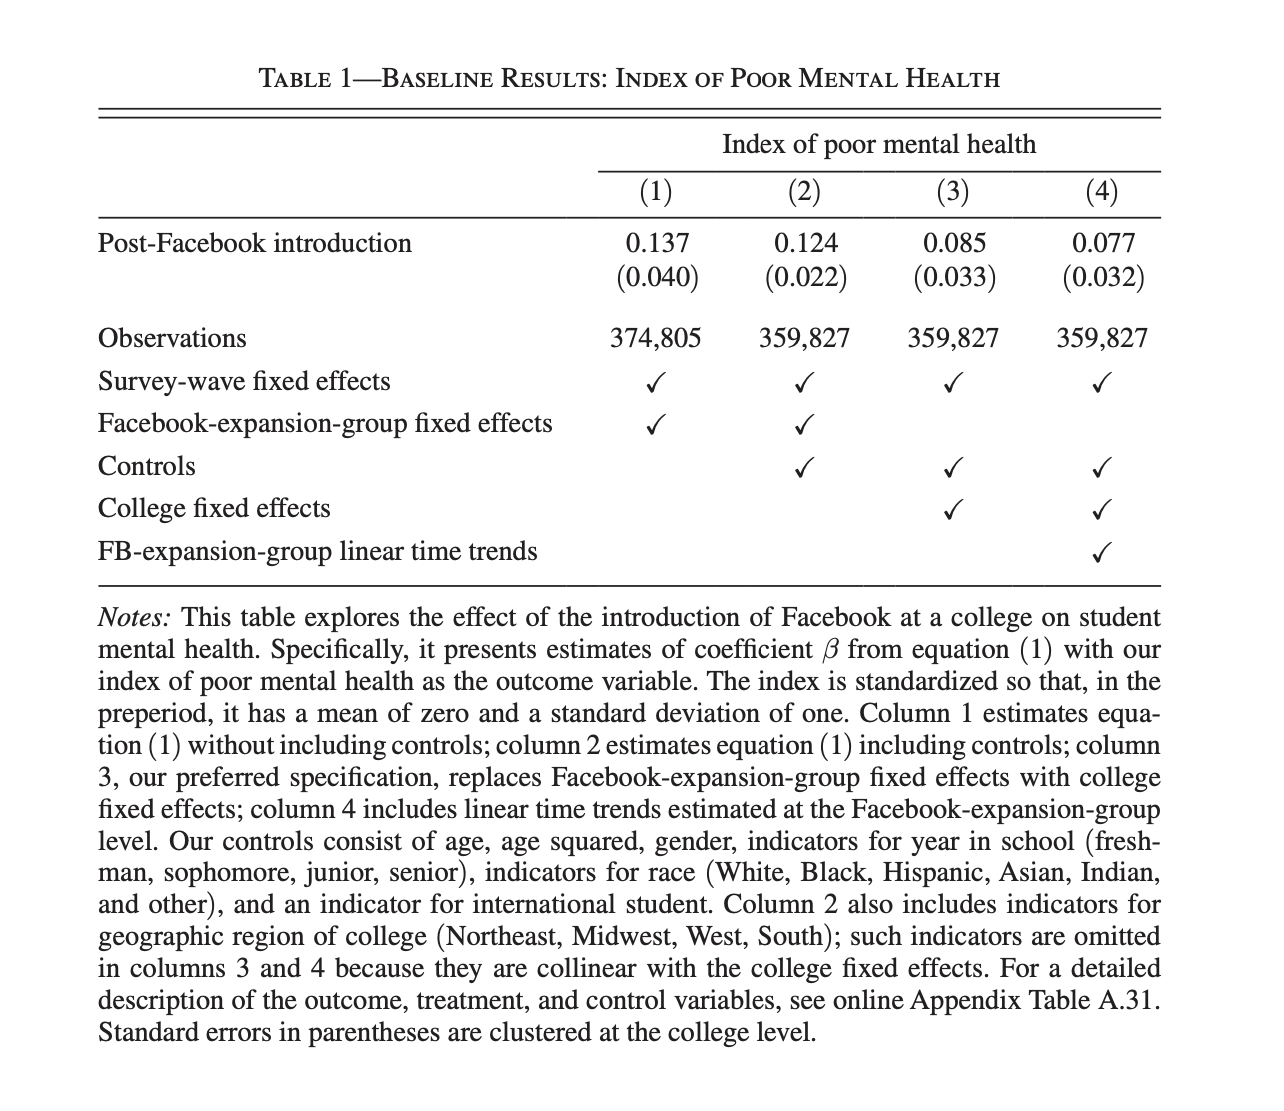
\includegraphics[scale=0.35]{./lecture_includes/facebook_1}
\end{center}
\end{frame}

\begin{frame}
\begin{center}
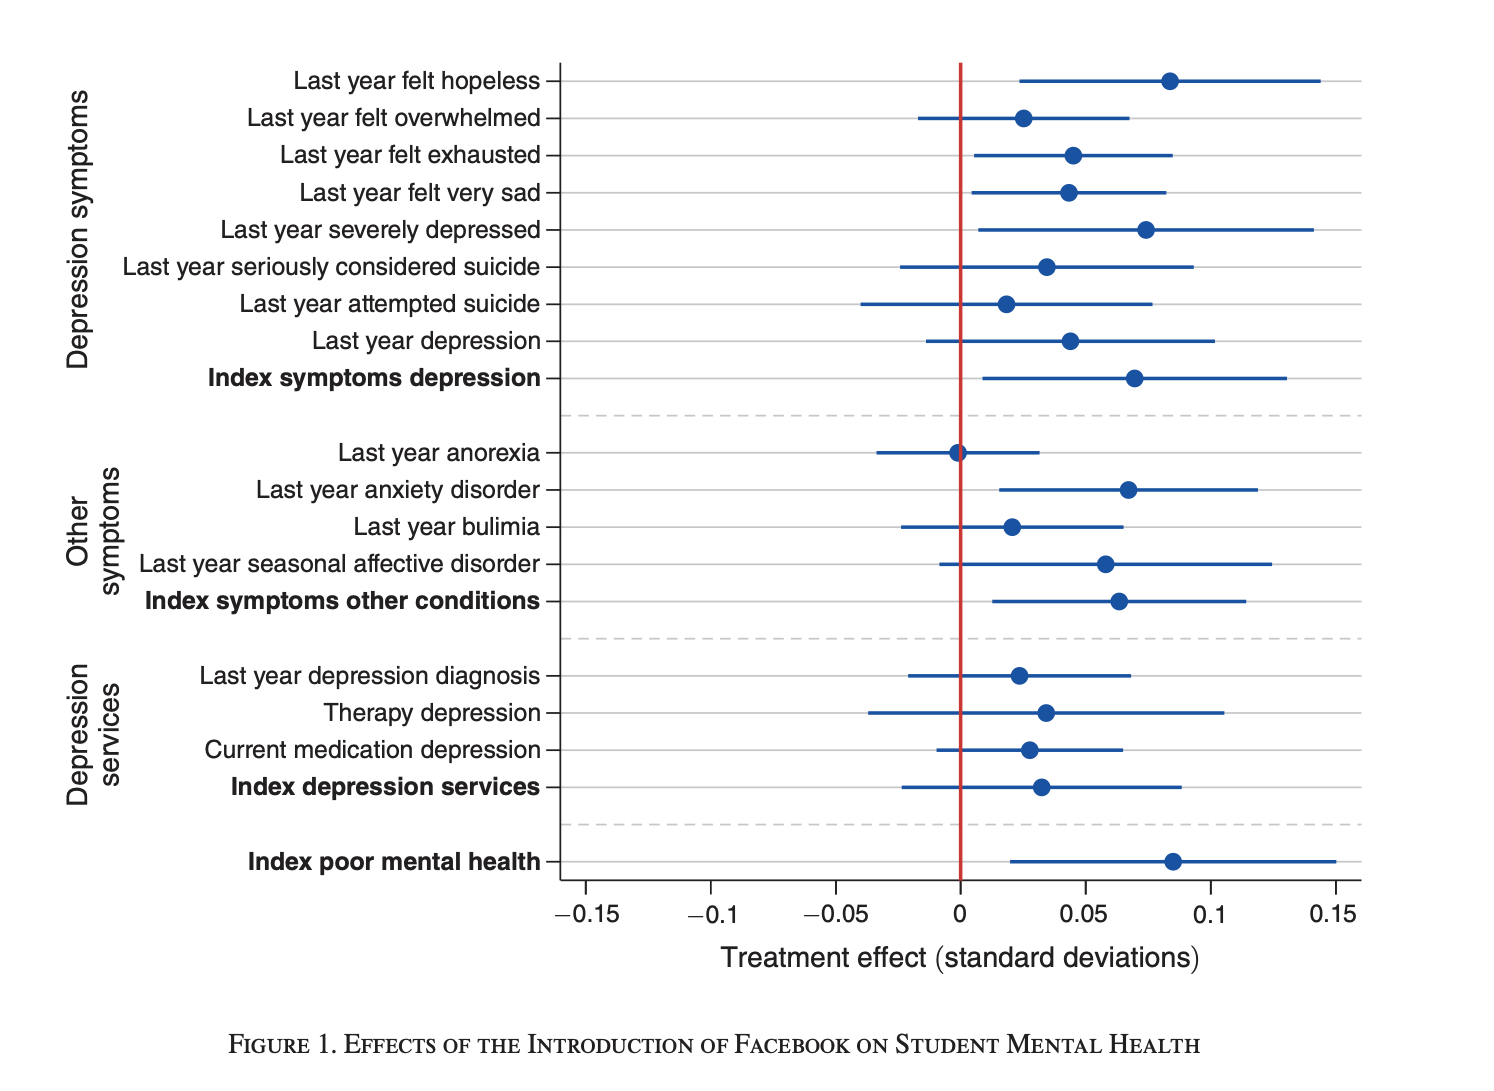
\includegraphics[scale=0.35]{./lecture_includes/facebook_2}
\end{center}
\end{frame}

\begin{frame}
\begin{center}
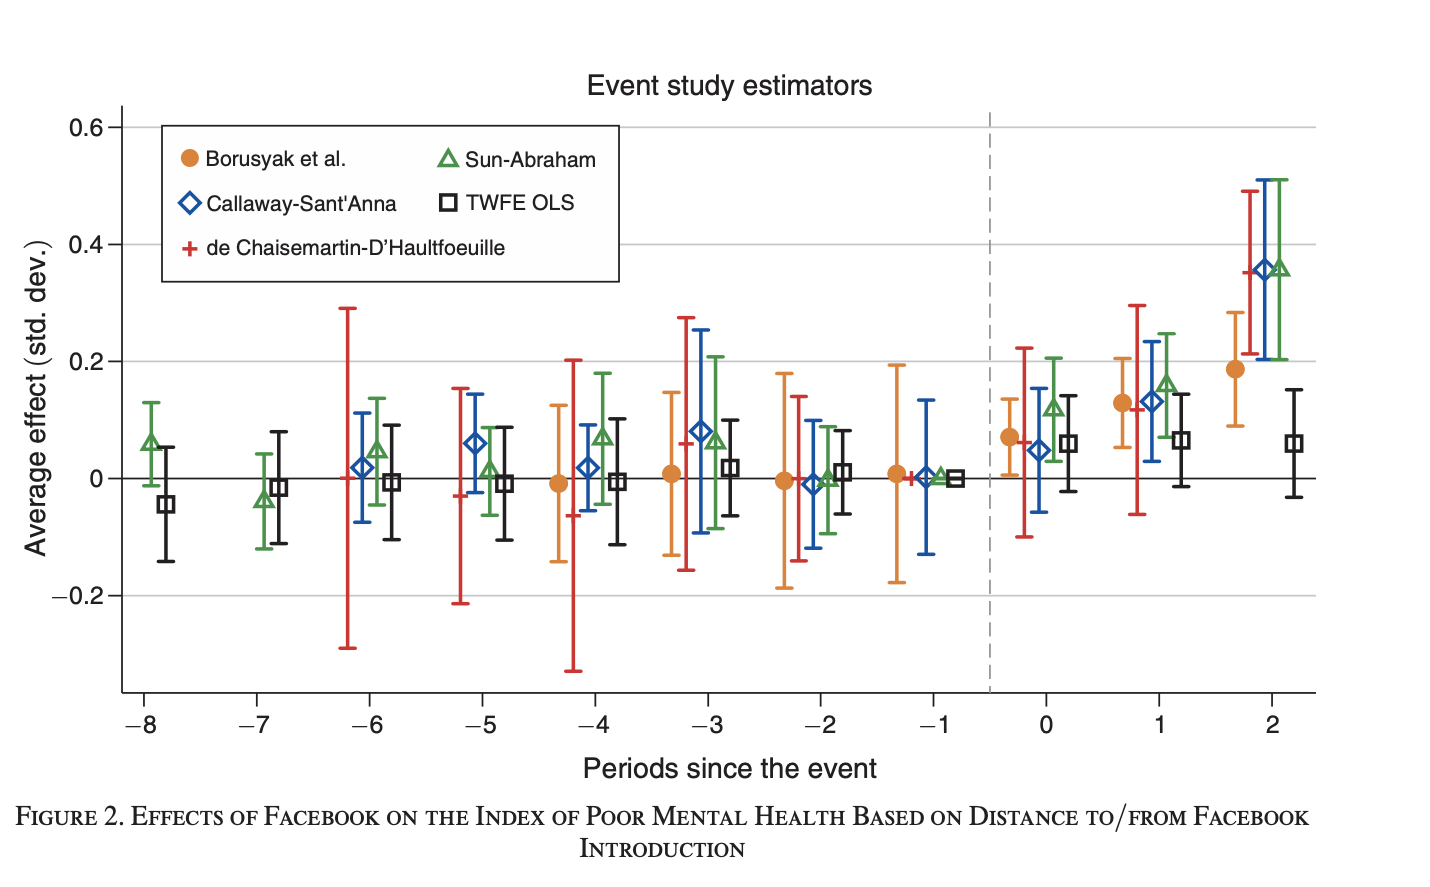
\includegraphics[scale=0.35]{./lecture_includes/facebook_3}
\end{center}
\end{frame}

\begin{frame}
\begin{center}
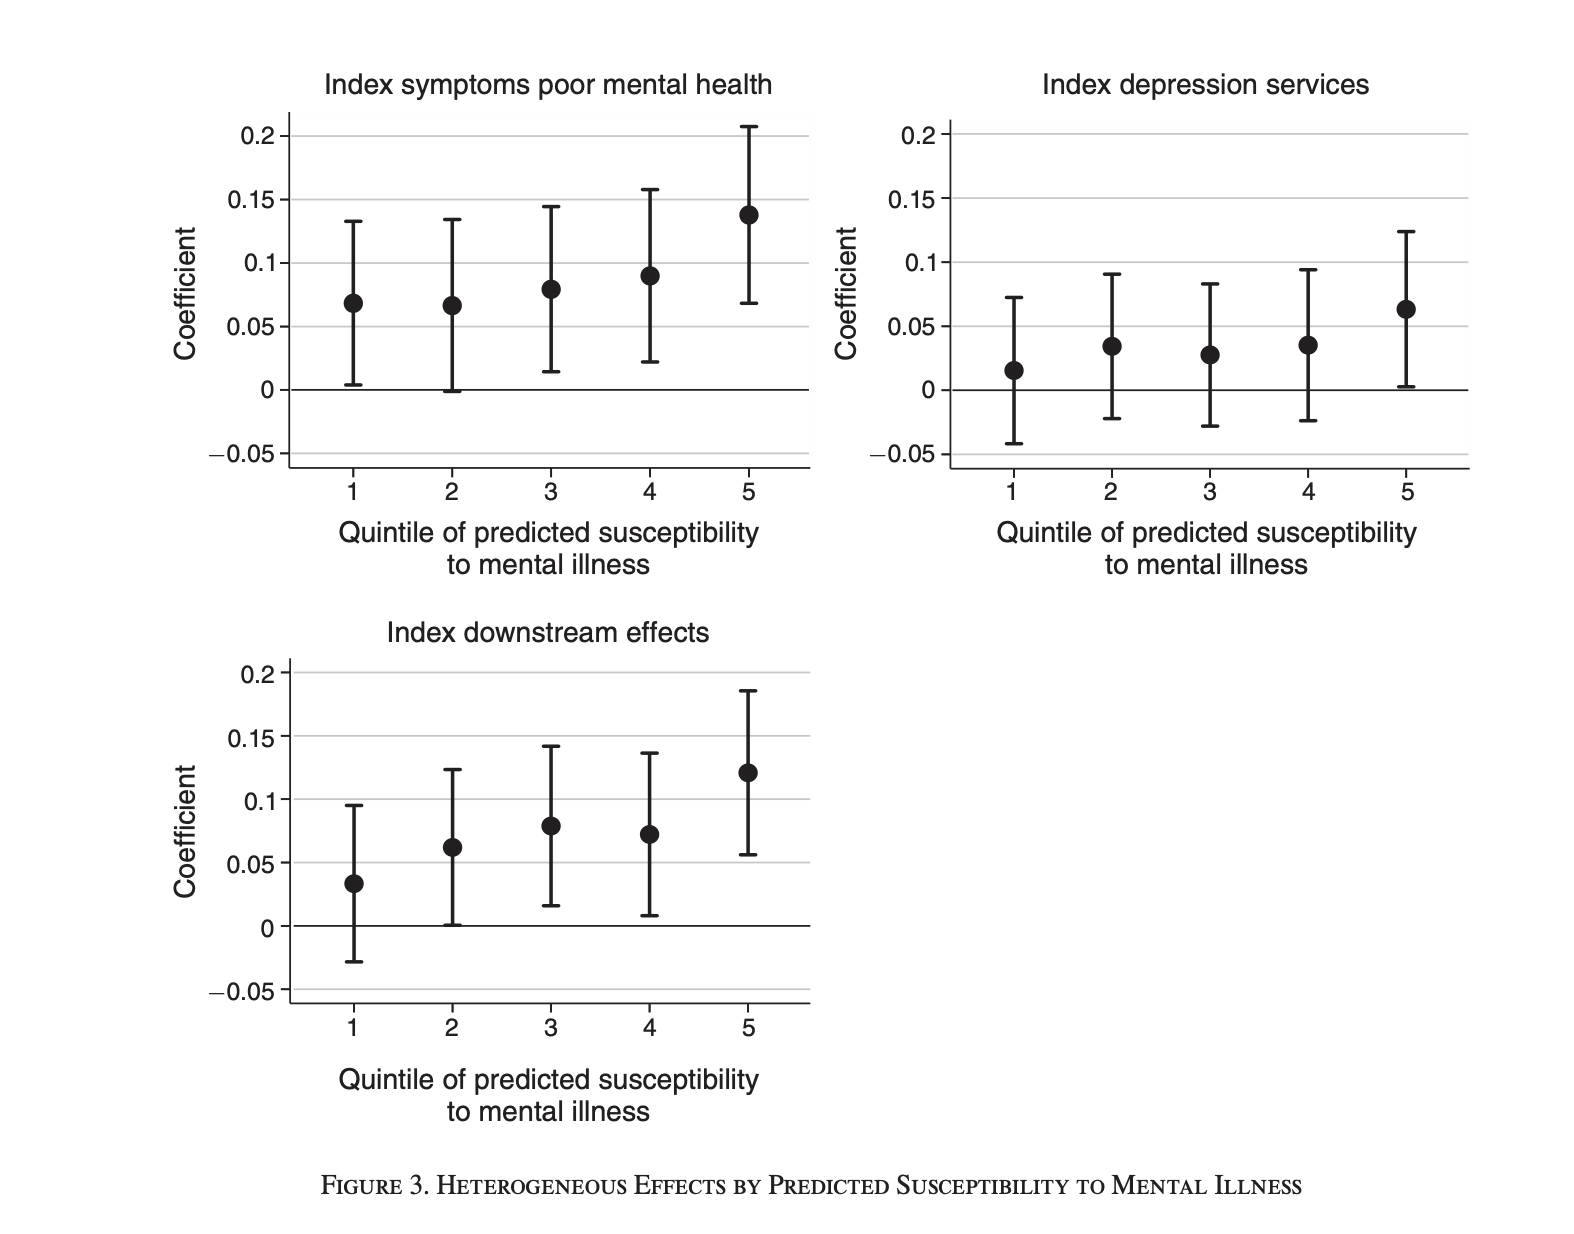
\includegraphics[scale=0.35]{./lecture_includes/facebook_4}
\end{center}
\end{frame}

\begin{frame}
\begin{center}
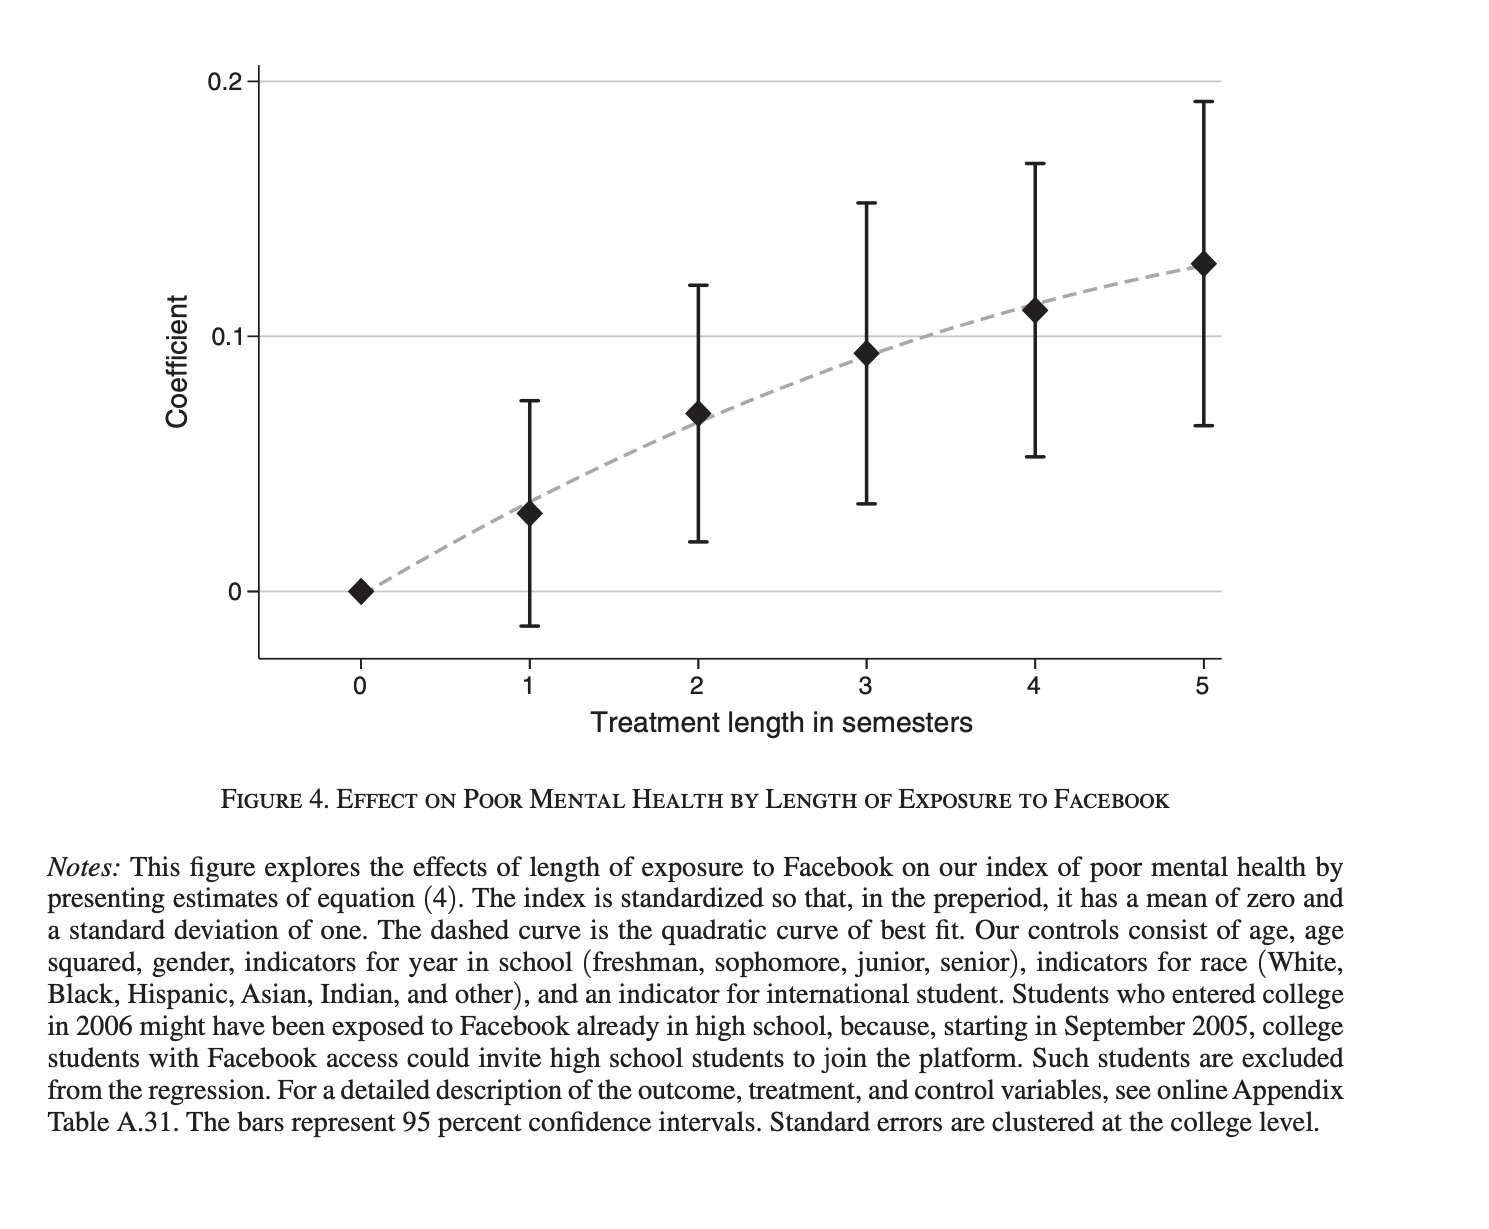
\includegraphics[scale=0.35]{./lecture_includes/facebook_5}
\end{center}
\end{frame}

\begin{frame}
\begin{center}
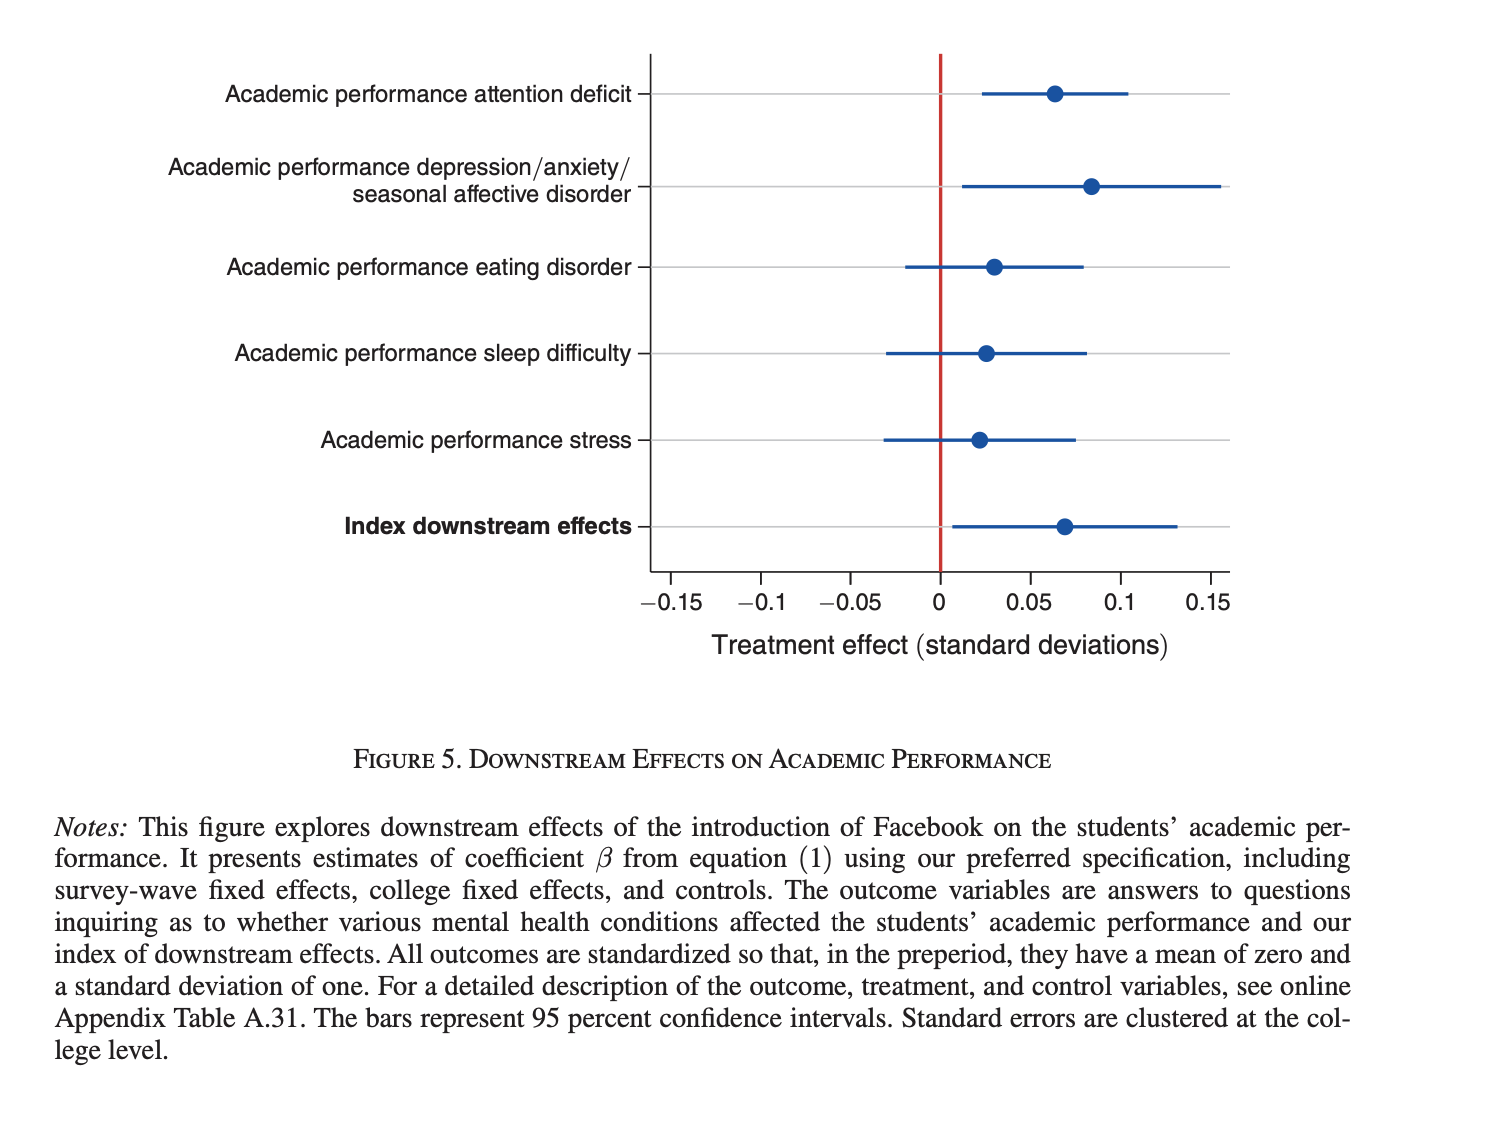
\includegraphics[scale=0.35]{./lecture_includes/facebook_6}
\end{center}
\end{frame}

\begin{frame}
\begin{center}
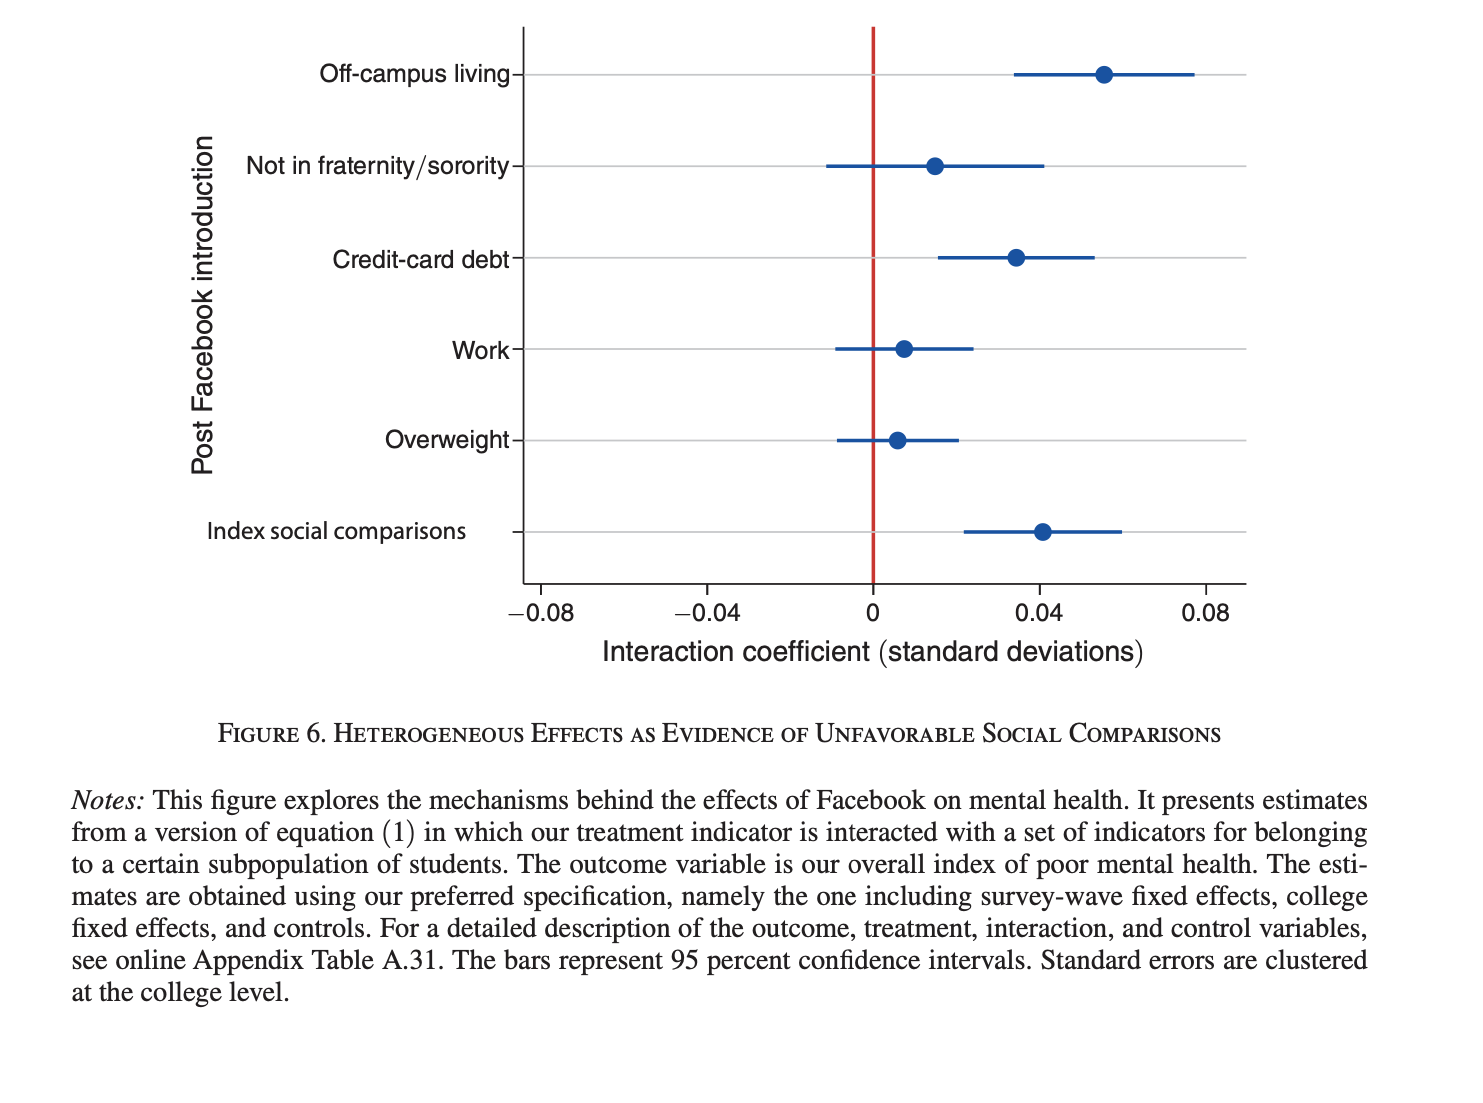
\includegraphics[scale=0.35]{./lecture_includes/facebook_7}
\end{center}
\end{frame}


\begin{frame}{Comments}

\begin{itemize}

\item Can't lose sight of the big picture -- you still have to write a great paper, not just pass your exams, and going from estimation to publishing is a different but related skill
\item Some of the old exhibits may not carry forward (TWFE with many columns)
\item Increasingly, people are presenting a single event study graph with ``all the DiD'' against TWFE so as to avoid cherry picking estimators
\item You should use the tool for the job, but these differences are subtle (``which parallel trends?'', ``which comparison group?'')
\end{itemize}

\end{frame}

\begin{frame}{Conclusion}

\begin{itemize}
\item Good question, good data, and you can publish well with DiD
\item Hardly definitive, but the staggered design is a solution to our inability to run the RCT
\item Remember -- many questions can be randomized in theory but not practice (e.g., smoking)
\item Learn as much as you can and don't stop learning

\end{itemize}

\end{frame}



\section{Synthetic control}
\subsection{Abadie's non-negative weighting}


\begin{frame}[plain]
	\begin{figure}
	\includegraphics[scale=0.25]{./lecture_includes/currie_synth.png}
	\end{figure}
\end{frame}

\begin{frame}{What is synthetic control}
	
	\begin{itemize}
	\item Synthetic control has been called the most important innovation in causal inference of the last two decades (Athey and Imbens 2017)
	\item Originally designed for comparative case studies, but newer developments have extended it to multiple treated units as well as differential timing
	\item Continues to also be methodologically a frontier for applied econometrics, so consider this talk a starting point for you
	\end{itemize}
\end{frame}
	
\begin{frame}{What is a comparative case study}

\begin{itemize}
\item Comparative case studies compare a single unit to another unit to make causal inference
\item Single treated unit is usually a country, state, firm, etc.
\item Social scientists traditionally tackled them either qualitatively and quantitatively (more traditional economic approach)
\end{itemize}

\end{frame}


\begin{frame}{Qualitative comparative case studies}
	
	\begin{itemize}
	\item In qualitative comparative case studies, the goal might be to reason \emph{inductively} the causal effects of events or characteristics of a single unit on some outcome, oftentimes through logic and historical analysis.  
		\begin{itemize}
		\item Classic example of comparative case study approach is Alexis de Toqueville's \underline{Democracy in America} (but he is regularly comparing the US to France)
		\end{itemize}
	\item Sometimes there may not be an explicit counterfactual, or if there is, it's not principled (subjective researcher decision)
	\item Quantitative claims about causal effects are unlikely -- de Toqueville's won't claim GDP per capita fell \$500 when compared against France
	\end{itemize}
\end{frame}

\begin{frame}{Traditional quantitative comparative case studies}

\begin{itemize}
	\item Traditional quantitative comparative case studies are explicitly causal designs in that there is a treatment and control, usually involving natural experiment on a single aggregate unit
	\item Comparison focuses on the the evolution of an aggregate outcome for the unit affected by the intervention to the evolution of the same \emph{ad hoc} aggregate control group (Card 1990; Card and Krueger 1994)
	\item It'll essentially be diff-in-diff, but it may not use the event study, and the point is the choice of controls is a subset of all possible controls
\end{itemize}

\end{frame}

\begin{frame}{Pros and cons}
	
	\begin{itemize}
	\item Pros:
		\begin{itemize}
		\item Takes advantage of policy interventions that take place at an aggregate level (which is common and so this is useful)
		\item Aggregate/macro data are often available (which may be all we have)
		\end{itemize}
	\item Cons:
		\begin{itemize}
		\item Selection of control group is \emph{ad hoc} -- opens up researcher biases, even unconscious
		\item Standard errors do not reflect uncertainty about the ability of the control group to reproduce the counterfactual of interest
		\end{itemize}
	\end{itemize}
\end{frame}

\begin{frame}{Description of the Mariel Boatlift}
	
	\begin{itemize}
	\item In 1980, Fidel Castro allowed anyone to leave Cuba so long as they did in the fall from the Mariel boat dock.
	\item The Mariel Boatlift brought 100,000 Cubans to Miami which increased the Miami labor force by 7\%
	\item Card (1990) uses the Mariel Boatlift as a natural experiment to measure the effect of a sudden influx of immigrants on unemployment among less-skilled natives
	\item His question was how do inflows of immigrants affect the wages and employment of natives in local US labor markets?
	\item Individual-level data on unemployment from the Current Population Survey (CPS) for Miami and comparison cities
	\end{itemize}
\end{frame}


\begin{frame}[plain]
	\begin{figure}
	\includegraphics[scale=0.25]{./lecture_includes/boatlift2.png}
	\end{figure}
\end{frame}

\begin{frame}[plain]
	\begin{figure}
	\includegraphics[scale=0.25]{./lecture_includes/boatlift3.png}
	\end{figure}
\end{frame}

\begin{frame}[plain]
	\begin{figure}
	\includegraphics[scale=0.25]{./lecture_includes/boatlift4.png}
	\end{figure}
\end{frame}


\begin{frame}{Selecting control groups}

\begin{itemize}

\item His treatment group was low skill workers in Miami since that's where Cubans went
\item But which control group?
\item He chose Atlanta, Los Angeles, Houston, Tampa-St. Petersburg

\end{itemize}

\end{frame}



\begin{frame}{Why these four?}

	\begin{figure}
	\includegraphics[scale=0.25]{./lecture_includes/card_illr.png}
	\end{figure}

\end{frame}

\begin{frame}{Diff-in-diff}
	
	\begin{figure}
	\includegraphics[scale=0.75]{./lecture_includes/abadie_2.pdf}
	\end{figure}
\end{frame}

\begin{frame}{Parallel trends}

\begin{itemize}
\item His estimate is unbiased if the change in $Y^0$ for the comparison cities correctly approximates the unobserved $\textcolor{red}{\Delta Y^0}$ for the treatment group
\item But Card largely focused on covariates, and in a relatively casual way (``similar growth'') and does not report much
\item Black result would have been positive, too, were it not that the comparison cities growth was smaller -- uncertainty about null result being from no effect or arbitrary control group
\end{itemize}

\end{frame}


\begin{frame}{Synthetic Control}
	
	\begin{itemize}
	\item Abadie and Gardeazabal (2003) introduced synthetic control in the AER in a study of a terrorist attack in Spain (Basque) on GDP
	\item Revisited again in a 2010 JASA with Diamond and Hainmueller, two political scientists who were PhD students at Harvard (more proofs and inference)
	\item Basic idea is to use a combination of comparison units as counterfactual for a treated unit where the units are chosen according to a data driven procedure
	\end{itemize}
\end{frame}


\begin{frame}{Researcher's objectives}

\begin{itemize}
	\item Our goal here is to reproduce the counterfactual of a treated unit by finding the combination of untreated units that best resembles the treated unit \emph{before} the intervention in terms of the values of $k$ relevant covariates (predictors of the outcome of interest)
	\item Method selects \emph{weighted average of all potential comparison units} that best resembles the characteristics of the treated unit(s) - called the ``synthetic control''
\end{itemize}

\end{frame}

\begin{frame}{Synthetic control method: advantages}
	
	\begin{itemize}
	\item ``Convex hull'' means synth is a weighted average of units which means the counterfactual is a collection of comparison units that on average track the treatment group over time.
	\item Constraints on the model use non-negative weights which does not allow for extrapolation 
	\item Makes explicit the contribution of each comparison unit to the counterfactual 
	\item Formalizing the way comparison units are chosen has direct implications for inference
	\end{itemize}
\end{frame}



\begin{frame}{Notation and setup}
	
Suppose that we observe $J+1$ units in periods $1, 2, \dots, T$
		\begin{itemize}
		\item Unit ``one'' is exposed to the intervention of interest (that is, ``treated'') during periods $T_0+1, \dots, T$
		\item The remaining $J$ are an untreated reservoir of potential controls (a ``donor pool'')
		\end{itemize}	
\end{frame}



\begin{frame}{Group-time ATT with only one treated group}

Using same potential outcomes notation as we've been using, define the ATT parameter as a dynamic group-time

\begin{eqnarray*}
\delta_{1t}&=&Y_{1t}^1 - Y_{1t}^0 \\
&=& Y_{1t} - Y_{1t}^0 
\end{eqnarray*} for each post-treatment period, $t>T_0$ and $Y_{1t}$ is the outcome for unit one at time $t$. We will estimate $Y^0_{1t}$ using the $J$ units in the donor pool 

\end{frame}

\begin{frame}{Estimating W weights}
	
	\begin{itemize}
	\item Let $W=(w_2, \dots, w_{J+1})'$ with $w_j\geq 0$ for $j=2, \dots, J+1$ and $w_2+\dots+w_{j+1}=1$. Each value of $W$ represents a potential synthetic control
	\item Let $X_1$ be a $(k\times 1)$ vector of pre-intervention characteristics for the treated unit.  Similarly, let $X_0$ be a $(k\times J)$ matrix which contains the same variables for the unaffected units.
	\item The vector $W^*=(w_2^*, \dots, w_{J+1}^*)'$ is chosen to minimize $||X_1-X_0W||$, subject to our weight constraints
	\end{itemize}
\end{frame}

\begin{frame}{Donor weights and characteristic weights}
	
Abadie, et al. consider $$||X_1 - X_0W||=\sqrt{(X_1-X_0W)'V(X_1-X_0W)}$$where $X_{jm}$ is the value of the $m$-th covariates for unit $j$ and $V$ is some $(k\times k)$ symmetric and positive semidefinite matrix



\end{frame}

\begin{frame}{More on the V matrix}

Typically, $V$ is diagonal with main diagonal $v_1, \dots, v_k$.  Then, the synthetic control weights $w_2^*, \dots, w_{J+1}^*$ minimize: $$\sum_{m=1}^k v_m \bigg(X_{1m} - \sum_{j=2}^{J+1}w_jX_{jm}\bigg)^2$$ where $v_m$ is a weight that reflects the relative importance that we assign to the $m$-th variable when we measure the discrepancy between the treated unit and the synthetic controls

\end{frame}



\begin{frame}{How this works}

This method of ``minimizing pre-treatment characteristics'' is very similar to nearest neighbor matching from Abadie and Imbens (2006)

\bigskip

Let's look at it together; it should help you understand, too, the idea of the V matrix being crucial

\bigskip

\url{https://docs.google.com/spreadsheets/d/1iro1Qzrr1eLDY_LJVzOYvnQZWmxY8JyTcDf6YcdhkwQ/edit?usp=sharing}

\end{frame}

\begin{frame}{Donor weights and characteristic weights}

\begin{itemize}
\item If all pre-treatment characteristics are treated equally, then there exists a solution to the minimization, $W^*$
\item But if pre-treatment characteristics were emphasized differently in the minimization (say one was given a weight of 0.00001), then there is a different solution, $W*'$.
\item Making a choice about $V$ (the weight on pre-treatment characteristics' importance) is unavoidable -- a non-choice is a choice as you'll just weight all characteristics the same
\end{itemize}

\end{frame}


\begin{frame}{Keeping in mind our goal - create a good synth}
	
		\begin{itemize}
		\item The synthetic control $W^*(V^*)$ is meant to reproduce the behavior of the outcome variable for the treated unit in the absence of the treatment
		\item Therefore, the $V^*$ weights directly shape $W^*$
		\end{itemize}
\end{frame}

\begin{frame}{Estimating the $V$ matrix}
	
 Choice of $v_1, \dots, v_k$ can be based on
		\begin{itemize}
		\item Assess the predictive power of the covariates using regression
		\item Subjectively assess the predictive power of each of the covariates, or calibration inspecting how different values for $v_1, \dots, v_k$ affect the discrepancies between the treated unit and the synthetic control
		\item Minimize mean square prediction error (MSPE) for the pre-treatment period (default):
			\begin{eqnarray*}
			\sum_{t=1}^{T_0} \bigg(Y_{1t} - \sum_{j=2}^J w_j^*(V^*)Y_{jt} \bigg)^2
			\end{eqnarray*}
		\end{itemize}
\end{frame}

\begin{frame}{Choosing pre-treatment characteristics}

\begin{itemize}
\item Original papers provided no guidance, and it's unclear how these characteristics connect to the factor model
\item Goal is over a long stretch pre-treatment to create the convex hull that contains the treatment group
\item Lots of early variation in what was done (including my papers), and some effort has now been made to be more principled to avoid p-hacking
\end{itemize}

\end{frame}

\begin{frame}{Cross validation}

Abadie suggests model selection using specifications guided by sample splitting into training and validation:

\begin{itemize}
		\item Divide the pre-treatment period into an initial \textbf{training} period and a subsequent \textbf{validation} period
		\item For any given $V$, calculate $W^*(V)$ in the training period.
		\item Minimize the MSPE of $W^*(V)$ in the validation period
\end{itemize}

\end{frame}


\begin{frame}{Avoiding Cherry Picking Synth}

Ferman, Pinto and Possbaum (2020) note that there are opportunities for p-hacking in model selection and recommend reporting a variety of specifications rather than just one

\begin{enumerate}
\item Use all pre-treatment lagged outcomes as your $X$ characteristics
\item Use first three-fourths
\item Use first half
\item Use all odd years
\item Use all even years
\item Use pre-treatment outcome mean
\item Use three outcome values
\end{enumerate}

\bigskip

With and without covariates, report p-values (explained later) and event study plot

\end{frame}

\begin{frame}{14 specification p-values}

	\begin{figure}
	\includegraphics[scale=0.5]{./lecture_includes/cherry_picking_1.png}
	\end{figure}

\end{frame}

\begin{frame}{14 specification event studies}

	\begin{figure}
	\includegraphics[scale=0.5]{./lecture_includes/cherry_picking_2.png}
	\end{figure}

\end{frame}


\begin{frame}{Synth identification}

\begin{itemize}
\item In diff-in-diff, the core assumption was parallel trends
\item Only needed one pretreatment period for identification but needed parallel trends starting at that period
\item Synthetic control does not use parallel trends for identification; it uses a factor model of $Y^0$
\item But you need a long pre-treatment series, not just for the event study, but for modeling the heterogeneity adequately
\end{itemize}

\end{frame}


\begin{frame}{Assumption: $Y^0$ is determined by factor model}

What about unmeasured factors affecting the outcome variables as well as heterogeneity in the effect of observed and unobserved factors?
\begin{eqnarray*}
Y_{it}^0 = \alpha_t + \theta_t Z_i + \lambda_t u_i + \varepsilon_{it}
\end{eqnarray*}where $\alpha_t$ is an unknown common factor with constant factor loadings across units, and $\lambda_t$ is a vector of unobserved common factors

\end{frame}

\begin{frame}{With some manipulation}

\begin{eqnarray*}
Y^0_{1t} - \sum^{J+1}_{j=2}w^*_jY_{jt} &=& \sum_{j=2}^{J+1} w_j^* \sum_{s=1}^{T_0} \lambda_t \bigg ( \sum_{n=1}^{T_0} \lambda_n'\lambda_n \bigg )
^{-1} \lambda_s'(\varepsilon_{js} - \varepsilon_{1s} ) \\
&& - \sum_{j=2}^{J+1} w_j^* (\varepsilon_{jt} - \varepsilon_{1t})
\end{eqnarray*}

\begin{itemize}
\item If $\sum_{t=1}^{T_0} \lambda_t' \lambda_t$ is nonsingular, then RHS will be close to zero if number of preintervention periods is ``large''  relative to size of transitory shocks 
\item Only units that are alike in observables and unobservables should produce similar trajectories of the outcome variable over extended periods of time
\item Main takeaway: you need a long pre-treatment time period to use this and the fit must be excellent
\end{itemize}


\end{frame}


\begin{frame}{Example: California's Proposition 99}
	
	\begin{itemize}
	\item In 1988, California first passed comprehensive tobacco control legislation:
		\begin{itemize}
		\item increased cigarette tax by 25 cents/pack
		\item earmarked tax revenues to health and anti-smoking budgets
		\item funded anti-smoking media campaigns
		\item spurred clean-air ordinances throughout the state
		\item produced more than \$100 million per year in anti-tobacco projects
		\end{itemize}
	\item Other states that subsequently passed control programs are excluded from donor pool of controls (AK, AZ, FL, HI, MA, MD, MI, NJ, OR, WA, DC)
	\end{itemize}
\end{frame}

\begin{frame}{Cigarette Consumption: CA and the Rest of the US}
	
	\begin{figure}
	\includegraphics[scale=0.75]{./lecture_includes/abadie_3.pdf}
	\end{figure}
\end{frame}

\begin{frame}{Cigarette Consumption: CA and synthetic CA}
	
	\begin{figure}
	\includegraphics[scale=0.75]{./lecture_includes/abadie_4.pdf}
	\end{figure}
\end{frame}

\begin{frame}{Predictor Means: Actual vs. Synthetic California}
	
	\begin{figure}
	\includegraphics[scale=0.75]{./lecture_includes/abadie_5.pdf}
	\end{figure}
\end{frame}

\begin{frame}{Smoking Gap between CA and synthetic CA}
	
	\begin{figure}
	\includegraphics[scale=0.75]{./lecture_includes/abadie_6.pdf}
	\end{figure}
\end{frame}

\begin{frame}{Inference}
	
	\begin{itemize}
	\item To assess significance, we calculate exact p-values under Fisher's sharp null using a test statistic equal to after to before ratio of RMSPE
	\item Exact p-value method
		\begin{itemize}
		\item Iteratively apply the synthetic method to each country/state in the donor pool and obtain a distribution of placebo effects
		\item Compare the gap (RMSPE) for California to the distribution of the placebo gaps. For example the post-Prop. 99 RMSPE is: 
			\begin{eqnarray*}
			RMSPE = \bigg(\frac{1}{T-T_0} \sum_{t=T_0+1}^T \bigg(Y_{1t} - \sum_{j=2}^{J+1} w_j^* Y_{jt}\bigg)^2 \bigg)^{\frac{1}{2}}
			\end{eqnarray*}and the exact p-value is the treatment unit rank divided by $J$
		\end{itemize}
	\end{itemize}
\end{frame}

\begin{frame}{Smoking Gap for CA and 38 control states}
	
	\begin{figure}
	\includegraphics[scale=0.75]{./lecture_includes/abadie_7.pdf}
	\end{figure}
\end{frame}

\begin{frame}{Smoking Gap for CA and 34 control states}
	
	\begin{figure}
	\includegraphics[scale=0.75]{./lecture_includes/abadie_8.pdf}
	\end{figure}
\end{frame}

\begin{frame}{Smoking Gap for CA and 29 control states}
	
	\begin{figure}
	\includegraphics[scale=0.75]{./lecture_includes/abadie_9.pdf}
	\end{figure}
\end{frame}

\begin{frame}{Smoking Gap for CA and 19 control states}
	
	\begin{figure}
	\includegraphics[scale=0.75]{./lecture_includes/abadie_10.pdf}
	\end{figure}
\end{frame}

\begin{frame}{Ratio Post-Prop. 99 RMSPE to Pre-Prop. 99 RMSPE}

	\begin{figure}
	\includegraphics[scale=0.75]{./lecture_includes/abadie_11.pdf}
	\end{figure}
\end{frame}



\begin{frame}{Example}

\begin{itemize}

\item Let's look at an example now from my own work
\item Rhode Island legalized sex work in 1980 (indoor anyway) but did so accidentally
\item Judge enforced it in 2003
\item Use DiD and synth to estimate the effect on violence and STIs
\item Also bite and mechanism
\end{itemize}

\end{frame}

\begin{frame}{Institutional details}

\begin{itemize}
	\item Google alert in 2009 took me to an article that told this whole story
	\item There is no evidence that anyone knew about the 1980 legalization
	\item Appears to be unintentional legalization due to poorly worded amendments to \S 11-34
	\item  July/August 2003 ``Operation Rubdown'' and judicial decriminalization
		\begin{itemize}
		\item Wave of arrests of massage parlor employees.
		\item Judge dismisses charges against massage parlor employees and police stop arresting indoor sex workers
		\end{itemize}
\end{itemize}

\end{frame}


\begin{frame}{``Accidental'' and unknown legalization}

		\begin{itemize}
		\item Senator John Revens Jr. (2009) on the 1980 General Assembly
			\begin{itemize}
			\item ``they would never sponsor a bill decriminalizing prostitution if they knew what it was.  No way.  Not in a million years'' (Arditi 2009)
			\end{itemize}
		\item Senator John F. McBurney III (from the 1980 GA) 
			\begin{itemize}
			\item ``We probably vote on 500 bills a year.  \dots Legislators didn't know what they were voting for.''
			\end{itemize}
		\item Unusual lack of awareness of the 1980 law from 1980--2005
			\begin{itemize}
			\item Not a single mention of the law change in any newspaper until Breton (2005)
			\item No legal scholars mention it (e.g., Posner and Silberbaugh 1996)
			\end{itemize}
		\end{itemize}

\end{frame}


\begin{frame}{Discovery of Loophole}
	\begin{itemize}
	\item 1997 \emph{State vs. DeMagistris}:  \S 11-34-8 and \S 11-34-8.1 apply only to street prostitution
	\item  July/August 2003 ``Operation Rubdown'' and judicial decriminalization
		\begin{itemize}
		\item Wave of arrests of massage parlor employees.
		\item Judge dismisses charges against massage parlor employees and police stop arresting indoor sex workers
		\end{itemize}
	\end{itemize}
\end{frame}


\begin{frame}{Learning}
	\begin{itemize}
		\item Police stop arresting indoor sex workers
		\bigskip
		
		\begin{quote}``Chief of Police Tom Verdi says that until 2 years ago, Providence police were arresting alleged prostitutes inside massage parlors.  But they stopped doing so after [Kiselica] persuaded District Court judges to dismiss prostitution cases \emph{based on the wording of the current law}.'' (2005 newspaper article)
		\end{quote}
		
%		\item Kiselica begins advises Korean community
		\item Re-criminalization in 2009
	\end{itemize}
\end{frame}

\begin{frame}{Our study}

\begin{itemize}
\item Tons of evidence that sex workers are raped at a higher rate than the general population
\item Tons of evidence that sex workers have been the drivers of STI epidemics in areas
\item But is this causal, or is it correlational?
\item And is this caused by sex work or is it caused by sex work policy?
\item We didn't know -- humility! -- until this study
\end{itemize}

\end{frame}


\begin{frame}{Proposed Mechanism Framework: Rape}
\begin{enumerate}
  \item Decriminalization $\Uparrow$ rape offenses:
  \begin{itemize}
    \item Increase number transactions in indoor sex market by reducing costs of indoor sex work $\Rightarrow$ increase prostitution related violence 
  \end{itemize}
  \item Decriminalization $\Downarrow$ rape offenses:
 \begin{itemize}
   \item Freeing up of police personnel and resources
  \item Firms invest in locks, security cameras, security personnel to reduce opportunity of premeditated client violence \begin{footnotesize}(Brents and Hausbeck 2005)\end{footnotesize}
  \item Sex workers more willing to cooperate with police/less police abuse \begin{footnotesize}(Church et al. 2001, Levitt and Venkatesh, 2007)\end{footnotesize}
   \item Could reduce male violence if prostitution is substitute for violence against women \begin{footnotesize}(Posner 1994)\end{footnotesize}

\end{itemize}
\end{enumerate}
\end{frame}


\begin{frame}{Proposed Mechanism Framework: STIs}
\begin{enumerate}
  \item Decriminalization $\Uparrow$ population STIs:
  \begin{itemize}
    \item Increase number transactions in indoor sex market $\Rightarrow$ increase the scale and growth rate of a gonorrhea epidemic 
  \end{itemize}
  \item Decriminalization $\Downarrow$ population STIs:
 \begin{itemize}
  \item If decriminalization shifts transactions indoors to lower STI risk sex workers and/or draws in lower risk sex workers $\Rightarrow$ decrease an epidemic \begin{footnotesize}(Kremer 1996)\end{footnotesize}
  \item \begin{footnotesize}Empirical evidence of safer indoor sex work:\end{footnotesize}
   \begin{itemize}
   \item \begin{footnotesize} More indoor transactions (relative to street) lower STI rates \begin{scriptsize}(Gertler and Shah 2011)\end{scriptsize}
   \item  Massage parlor SWs in UK use condoms more, receive STI screens more, report fewer weekly transaction than street-based SWs \begin{scriptsize}(Jeal and Salisbury 2007)\end{scriptsize}
       \item  Higher gonorrhea incidence and more requests for non-condom sex among illegal street SWs than licensed indoor SWs in Australia \begin{scriptsize}(Seib et al. 2009)\end{scriptsize}\end{footnotesize}
\end{itemize}
  \end{itemize}
\end{enumerate}
\end{frame}





%\begin{frame}[shrink=20]{Synthetic Control Model: Rape}
%\begin{figure}
%\includegraphics{./lecture_includes/rape_synthetic.pdf}
%\end{figure}
%\end{frame}



%\begin{frame}[shrink=20]{Synthetic Control Female Gonorrhea}
%\begin{figure}
%\includegraphics{./lecture_includes/synth_gon.pdf}
%\end{figure}
%\end{frame}




\begin{frame}{We collected a lot of different data}
\begin{itemize}
	\item Lots of crime data (from the FBI from police)
	\item Lots of data on gonorrhea (from the CDC)
	\item Lots of data on classified ads for massage parlors (from the Providence Phoenix)
	\item Lots of data on prostitution arrests (from the FBI from police)
	\item Lots of data on indoor sex workers reviewed online by clients (from The Erotic Review)
\end{itemize}
\end{frame}

\begin{frame}{Evidence}

\begin{enumerate}
\item \textbf{Bite}: Advertising and sex worker reviews
\item \textbf{Falsifications}: Other crimes
\item \textbf{Mechanism}: Entry and sex acts
\item \textbf{Main results}: DiD and synth estimates of ATT for rape and gonorrhea
\item \textbf{Visuals}: Lots of event study and synth plots
\end{enumerate}

\end{frame}


\begin{frame}[shrink=20]{Providence Phoenix Advertising}
	\begin{figure}
	\includegraphics[totalheight=0.95 \textheight]{./lecture_includes/phx_ndx.pdf}
	\end{figure}
\end{frame}


\begin{frame}[shrink=20]{Providence Phoenix Advertising (Before)}
	\begin{figure}
	\includegraphics[totalheight=0.95 \textheight]{./lecture_includes/spa_jan03.jpg}
	\end{figure}
\end{frame}


\begin{frame}[shrink=20]{Providence Phoenix Advertising (After)}
	\begin{figure}
	\includegraphics[totalheight=0.95 \textheight]{./lecture_includes/spa_july04.jpg}
	\end{figure}
\end{frame}

% Quantities and prices
\begin{frame}{Market Prices and Composition}
	\begin{figure}
	\includegraphics[scale=0.4]{./lecture_includes/table3.pdf}
	\end{figure}
Prices fell, number of massage sex workers rose, risky sex fell, and number of asian sex workers rose
\end{frame}

\clearpage
\newpage


\begin{frame}{Arrests, rapes and gonorrhea}
So it looks like the policy caused sex work to increase -- itself new, as many don't think it can change

\bigskip

But Gary Becker (Rest in Peace) said our goal needs to be to minimize the social costs of crime -- so did this policy increase or decrease those social costs?

\bigskip

Let's look at sex worker arrests, rapes, and gonorrhea

\bigskip

Causal assumption: if what happens in other states is what \emph{would have happened}  (``parallel trends'') in Rhode Island, then we can use the other states as substitutes for Rhode Island counterfactuals

\end{frame}



\begin{frame}[shrink=20]{Parallel trends: prostitution arrests}
	\begin{figure}
	\includegraphics[scale=0.35]{./lecture_includes/figure2c.pdf}
	\end{figure}
\end{frame}

\begin{frame}[shrink=20]{Parallel trends: rape offenses}
	\begin{figure}
	\includegraphics[scale=0.35]{./lecture_includes/figure2a.pdf}
	\end{figure}
\end{frame}

\begin{frame}[shrink=20]{Parallel trends: gonorrhea offenses}
	\begin{figure}
	\includegraphics[scale=0.35]{./lecture_includes/figure2b.pdf}
	\end{figure}
\end{frame}


\clearpage




\begin{frame}[shrink=20]{Arrests, Rapes and Gonorrhea}
	\begin{figure}
	\includegraphics[scale=0.35]{./lecture_includes/table2.pdf}
	\end{figure}
\end{frame}



\begin{frame}{Synthetic Control Analysis}\label{weights}
\begin{itemize}
\item Think about minimum wage increases -- they happen in different places at different points in time
\item Synthetic control estimator is useful when only one group is treated at one point in time
\item Similar to what we did only 1) we don't need parallel trends anymore and 2) only uses the best states as controls
\item What's the best states?  The ones that had the same time path in rapes, gonorrhea and arrests before the legalization event
\item ``If they looked the same before, why wouldn't they look the same after?''
\end{itemize}

\end{frame}


\begin{frame}[shrink=20]{Synthetic Control Model: Rape}
\begin{figure}
\includegraphics[scale=1.25]{./lecture_includes/raperate_synthetic.pdf}
\end{figure}
\end{frame}

\begin{frame}[shrink=20]{Synthetic Control Female Gonorrhea}\label{sc_femgon}
\begin{figure}
\includegraphics{./lecture_includes/synth_gonorrhea_estimate}
\end{figure}
\end{frame}



\begin{frame}{Why did reported female rape offenses fall?}

Some possible explanations

\begin{enumerate}
  \item Did police reallocate resources away from arrests to investigating rapist? Defense attorney told us \textbf{no}
  \item Did definitions of rape change?  \textbf{Not at this time}
  \item Did fewer sex workers get raped after decriminalization? Probably but most \emph{reported} rapes \textbf{are not} sex workers in the first place
  \item Did violent males think of rape and sex with prostitutes as substitutes?  \textcolor{red}{Maybe?}
\end{enumerate}
\end{frame}



\begin{frame}{Why did female gonorrhea rates fall?}

Some possible explanations

\begin{enumerate}
  \item Safer sex workers entered the market thus diluting the propagation of gonorrhea 
  \item Safer sex in relevant part of sexual network thus diluting the propagation of gonorrhea
  \item Spillovers to males causing feedbacks throughout the network
\end{enumerate}
\end{frame}

\begin{frame}{Compositional effects}
	\begin{figure}
	\includegraphics[scale=0.4]{./lecture_includes/table3.pdf}
	\end{figure}
\end{frame}

\begin{frame}{Spillovers}
	\begin{figure}
	\includegraphics[scale=0.65]{./lecture_includes/table6a.pdf}
	\end{figure}
\end{frame}


\begin{frame}{Recriminalization}

	\begin{itemize}
	\item November 2009: sweeping sex trafficking legislation
	\item Prostitution in all its forms (including indoor) recriminalized
	\end{itemize}
\end{frame}

\begin{frame}{Market Prices and Composition}
	\begin{figure}
	\includegraphics[scale=0.4]{./lecture_includes/table7.pdf}
	\end{figure}
\end{frame}

\begin{frame}[shrink=20]{Recriminalization: Arrests}
	\begin{figure}
	\includegraphics[scale=1]{./lecture_includes/eclplot_2012_pro_2.pdf}
	\end{figure}
\end{frame}

\begin{frame}[shrink=20]{Recriminalization: Rape Offenses}
	\begin{figure}
	\includegraphics[scale=1]{./lecture_includes/eclplot_2012_rape_2.pdf}
	\end{figure}
\end{frame}

\begin{frame}[shrink=20]{Recriminalization: Gonorrhea}
	\begin{figure}
	\includegraphics[scale=1]{./lecture_includes/eclplot_2012_lngon_2}
	\end{figure}
\end{frame}





\begin{frame}{Coding exercise}
	
	\begin{itemize}
	\item The US has the highest prison population of any OECD country in the world 
	\item 2.1 million are currently incarcerated in US federal and state prisons and county jails
	\item Another 4.75 million are on parole
	\item From the early 1970s to the present, incarceration and prison admission rates quintupled in size
	\end{itemize}
\end{frame}



\begin{frame}[plain]

\begin{figure}
\includegraphics[scale=0.5]{./lecture_includes/cook2010.pdf}
\end{figure}
\end{frame}


\begin{frame}{Prison constraints}

	
	\begin{itemize}
	\item Prisons are and have been at capacity for a long time so growth in imprisonment would bite on state corrections
	\item Managing increased flows can only be solved by the following:
		\begin{itemize}
		\item Prison construction
		\item Overcrowding
		\item Paroles
		\end{itemize}
	\item Texas chooses overcrowding
	\end{itemize}
\end{frame}



\begin{frame}{Ruiz v. Estelle 1980}

	
	\begin{itemize}
		\item Class action lawsuit against TX Dept of Corrections (Estelle, warden). 
		\item TDC lost.  Lengthy period of appeals and legal decrees.  
		\item Lengthy period of time relying on paroles to manage flows
	\end{itemize}
\end{frame}

\begin{frame}[shrink=30,plain]

\begin{figure}
\includegraphics{./lecture_includes/flow_rate_figure.pdf}
\end{figure}
\end{frame}



\begin{frame}{Texas prison boom}

Governor Ann Richards (D) 1991-1995
		\begin{itemize}
		\item Operation prison capacity increased 30-35\% in 1993, 1994 and 1995. 
		\item Prison capacity increased from 55,000 in 1992 to 130,000 in 1995.  
		\item Building of new prisons (private and public)
		\end{itemize} 
\end{frame}


\begin{frame}[shrink=30,plain]

\begin{figure}
\includegraphics{./lecture_includes/tdcj.pdf}
\end{figure}
\end{frame}


\begin{frame}[shrink=30,plain]
\begin{figure}
\includegraphics{./lecture_includes/capacity_operational_texas.pdf}
\end{figure}
\end{frame}



\begin{frame}[shrink=30,plain]

\begin{figure}
\includegraphics{./lecture_includes/total_incarceration.pdf}
\end{figure}
\end{frame}

\begin{frame}[shrink=30,plain]

\begin{figure}
\includegraphics{./lecture_includes/synth_placebo_totalincarceration1993.pdf}
\end{figure}
\end{frame}





\begin{frame}{Coding together}

\begin{itemize}
\item Let's go to Mixtape Sessions repository now into /Labs/Texas 
\item I'll walk us through the Stata and R code so you understand the syntax and underlying logic
\item But then I have us a practice assignment 
\end{itemize}

\end{frame}


\begin{frame}{Last Comments}

\begin{itemize}

\item Synthetic control has opponents
\item One criticism is people will say the weights are implausible
\item But that's because they have their own ``mental synth'' model that tells them what weights should or shouldn't be
\item Tell story about conference where Abadie presented Germany paper
\item Synth tells you the weights; OLS you have to calculate them and no one does

\end{itemize}

\end{frame}

\begin{frame}{Regression vs synth weights}
	\begin{figure}
	\includegraphics[scale=0.5]{./lecture_includes/abadie2015_table1.png}
	\end{figure}
\end{frame}

\begin{frame}{Where to now?}

\begin{itemize}

\item So synth is rising as we saw in the figure
\item And developments in diff in diff maybe have lowered the \emph{relative price} of using synth by making them not terribly different
\item But the positive weights has been an issue for some who want extrapolation
\item Let's look at that now

\end{itemize}

\end{frame}


\subsection{Ben-Michael, et al's Least Negative Weighting Method}

\begin{frame}{Introducing Augmented Synthetic Control}
\begin{itemize}
\item Synthetic control has built in constraints forcing weights to be non-negative
\item Convex hull constraint ensures that synth is a feasible counterfactual in that it is formed by a combination of control units similar on pre-intervention characteristics
\item Improves the validity of the estimated effect as there exists interpolated comparison group; similar to common support concept
\item But, the convex hull constraint reduces extrapolation bias from comparing dissimilar units, but at the cost of failing to find matches at all
\end{itemize}

\end{frame}


\begin{frame}

\begin{quote}
``The applicability of the [ADH2010] method requires a sizable number of pre-intervention periods. The reason is that the credibility of a synthetic control depends upon how well it tracks the treated unit’s characteristics and outcomes over an extended period of time prior to the treatment. \textbf{We do not recommend using this method when the pretreatment fit is poor or the number of pretreatment periods is small}. A sizable number of post-intervention periods may also be required in cases when the effect of the intervention emerges gradually after the intervention or changes over time.'' (my emphasis, Abadie, et al. 2015)
\end{quote}

\end{frame}

\begin{frame}{What is augmented synthetic control?}

\begin{itemize}
\item Eli Ben-Michael, Avi Feller and Jesse Rothstein present a modification to ADH in which they allow for negative weights, but only minimally so
\item This model will ``augment'' the original synthetic control model by adjusting for pre-treatment imbalance using doubly robust bias adjustment 
\item Augmentation is conservative; it uses \textbf{penalized ridge regression} but with constraints such that the negative weighting is only to the convex hull, not to the center of the convex hull
\end{itemize}

\end{frame}




\begin{frame}{Gist of their argument}

\begin{enumerate}
\item ADH (``synth'') needs perfect fit and so is biased in practical settings due to the curse of dimensionality as it won't be the case we get weights constrained to be ``on the simplex''
\item Their augmentation will introduce an outcome model to estimate the bias caused by covariate imbalance 
\item Introduces ridge regularization linear regression to estimate new weights to reweight synth
\item Think of it as ``bias reduction'' like Abadie and Imbens (2011) plus it will have doubly robust properties and be equivalent to inverse probability weighting
\item When synth is imbalanced, augmented synth will reduce bias reweighting and bias correction, and when synth is balanced, they are the same
\end{enumerate}

\end{frame}


\begin{frame}{Gist of their argument}

\begin{enumerate}
\item Ridge regularization linear regression used to estimate weights used to reweight the original synth model
\item If synth is imbalanced, augmented synth reducees bias by reweighting and bias correction
\item When synth is balanced, the augmented and original synth are identical (but in practice, they won't be identical)
\item They argue synth DiD can be seen as a special case of augmented synth
\end{enumerate}

\end{frame}


\begin{frame}{Some topical observations}

\begin{itemize}
\item Foregoes estimating \emph{donor pool unit weights} (e.g., ADH, synth did, MCNN)
\item Synth sequels are using penalization/regularization for estimation
\item Relaxes some of the original ADH constraints, like non-negative weights (i.e., no extrapolation)
	\begin{itemize}
	\item This is used to address bias caused by imbalance
	\item Negative weights puts them back in the convex hull which recall we need
	\item They argue synth DiD can be seen as a special case of augmented synth
	\end{itemize}
\end{itemize}

\end{frame}



\begin{frame}{Notation}

\begin{itemize}
\item Observe $J+1$ units over $T$ time periods
\item Unit $1$ will be treated at time period $T_0=T-1$ (we allow for unit $1$ to be an average over treated units)
\item Units $j=2 $ to $J+1$ (using ADH original notation) are ``never treated''
\item $D_j$ is the treatment indicator
\end{itemize}

\end{frame}


\begin{frame}[plain,shrink=20]
\begin{center}
\textbf{Pre-treatment outcomes}
\end{center}

\begin{center}
\[ \left( \begin{array}{ccccc}
    Y_{11} & Y_{12} & Y_{13} & \dots  & Y_{1T}^1 \\
    Y_{21} & Y_{22} & Y_{23} & \dots  & Y_{2T}^0  \\
    \vdots & \vdots & \vdots & \ddots & \vdots \\
    Y_{N1} & Y_{i2} & Y_{i3} & \dots  & Y_{NT}^0
\end{array} \right) \equiv
\left( \begin{array}{ccccc}
    X_{11} & X_{12} & X_{13} & \dots  & Y_{1} \\
    X_{21} & X_{22} & X_{23} & \dots  & Y_{2}  \\
    \vdots & \vdots & \vdots & \ddots & \vdots \\
    X_{N1} & X_{i2} & X_{i3} & \dots  & Y_{N}
\end{array} \right) \equiv
\left( \begin{array}{cc}
    X_{1} & Y_{1} \\
    X_{0} & Y_{0}  \\
\end{array} \right)
\]

\end{center}

This is a model of 2x2 (i.e., single last period block structure, not staggered roll out)

\bigskip

The last column is always post-treatment and switches from $Y^1$ to $Y$. 

\bigskip

The last column is just showing a top row of the treated unit 1 and the bottom row of all the donor pool (i.e., we will use $X_0$ and $Y_0$ to represent all the donor pool units)

\end{frame}


\begin{frame}{Optimal weights}

Synth minimizes the following norm:

\begin{eqnarray*}
\textrm{min}_w = || V_X^{1/2} (X_1 - X_0'w) ||_2^2 + \psi \sum_{D_j=0}f(w_j)\\
\textrm{s.t. }\sum_{j=2}^N w_{j} =1 \textrm{ and } w_j \geq 0
\end{eqnarray*}

$Y_0'w*$ (i.e., optimally weighted donor pool) is the unit 1 ``synthetic control'' 

\end{frame}


\begin{frame}{Predicting counterfactuals}

Synth minimizes the following norm:

\begin{eqnarray*}
\textrm{min}_w = || V_X^{1/2} (X_1 - X_0'w) ||_2^2 + \psi \sum_{D_j=0}f(w_j)\\
\textrm{s.t. }\sum_{j=2}^N w_{j} =1 \textrm{ and } w_j \geq 0
\end{eqnarray*}

We are hoping that $\widehat{Y}_1^0$ with $Y_0' {w}^{*}$ based on ``perfect fit'' pre-treatment

\end{frame}




\begin{frame}{$V_X$ matrix}

Synth minimizes the following norm:

\begin{eqnarray*}
\textrm{min}_w = || V_X^{1/2} (X_1 - X_0'w) ||_2^2 + \psi \sum_{D_j=0}f(w_j)\\
\textrm{s.t. }\sum_{j=2}^N w_{j} =1 \textrm{ and } w_j \geq 0
\end{eqnarray*}

$V_x$ is the ``importance'' matrix on $X_0$ (Stata default chooses $V_x$ that min pre-treatment MSE).
\end{frame}

\begin{frame}{Penalizing the weights with ridge}

Synth minimizes the following norm:

\begin{eqnarray*}
\textrm{min}_w = || V_X^{1/2} (X_1 - X_0'w) ||_2^2 + \psi \sum_{D_j=0}f(w_j)\\
\textrm{s.t. }\sum_{j=2}^N w_{j} =1 \textrm{ and } w_j \geq 0
\end{eqnarray*}

Modification to the original synthetic control model is the inclusion of the penalty term. ``The choice of penalty is less central when weights are constrained to be on the simplex, but becomes more important when we relax this constrain.''

\end{frame}

\begin{frame}{Convex hull}

Synth minimizes the following norm:

\begin{eqnarray*}
\textrm{min}_w = || V_X^{1/2} (X_1 - X_0'w) ||_2^2 + \psi \sum_{D_j=0}f(w_j)\\
\textrm{s.t. }\sum_{j=2}^N w_{j} =1 \textrm{ and } w_j \geq 0
\end{eqnarray*}

These weights will be used to address imbalance, not so much the control units, bc this method is for when the weighted controls are still outside the convex hull (``simplex'')

\end{frame}




\begin{frame}{Original ADH factor model and bias}

\begin{eqnarray*}
Y_{it}^0 = \alpha_t + \theta_t Z_i + \lambda_t u_i + \varepsilon_{it}
\end{eqnarray*}

\bigskip

Original synth factor model (with ADH notation)

\bigskip

\begin{eqnarray*}
Y^0_{1t} - \sum^{J+1}_{j=2}w^*_jY_{jt} &=& \sum_{j=2}^{J+1} w_j^* \sum_{s=1}^{T_0} \lambda_t \bigg ( \sum_{n=1}^{T_0} \lambda_n'\lambda_n \bigg )
^{-1} \lambda_s'(\varepsilon_{js} - \varepsilon_{1s} ) \\
&& - \sum_{j=2}^{J+1} w_j^* (\varepsilon_{jt} - \varepsilon_{1t})
\end{eqnarray*}

\bigskip

The bias of ADH synthetic control


\end{frame}




\begin{frame}{Perfect fit is necessary}

\begin{eqnarray*}
Y^0_{1t} - \sum^{J+1}_{j=2}w^*_jY_{jt} &=& \sum_{j=2}^{J+1} w_j^* \sum_{s=1}^{T_0} \lambda_t \bigg ( \sum_{n=1}^{T_0} \lambda_n'\lambda_n \bigg )
^{-1} \lambda_s'(\varepsilon_{js} - \varepsilon_{1s} ) \\
&& - \sum_{j=2}^{J+1} w_j^* (\varepsilon_{jt} - \varepsilon_{1t})
\end{eqnarray*}

\bigskip

Recall that the bias of ADH required ``perfect fit'' using their factor model (I'll change $\lambda$ factor loadings in a minute)

\end{frame}




\begin{frame}{Perfect fit models heterogeneity}


\begin{eqnarray*}
Y^0_{1t} - \sum^{J+1}_{j=2}w^*_jY_{jt} &=& \sum_{j=2}^{J+1} w_j^* \sum_{s=1}^{T_0} \lambda_t \bigg ( \sum_{n=1}^{T_0} \lambda_n'\lambda_n \bigg )
^{-1} \lambda_s'(\varepsilon_{js} - \varepsilon_{1s} ) \\
&& - \sum_{j=2}^{J+1} w_j^* (\varepsilon_{jt} - \varepsilon_{1t})
\end{eqnarray*}

Only units that are alike in observables and unobservables should produce similar trajectories of the outcome variable over extended periods of time


\end{frame}


\begin{frame}{Remember that ADH15 quote}

\begin{quote}
``The applicability of the [ADH2010] method requires a sizable number of pre-intervention periods. The reason is that the credibility of a synthetic control depends upon how well it tracks the treated unit’s characteristics and outcomes over an extended period of time prior to the treatment. \textbf{We do not recommend using this method when the pretreatment fit is poor or the number of pretreatment periods is small}. A sizable number of post-intervention periods may also be required in cases when the effect of the intervention emerges gradually after the intervention or changes over time.'' (my emphasis, Abadie, et al. 2015)
\end{quote}

\end{frame}

\begin{frame}{Slight change in synth notation}

\begin{itemize}
\item Assume that our outcome, $Y_{jt}$, follows a factor model where $m(.)$ are pre-treatment outcomes: $$ Y_{jt}^0 = m_{jt} + \varepsilon_{jt}$$
\item Since $\widehat{m(.)}$ estimates the post-treatment outcome, let's view it as estimated bias, analogous to bias correction for inexact matching (Abadie and Imbens 2011)
\end{itemize}

\end{frame}



\begin{frame}{Bias correction}

 $$ Y_{jt}^0 = m_{jt} + \varepsilon_{jt}$$

\begin{itemize}
\item When the weights achieve exact balance, the bias of synthetic control decreases with $T$
\item The intuition is that for a large $T$ ($T$ not transitory shocks), you achieve balance by balancing the latent parameter on the unobserved heterogeneity in our factor model
\end{itemize}

\end{frame}



\begin{frame}{Common practice}

\begin{itemize}
\item Usually the number of time periods isn't much larger than the number of units
\item And exact balance rarely holds, which if it doesn't hold, then the unobserved heterogeneity also doesn't get deleted
\end{itemize}

\end{frame}


\begin{frame}{Treatment and control units}

	\begin{figure}
	\includegraphics[scale=0.07]{./lecture_includes/convexhull_1.png}
	\end{figure}

\end{frame}

\begin{frame}{Convex hull -- ideal for synth}

	\begin{figure}
	\includegraphics[scale=0.07]{./lecture_includes/convexhull_2.png}
	\end{figure}

\end{frame}

\begin{frame}{Outside the convex hull bc of dimensionality}

	\begin{figure}
	\includegraphics[scale=0.07]{./lecture_includes/convexhull_3.png}
	\end{figure}

\end{frame}

\begin{frame}{Outside the convex hull bc of dimensionality}

	\begin{figure}
	\includegraphics[scale=0.07]{./lecture_includes/convexhull_4.png}
	\end{figure}

\end{frame}


\begin{frame}{Estimating the bias}

\begin{itemize}
\item Adjust the synthetic control approach to adjust for poor fit pre-treatment.
\item Recall our factor model -- let $\widehat{m}_{jT}$ be an estimator for the post-treatment control potential outcome $Y_{jT}^0$.
\item The augmented synthetic control estimator for $Y_{jt}^0$ is on the next slide
\end{itemize}


\end{frame}




\begin{frame}{Setup of the estimator}

Let's adjust synthetic control for this bias.  First we'll apply the \textbf{bias correction}.  Then we'll do the doubly robust augmented \textbf{inverse probability weighting}. Let $Y_1^{aug,0}$ be the augmented potential outcome

\begin{eqnarray*}
Y_1^{aug,0} &=& \sum_{D_j=0} \widehat{w}_j^{synth} Y_{j} + \widehat{m}(X_1) - \sum_{D_j=0} \widehat{w}_j \widehat{m}(X_j) \\
&=& \widehat{m}(X_1) + \sum_{D_j=0} \widehat{w_j}(Y_j - \widehat{m}(X_j))
\end{eqnarray*}

\end{frame}


\begin{frame}{Interpreting line 1}

\begin{eqnarray*}
Y_1^{aug,0} &=& \sum_{D_j=0} \widehat{w}_j^{synth} Y_{jT} + \bigg (\widehat{m}_{1T} - \sum_{D_j=0} \widehat{w}_j^{synth}\widehat{m}_{jT} \bigg ) \\
&=& \widehat{m}_{1T} + \sum_{D_j=0} \widehat{w}_j^{synth} (Y_{jT} - \widehat{m}_{jT})
\end{eqnarray*}

(1) Note how in the first line the traditional synthetic control weighted outcomes are corrected by the imbalance in a particular function of the pre-treatment outcomes $\widehat{m}$. 
\end{frame}




\begin{frame}{Interpreting line 1}

\begin{eqnarray*}
Y_1^{aug,0}  &=& \sum_{D_j=0} \widehat{w}_j^{synth} Y_{jT} + \bigg (\widehat{m}_{1T} - \sum_{D_j=0} \widehat{w}_j^{synth}\widehat{m}_{jT} \bigg ) \\
&=& \widehat{m}_{1T} + \sum_{D_j=0} \widehat{w}_j^{synth} (Y_{jT} - \widehat{m}_{jT})
\end{eqnarray*}

(1) Since $\widehat{m}$ estimates the post-treatment outcome, we can view this as an estimate of the bias due to imbalance, which is similar to how you address imbalance in matching with a bias correction formula (Abadie and Imbens 2011). 

\end{frame}





\begin{frame}{Interpreting line 1}

\begin{eqnarray*}
Y_1^{aug,0}  &=& \sum_{D_j=0} \widehat{w}_j^{synth} Y_{jT} + \bigg (\widehat{m}_{1T} - \sum_{D_j=0} \widehat{w}_j^{synth}\widehat{m}_{jT} \bigg ) \\
&=& \widehat{m}_{1T} + \sum_{D_j=0} \widehat{w}_j^{synth} (Y_{jT} - \widehat{m}_{jT})
\end{eqnarray*}

(1) I actually cover the bias correction of Abadie and Imbens 2011 in the mixtape!  The subclassification chapter

\end{frame}


\begin{frame}{Interpreting line 1}
\begin{eqnarray*}
Y_1^{aug,0}  &=& \sum_{D_j=0} \widehat{w}_j^{synth} Y_{jT} + \bigg (\widehat{m}_{1T} - \sum_{D_j=0} \widehat{w}_j^{synth}\widehat{m}_{jT} \bigg ) \\
&=& \widehat{m}_{1T} + \sum_{D_j=0} \widehat{w}_j^{synth} (Y_{jT} - \widehat{m}_{jT})
\end{eqnarray*}

(1) So if the bias is small, then synthetic control and augmented synthetic control will be similar because that interior term will be zero.

\end{frame}

\begin{frame}{Interpreting line 2}

\begin{eqnarray*}
Y_1^{aug,0}  &=& \sum_{D_j=0} \widehat{w}_j^{synth} Y_{jT} + \bigg (\widehat{m}_{1T} - \sum_{D_j=0} \widehat{w}_j^{synth}\widehat{m}_{jT} \bigg ) \\
&=& \widehat{m}_{1T} + \sum_{D_j=0} \widehat{w}_j^{synth} (Y_{jT} - \widehat{m}_{jT})
\end{eqnarray*}

(2) The second equation is equivalent to a double robust estimation which begins with an outcome model but then re-weights it to balance residuals.


\end{frame}



\begin{frame}{Interpreting line 2}

\begin{eqnarray*}
Y_1^{aug,0}  &=& \sum_{D_j=0} \widehat{w}_j^{synth} Y_{jT} + \bigg (\widehat{m}_{1T} - \sum_{D_j=0} \widehat{w}_j^{synth}\widehat{m}_{jT} \bigg ) \\
&=& \widehat{m}_{1T} + \sum_{D_j=0} \widehat{w}_j^{synth} (Y_{jT} - \widehat{m}_{jT})
\end{eqnarray*}

(2) The second equation has a connection to inverse probability weighting (they show this in an appendix)


\end{frame}
\begin{frame}{Ridge Augmented SCM}

\begin{eqnarray*}
\textrm{arg min}_{\eta_0,\eta} \frac{1}{2} \sum_{D_j=0} (Y_j - (\eta_0 + X_j'\eta))^2 + \lambda^{ridge} || \eta ||_2^2
\end{eqnarray*}Here we estimate $\widehat{m}(X_j)$ with ridge regularized linear model and penalty hyper parameter $\lambda^{ridge}$. Sorry -- this is not the same $\lambda$. I didn't create this notation though! Once we have those, we adjust for imbalance using the $\widehat{\eta}^{ridge}$ parameter as a weight on the outcome model itself. 

\end{frame}

\begin{frame}{Ridge Augmented SCM}

\begin{eqnarray*}
\textrm{arg min}_{\eta_0,\eta} \frac{1}{2} \sum_{D_j=0} (Y_j - (\eta_0 + X_j'\eta))^2 + \lambda^{ridge} || \eta ||_2^2
\end{eqnarray*}Once we have those, we adjust for imbalance using the $\widehat{\eta}^{ridge}$ parameter as a weight on the outcome model itself. 

\end{frame}




\begin{frame}{Go back to that weighting but use the ridge parameters}

\begin{eqnarray*}
Y_1^{aug,0} &=& \sum_{D_j=0} \widehat{w}_j^{synth} Y_{j} + \bigg ( X_1 - \sum_{D_j=0} \widehat{w}_j^{synth} X_j \bigg ) \widehat{\eta}^{ridge} \\
&=& \sum_{D_j=0} \widehat{w}_j^{aug}Y_j
\end{eqnarray*}What you're trying to do is adjust with the $\widehat{w}_j^{aug}$ weights to improve balance.  

\end{frame}


\begin{frame}{The ridge weights are key to the augmentation}

\begin{eqnarray*}
\widehat{w}_j^{aug} = \widehat{w}_j^{synth} + (X_j - X_0' \widehat{w}_j^{synth}) ' (X_0'X_0 + \lambda I_{T_0})^{-1}X_i
\end{eqnarray*}

The second term is adjusting the original synthetic control weights, $w_j^{synth}$ for better balance. Again remember -- we are trying to address the bias due to imbalance. You can achieve better balance, but at higher variance and can introduce negative weights. 

\end{frame}



\begin{frame}{Ridge will allow negative weights via extrapolation}

\begin{eqnarray*}
\widehat{w}_j^{aug} = \widehat{w}_j^{synth} + (X_j - X_0' \widehat{w}_j^{synth}) ' (X_0'X_0 + \lambda I_{T_0})^{-1}X_i
\end{eqnarray*}

Relaxing the constraint from synth that weights be non-negative, as non-negative weights prohibit extrapolation. But we don't have synthetic control on the simplex, so we \emph{must} extrapolate, otherwise synth will be biased.

\end{frame}



\begin{frame}{Summarizing and some comments}

\begin{itemize}
\item When the treated unit lies in the convex hull of the control units so that the synth weights exactly balance lagged outcomes, then SCM and Ridge ASCM are the same
\item When synth weights do not achieve exact balance, Ridge ASCM will use negative weights to extrapolate from the convex hull to the control units
\item The amount of extrapolation will be determined by how much imbalance we're talking about and the estimated hyperparameter $\widehat{\lambda}^{ridge}$
\item When synth has good pre-treatment fit or when $\lambda^{ridge}$ is large, then adjustment will be small and the augmented weights will be close to the SCM weights
\end{itemize}

\end{frame}



\begin{frame}{Intuition}

Ridge begins at the center of control units, while Ridge ASCM begins at the synth solution. Both move towards an exact fit solution as the hyperparameter is reduced. It is possible to achieve the same level of balance with non-negative weights.  Both ridge and Ridge ASCM extrapolate from the support of the data to improve pre-treatment fit relative to synth alone. Let's look at a picture!


\end{frame}



\begin{frame}[plain]

	\begin{figure}
	\includegraphics[scale=0.5]{./lecture_includes/aug_1.png}
	\end{figure}
	
\end{frame}	


\begin{frame}{Conformal Inference}

Inference will be based on ``conformal inference'' method by Chernozhukov et al. (2019).  We will get 95\% point-wide confidence intervals. They also outline a jackknife method by Barber et al (2019). 

\end{frame}


\begin{frame}{Steps of conformal Inference}

\begin{enumerate}
\item [1] Choose a sharp null (i.e., no unit-level treatment effects, $\delta_0=0$)
	\begin{itemize}
	\item Enforce the null by creating an adjusted post-treatment outcome for the treated unit equal to $Y_{1T}-\delta_0$ (in other words, we get CI on the post-treatment outcomes, not the pre-treatment)
	\item Augment the original dataset to include the post-treatment time period $T$ with the adjusted outcome and use the estimator to obtain the adjusted weights $\widehat{w(\delta_0)}$
	\item Compute a p-value by assessing whether the adjusted residual conforms with the pre-treatment residuals (see Appendix A for the exact formula)
	\end{itemize}
\end{enumerate}


\end{frame}


\begin{frame}{Steps of conformal Inference}

\begin{enumerate}
\item [2] Compute a level $\alpha$ for $\delta$ by inverting the hypothesis test (see Appendix A for the exact formula)
	\begin{itemize}
	\item Chernozhukov et al. (2019) provide several conditions for which approximate or exact finite-sample validity of the $p$-values (and hence coverage of the predicted confidence intervals) can be achieved)
	\end{itemize}
\end{enumerate}

See Appendix A for more details

\end{frame}


\begin{frame}{Simulations (summarized)}

\begin{itemize}
\item They examine the performance of synth against ridge, Augmented synth with ridge regularization, demeaned synth, and fixed effects under four DGP
\item Augmenting synth with a ridge outcome regression reduces bias relative to synth alone in all four simulations
\item This underscores the importance of the recommendation Abadie, et al. (2015) make which is that synth should be used in settings with excellent pre-treatment fit
\item They also examine a real situation involving Kansas tax cuts in 2012
\end{itemize}

\end{frame}

\imageframe{./lecture_includes/aug_5.png}

\imageframe{./lecture_includes/aug_6.png}

\begin{frame}{Couple of minor points}

\begin{itemize}
\item Hyper parameter chosen using cross validation
\item This can be extended to auxiliary covariates as opposed to just lagged outcomes (section 6)
\end{itemize}

\end{frame}



\begin{frame}{Some minor points}

\begin{itemize}
\item We've motivated augmented synth as a kind of bias correction, but you can also think of it as correcting synth with an inverse probability weight (Appendix E)
\item There's an implicit estimate of a propensity score model with ridge regularization
\item Weights are odds of treatment (they're ATT weights), i.e., they're the inverse probability weighting scheme from Abadie (2005)
\end{itemize}

\end{frame}


\begin{frame}{Augmented synth is better}

\begin{itemize}
\item In conclusion, synthetic control is best when pre-treatment fit is excellent, otherwise it is biased
\item Synthetic control avoids extrapolation by restricting weights to be non-negative and sum to one
\item Ridge regression augmentation will allow for a degree of extrapolation to achieve pre-treatment balance and that creates negative weights
\item Augmented synth will dominate synth in those instances by extrapolating outside the convex hull
\item They also say synth DiD is a special case of their augmented synth method, which is interesting as synth DiD is also meant to nest all such modifications too (but they don't discuss augmented synth)
\end{itemize}

\end{frame}



\begin{frame}{R code}

R: \url{https://github.com/ebenmichael/augsynth}

\end{frame}



\subsection{Athey, et al's Matrix Completion with Nuclear Norm Method}

\begin{frame}{Big idea}

\begin{quote}
``The main part of the article is about the statistical problem of imputing the missing values of $Y$.  Once these are imputed, we can estimate the causal effect of interest, $\delta$.''
\end{quote}

\bigskip

\begin{quote}
``To estimate average causal effect of the treatment on the treated units, we impute the missing potential control outcomes'' -- Athey, et al. (2021)
\end{quote}


\end{frame}

\begin{frame}{Overview}

\begin{itemize}
\item Athey, et al. (2021) unites two literatures -- unconfoundedness and synthetic control
\item Combines computer science with statistics to create the matrix completion with nuclear norm (MCNN) estimator
\item Nuclear norm regularization is used for the imputation
\end{itemize}

\end{frame}

\begin{frame}{What is matrix completion}

\begin{itemize}
\item Completing a matrix means guessing at the correct values that are missing 
\item Hence the ``completion'' is just another name for ``filling in'' the matrix 
\item In causal inference, if the matrix is a matrix of potential outcomes (e.g., $Y^0$), then missingness is caused by treatment assignment
\end{itemize}
\end{frame}

\begin{frame}[plain]


Here's a matrix of potential outcomes, $Y^0$, representing units at time $t$ that had not been treated. 
\begin{center}
\[ Y^0_{it}  =\begin{pmatrix}
    Y^0_{11} & Y^0_{12} & Y^0_{13} & \dots  & Y^0_{1t} \\
    Y^0_{21} & Y^0_{22} & Y^0_{23} & \dots  & Y^0_{2t} \\
    \vdots & \vdots & \vdots & \ddots & \vdots \\
    Y^0_{i1} & Y^0_{i2} & Y^0_{i3} & \dots  & Y^0_{it}
\end{pmatrix}\]
\end{center}

Now imagine a treatment assignment, SUTVA, that flips treatment from 0 to 1 in the last period $t$:

\begin{eqnarray*}
Y=DY^1 + (1-D)Y^0
\end{eqnarray*}

\end{frame}

\begin{frame}[plain]

Ask yourself: why are there question marks in the last column? 

\begin{center}
\[ Y^0_{it}  =\begin{pmatrix}
    Y^0_{11} & Y^0_{12} & Y^0_{13} & \dots  & ? \\
    Y^0_{21} & Y^0_{22} & Y^0_{23} & \dots  & ? \\
    \vdots & \vdots & \vdots & \ddots & \vdots \\
    Y^0_{i1} & Y^0_{i2} & Y^0_{i3} & \dots  & ?
\end{pmatrix}\]
\end{center}
Matrix completion seeks to do the following:



\end{frame}


\begin{frame}[plain]

Matrix completion with nuclear norm will impute the last column using regularized regression:

\begin{center}
\[ Y^0_{it}  =\begin{pmatrix}
    Y^0_{11} & Y^0_{12} & Y^0_{13} & \dots  & \widehat{Y^0_{1t}} \\
    Y^0_{21} & Y^0_{22} & Y^0_{23} & \dots  & \widehat{Y^0_{2t}} \\
    \vdots & \vdots & \vdots & \ddots & \vdots \\
    Y^0_{i1} & Y^0_{i2} & Y^0_{i3} & \dots  & \widehat{Y^0_{it}}
\end{pmatrix}\]
\end{center}

And once you have those, you can calculate individual level treatment effects that can be used to aggregate to the ATT

\end{frame}


\begin{frame}{History of matrix completion}

\begin{itemize}
\item Open competition by Netflix in 2006 -- winner would get \$1m if they could improve predictive model by ten points on RMSE
\item Invited a ton of competition -- from MIT teams to regular everyday joes working out of their home office
\item Everyone was given a database which was then tested by Netflix on a holdout dataset
\item Quick progress was made followed by very slow advances
\item Winner was announced in 2009
\end{itemize}

\end{frame}

\begin{frame}{Netflix prize}

\begin{itemize}
\item Gigantic sparsely populated matrix (100m users ranking 100k movies)
\item I like \underline{Silver Linings Playbook} and \underline{Lars and the Real Girl} and you like \underline{Silver Linings Playbook}
\item Probably you'll also like \underline {Lars and the Real Girl}
\item So we are using correlations in the columns to ``complete'' missing values
\item When you think about it, while it seems predictive (and it is), isn't it really a causal design?
\item ``If I watch \underline{Lars and the Real Girl}, will I like it?''
\end{itemize}

\end{frame}

\begin{frame}{Types of imputation}

\begin{itemize}
\item I didn't always think of causal inference in terms of imputation because often the method was just taking existing values and manipulating them, rather than filling in missing values
\item But the fundamental problem of causal inference states that causal inference is a missing data problem, so it makes sense you'd be imputing
\item I tend to think therefore in terms of implicit and explicit imputation methods
\item Borusyak, et al. (2021) and Athey, et al. (2021) both seem more like ``explicit'' imputation methods
\item Callaway and Sant'Anna (2020) on the other hand is an implicit method, as is did methods more generally
\end{itemize}

\end{frame}

\begin{frame}{Two literatures}

\begin{itemize}
\item Lots of moving parts in this interesting paper, so my goal here is purely explainer and mostly high level at that. 
\item I want you to be competent and conversant in it so we also have some R code
\item There's two literatures they want you to have in your mind:
	\begin{enumerate}
	\item Unconfoundedness -- $(Y^0,Y^1)\independent D|X$ -- sometimes explicitly imputes (nearest neighbor), sometimes more implicit (inverse probability weighting)
	\item Synthetic control -- literally calculating a counterfactual as a weighted average over all donor pool units
	\end{enumerate}
\item Their MCNN method will show that both are ``nested'' within the general framework they've developed making them actually special cases
\end{itemize}

\end{frame}


\begin{frame}{Differences}

\begin{itemize}
\item Conceptually different in the way they exploit patterns for causal inference
\item Unconfoundedness assumes that \textbf{patterns over time}are stable \emph{across units}
\item Synth assumes \textbf{patterns across units} are stable \emph{over time}
\item Regularization nests them both
\item Nuclear norm ensures a low rank matrix needed for sensible imputations

\end{itemize}

\end{frame}

\begin{frame}{The Gist}

\begin{itemize}
\item Factor models and interactive effects model the observed outcome as the sum of a linear function of covariates and a unobserved component that is a low rank matrix plus noise
\item Estimates are typically based on minimizing the sum of squared errors given the rank of the matrix of unobserved components with the rank itself estimated
\item Nuclear norm regularization will be used for imputing the potential outcomes, $Y^0$, for all treated units
\item Estimate plots and overall ATT using the estimated treatment effects
\end{itemize}

\end{frame}

\begin{frame}{Three contributions}

\begin{enumerate}
\item Formal results for non-random missingness when block structure allows for correlation over time.  Nuclear norm is important here
\item Shows unconfoundedness and synth are in fact matrix completion methods 
	\begin{itemize} 
	\item they all have the same objective function based on the Frobenius norm for the difference between the latent matrix and the observed matrix
	\item Each approach imposes different sets of restrictions on the factors in the matrix factorization
	\item MCNN by contrast doesn't impose any restrictions -- just regularization to characterize the estimator
	\end{itemize}
\item Applies the method to two datasets, but I'm going to skip it though for now
\end{enumerate}

\end{frame}


\begin{frame}{Block structure}

\begin{itemize}
\item Lots of jargon in this article -- unconfoundedness, vertical and horizontal regression, fat and thin matrices.  
\item Unfortunately, you need to learn it all so let me try and organize it
\item We define the matrix first in terms of its block structure which is describing where and when the missingness is occurring in the matrix
\end{itemize}

\end{frame}

\begin{frame}{Unconfoundedness}

\begin{itemize}
\item Much of the unconfoundedness literature estimates an ATE under unconfoundedness 
\item But it tends to focus only on a simple setup where the missingness is the last period
\item Think about LaLonde (1986) -- NSW treats the workers, and then you don't observe $Y^0$ for the treated group in the \emph{last period}
\item This is the ``single-treated-period block structure'' because only one \emph{period} is missing
\end{itemize}

\end{frame}

\begin{frame}{Single-treated-period block structure}

\begin{center}
\[ Y^0_{it}  =\begin{pmatrix}
    Y^0_{11} & Y^0_{12} & Y^0_{13} & \dots  & ? \\
    Y^0_{21} & Y^0_{22} & Y^0_{23} & \dots  & ? \\
    \vdots & \vdots & \vdots & \ddots & \vdots \\
    Y^0_{i1} & Y^0_{i2} & Y^0_{i3} & \dots  & ?
\end{pmatrix}\]
\end{center}

\end{frame}


\begin{frame}{Single-treated-unit block structure}

\begin{center}
\[ Y^0_{it}  =\begin{pmatrix}
    Y^0_{11} & Y^0_{12} & Y^0_{13} & \dots  & Y^0_{1t} \\
    Y^0_{21} & Y^0_{22} & Y^0_{23} & \dots  & Y^0_{2t}  \\
    \vdots & \vdots & \vdots & \ddots & \vdots \\
    Y^0_{i1} & Y^0_{i2} & ? & \dots  & ?
\end{pmatrix}\]
\end{center}

Notice, this is the synthetic control design because a single unit (unit $i$) is missing $Y^0$ for the 3rd and $t$th periods.

\end{frame}

\begin{frame}{Staggered adoption}

\begin{center}
\[ Y^0_{it}  =\begin{pmatrix}
    Y^0_{11} & ? & ? & \dots  & ? \\
    Y^0_{21} & Y^0_{22} & Y^0_{23} & \dots  & ? \\
    \vdots & \vdots & \vdots & \ddots & \vdots \\
    Y^0_{i1} & Y^0_{i2} & ? & \dots  & ?
\end{pmatrix}\]
\end{center}

So all of these so-called designs can be expressed in terms of missingness in the block structure, and our job therefore is to find an estimator that is general enough to manage all of them.  Their MCNN will be that.

\end{frame}


\begin{frame}{Thin and Fat matrices}

\begin{itemize}
\item We also have to consider the relative number of panel units $N$ and time periods $T$ because this also shapes which regression style will be used for imputation
\item Thin matrices are basically where $N>>T$, but fat matrices are ones where $T>>N$
\item Approximately square ones are where $T$ is approximately equal to $N$
\end{itemize}

\end{frame}


\begin{frame}{Vertical and horizontal regression}

\begin{itemize}
\item Two special combinations of missing data patterns and matrix shape need special attention because they are the focus of large but separate literatures
\item Unconfoundedness has that single-treated period block structure with a thin matrix ($N>>T$). 
\item You use a large number of units and impute missing potential outcomes in the last period using controls with similar lagged outcomes
\item This is the horizontal regression -- imagine just running OLS on the lags and taking predicted values
\item The horizontal regression holds under unconfoundedness
\end{itemize}

\end{frame}

\begin{frame}{Vertical regression}

Doudchenko and Imbens (2016) and Pinto and Furman (2019) show that Abadie, Diamond and Hainmueller (2011) can be interpreted as regressing the outcomes for the treated prior to treatment on the outcomes for controls in the same period

\end{frame}

\begin{frame}{Fixed effects and factor models}

\begin{itemize}
\item Both horizontal and vertical regressions exploit other patterns
\item An alternative to each of them though is to consider an approach that allows for the exploitation of both stable patterns over time and stable patterns across units
\item This is where their matrix completion with nearest neighbor model comes in -- it does that very thing
\end{itemize}

\end{frame}

\begin{frame}{Matrix completion with nuclear norm}

\begin{itemize}
\item Model the $N \times T$ matrix of complete outcomes data matrix $Y$ as: $$Y = L* + e$$where $E[e|L*]=0$
\item The error term can be thought of as measurement error if you need a frame to think about it
\item So you have this complete matrix, L*, and zero mean conditional independence holds
\end{itemize}

\end{frame}

\begin{frame}{Assumption 1}

Apart from the unconfoundedness assumption, we have this weird assumption!

\begin{block}{Assumption 1}
$e$ is independent of $L*$ and the elements of $e$ are $\sigma$-sub-Gaussian and independent of each other
\end{block}

Lots of matrix forms can be defined this way.  But let's not get lost in the weeds -- we are still just trying to estimate $L*$!  That's the main storyline, not the side quest, to use Red Dead Redemption words I understand

\end{frame}

\begin{frame}{All imputations are wrong but some are useful}	
	
\begin{itemize}
\item You can impute something a million different ways.  
\item $1+1+1+1 = 4$ is an imputation of the fifth unknown element and frankly just looking at it, seems wrong.
\item You could minimize the sum of squared differences but if the objective function doesn't depend on $L*$, the estimator would just spit back $Y$ and $\delta=0$. 
\item They add a penalty term $||\lambda||$ to the objective function, but even then, not all of them do well. 
\item Turns out, it actually matters whether you regularize the fixed effects or not (just like it matters whether you regularize the constant in LASSO apparently -- I decided to take their word for it)
\end{itemize}

\end{frame}

\begin{frame}{Estimator}

\begin{eqnarray*}
L* = \widehat{L} + \widehat{\Gamma}1_T^T + I_N\widehat{\Delta}^T
\end{eqnarray*}where the objective function is:

\begin{eqnarray*}
= arg\text{ }min_{L,\Gamma,\Delta} \bigg \{ \frac{1}{O} || P_0(Y-L-\Gamma 1_T^T - 1_N\Delta^T)||_F^2 + \Lambda||L|| \bigg \}
\end{eqnarray*}

\end{frame}

\begin{frame}{Fixed effects and regularization}

\begin{itemize}
\item The penalty will likely be the nuclear norm but notice that the fixed effects are outside the penalty term.  You could subsume them into $L$, they say, but they recommend you not doing this.
\item Fraction of observations is relatively high and so the fixed effects can actually be estimated separately (apparently that is one difference between MCNN and the rest of the MC literature)
\item The penalty will be chosen using cross-validation
\end{itemize}

\end{frame}

\begin{frame}{Other norms}

\begin{itemize}
\item One thing I thought was interesting was that the nuclear norm allowed for the construction of a low rank $L*$ matrix, but other norms actually would have weird properties
\item I remember once me asking Imbens (like I had even a clue what I was talking about), ``Why not use elastic net?  Why are you using the nuclear norm?'' He said elastic net would spit out all zeroes.  I remember thinking ``Why did I think I would understand what he told me?''
\item One advantage of NN is its fast and convex optimization programs will do it, whereas some others won't because of the large $N$ or $T$ issues
\item There's almost like a cross walk, too, between this and Borusyak, et al. (2021) but I don't quite see it except they both leverage imputation
\end{itemize}
\end{frame}

\begin{frame}{Conclusion}

\begin{itemize}
\item Ultimately, this is just another model though that can be used for differential timing but at the moment, no one knows how it performs in simulations alongside Borusyak, et al. (2021), Callaway and Sant'Anna (2020) or any of the others
\item So I can't really answer questions about when to use it and not to -- it comes down to these very narrow assumptions
\item You choose the estimator based on the problem you're studying and the assumptions -- you must justify it, no one else can, but you do so by appealing to assumptions
\end{itemize}

\end{frame}

\begin{frame}{Code}

R: \url{https://github.com/xuyiqing/gsynth}

\bigskip

Stata: ??

\end{frame}



\subsection{Synthetic difference-in-differences}

\begin{frame}{New developments}

\begin{itemize}
\item Remember what Athey and Imbens said -- ``most important innovation in causal inference of the last 15 years''.
\item The synthetic DiD bears some similarities to their MCNN model, but focuses on estimating weights, not the $L^*$ matrix
\item It will dominate the Abadie, Diamond and Hainmueller (2010) as they will show and addresses overfitting and other things through estimating oracle weights (which I'll explain towards the latter half)
\end{itemize}

\end{frame}





\begin{frame}{Imperfect fits}

\begin{itemize}
\item Recall that ADH needs to fit a pre-treatment convex hull to model the heterogeneity
\item Often, though, the fit is imperfect for various reason because weights are constrained to be non-negative and sum to one
\item But this can be problematic if the treatment group can't be approximated by a weighted average of other units since the weights are fractions 
\item So they're going to allow for a constant level shift to ``get there''
\end{itemize}

\end{frame}



\begin{frame}{Diff-in-diff, parallel trends and pre-trends}

\begin{itemize}
\item Recall the identifying assumption in DiD -- parallel trends
\item Untestable, but we often use pre-trends for an indirect test
\item But in the smoking example, parallel trends didn't hold for many states
\item Choice of control units matter -- the average trends for many control states are roughly parallel, but not all 
\end{itemize}

	
	\begin{figure}
	\includegraphics[scale=0.65]{./lecture_includes/abadie_3.pdf}
	\end{figure}


\end{frame}

\begin{frame}{Weights and controls}

\begin{itemize}
\item ADH sought a weighted average over the control units to recreate the pre-trend through a fitting exercise
\item Synthetic control becomes the weighted average of controls, and then the focus is just on estimating weights
\item All we ask is that the weighted average follow the same dynamic path as treatment group (a fit for each period)

\end{itemize}

\end{frame}

\begin{frame}{Regressions up and down}

\begin{itemize}
\item Doudchenko and Imbens (2015) note that synth weights are based on a ``vertical regression'' yielding coefficients on the control units (as opposed to the lags in $T$ which is a horizontal regression)
\begin{eqnarray*}
Y^0_{1,t} = \sum_{j=2}^{J+1} \widehat{\omega_j} \times Y_{j+1,t}
\end{eqnarray*}
\item To the degree the fit is good pre-treatment, then the gaps post-treatment measure ATT at a point in time

\end{itemize}

\end{frame}


\begin{frame}{Weighting across controls}

Assume that the synthetic control at any period is $Y_{1,t} \approx \sum_{j=2}^{J+2} w_i \times Y_{j}$
\begin{itemize}
\item Synthetic control -- weights, $\widehat{w}$, control units to get weighted average controls
	\begin{enumerate}
	\item Use the pre-treatment data to find the optimal weights that when aggregated over control units predict treatment group outcomes (``fit'')
	\item Assumes that there's a stable relationship over time, though, because this is going to be our estimated counterfactual post-treatment
	\end{enumerate}
\item This is shown to be equivalent to a ``vertical regression'' where you regress units against the higher column units to get those weights
\item May require regularization in the regression (if there are more units than time periods)
\end{itemize}

\end{frame}

\begin{frame}{Weighting across time dimensions}

\begin{itemize}
\item Forecasting -- time weights, $\widehat{\lambda}$,  periods to get weighted average periods
	\begin{enumerate}
	\item Use the controls to learn an average of periods that forecast what we see post-treatment
	\item Imagine a regression, in other words, that yields coefficients on covariates, not on units, to predict future counterfactual
	\item Assumes that this relationship remains valid for the treated and we use the same average of periods to impute the $Y^0$ for our treatment group
	\end{enumerate}
\item This is equivalent to a ``horizontal regression'' where you regress outcomes against the leads (i.e., $Y_{it}$ against $Y_{i,t-1}$) -- this is what was meant by unconfoundedness from the MCNN lecture
\item Again may need regularization if there are more time periods than units
\end{itemize}

\end{frame}

\begin{frame}{Difference-in-differences model}

\begin{itemize}
\item They tend to equate DiD with a TWFE model $$Y(0)_{it} = \mu + \alpha_i + \gamma_t + \varepsilon_{it}$$ and solve for the unknown parameters
\item More generally, these are the factor models 
\end{itemize}

\end{frame}

\begin{frame}{Reconciling these things}

\begin{itemize}
\item Vertical regression (i.e., the ADH synth approach) assumes there is a stable relationship between units over time (hence why the weights accurately estimate counterfactuals post-treatment)
\item Horizontal regression (i.e., the unconfoundedness approach) is similar, but assumes a stable relationship between outcomes in the treatment period and pre-treatment periods that is the same for all units
\item DiD regression (TWFE): assumes an additive outcome model that captures differences between time and units
\end{itemize}

\bigskip

So the focus becomes about choosing between these methods

\end{frame}



\begin{frame}{Synthetic DiD}

Synthetic DID takes synth and forecasting to create a \emph{synthetic DiD} version
\begin{itemize}
\item Combine these two -- weighting controls using pre-treatment and weighting time using controls, then applying a type of DiD differencing -- to create the synthetic DiD model
\item There is a focus, just like ADH, on estimating appropriate weights
\item It's doubly robust -- only one has to remain valid
\item Constant effects will get differenced out and the synthetic control can be \emph{parallel} to treatment, as opposed to \emph{identical} in pre-treatment period
\end{itemize}

\end{frame}


\begin{frame}{Estimation of SDiD}

Synthetic DiD is DiD with a synthetic control and a pre-treatment period (on the baseline, just like CS). 
	\begin{enumerate}
	\item[1. ] Compute the regularization parameter to match the size of a typical one-period outcome change, $\Delta_{it} = Y_{i(t+1)} - Y_{it}$, for unexposed 
	\end{enumerate}

\end{frame}


\begin{frame}{Estimation of SDiD}

	\begin{enumerate}

	\item[2. ] Estimate unit weights $\widehat{w}$ defining a synthetic control unit (just like Abadie, Diamond and Hainmueller 2010) using the pre-treatment data $$\widehat{w}_1 + \widehat{w}^TY_{j,pre} \approx Y_{1,pre}$$ but they allow for an intercept term so that now the weights no longer need to make the unexposed pre-trends \emph{perfectly} match the treatment group (hence convex hull can fail to hold)
	\end{enumerate}

\end{frame}

\begin{frame}{Estimation of SDiD}

	\begin{enumerate}

	\item[3. ] Estimate the time weights $\widehat{\lambda}$ defining a synthetic pre-treatment period using control data$$\widehat{\lambda}_{j=1} + Y_{1,pre} \widehat{\lambda} \approx Y_{1,post}$$
	\end{enumerate}

\end{frame}


\begin{frame}{Estimation}

\begin{enumerate}
\item[4. ] Compute the SDID estimator via the weighted DID regression
\end{enumerate}

\begin{eqnarray*}
\textrm{arg min}_{\tau, \mu, \alpha, \beta} = \bigg \{ \sum_{i=1}^N \sum_{t=1}^T ( Y_{it} - \mu - \alpha_i -\beta_t - W_{it}\tau ) ^2 \widehat{w}_i^{sdid} \widehat{\lambda_t}^{sdid}  \bigg \}
\end{eqnarray*}


\end{frame}

\begin{frame}{Estimating the weights}

Our focus then becomes about estimating $\widehat{w}$ and $\widehat{\lambda}$

\begin{enumerate}
\item[5. ] Estimate the control weights, $\widehat{w}$, defining the control group unit via constrained least squares on the pre-treatment data. This requires weights to be non-negative and sum to one and allows for a level shift with regularization.  Synthetic control is a weighted average like in ADH
\end{enumerate}

\end{frame}


\begin{frame}{Estimating the weights}

\begin{enumerate}

\item[6. ] We then estimate the time weights. $\widehat{\lambda}$, defining the synthetic pre-treatment period via constrained least squares on the control data with analogous time constraints

\end{enumerate}

\end{frame}






\begin{frame}{More formalization}


Assumed data generating process -- outcome is ``low rank matrix'' (MCNN) plus noise

\bigskip


\begin{eqnarray*}
Y = L + \tau D  + E
\end{eqnarray*}

\bigskip

where $L$ is the systematic component and the conditional expectation of the error matrix $E$ given the assignment matrix $D$ and the systematic component of $L$ is zero.  

\bigskip

We won't estimate $L^*$ though, unlike MCNN

\end{frame}


\begin{frame}{Data generating process -- noise and signal}

\begin{eqnarray*}
Y = L + \tau D  + E
\end{eqnarray*}

\bigskip

The treatment cannot depend on the error term, but may depend on the systematic elements of $L$ (i.e., $D$ is not randomized). Think of $L$ as the signal, $\tau$ a matrix of treatment effects and $E$ the noise with no autocorrelation over time or between units. The only thing random is $E$, our noise matrix.

\end{frame}

\begin{frame}{Estimating the weights -- high level}

\begin{itemize}
\item Modify synthetic control weights -- use penalized least squares to get a weighted average of control units with pre-trends ``parallel'' to the treated unit average
\item But they'll allow for a constant, unlike ADH synth
\item And then they'll do the same thing for the time weights, but this time they won't regularize because they want to weight more intensively the periods ``just before'' -- ridge, they note, would ``spread out the weights'' over multiple time periods and they don't want that
\item I'll get more into this with the oracle weights, but for now I'll just note it conceptually
\end{itemize}

\end{frame}

\begin{frame}{Picture}

	\begin{figure}
	\includegraphics[scale=0.3]{./lecture_includes/hirshberg_sdid_1.png}
	\end{figure}

(credit: David Hirshberg January 2020 slides because I can't make this picture to save my life)

\end{frame}

\begin{frame}{Regression}

\begin{itemize}
\item SC is weighted linear regression with no unit FEs:$$\tau^{sc} = \textrm{argmin}_{\tau, \lambda}  \sum_{i,t} (Y_{it} - \lambda_t - \tau D_{it})^2 \times w_i^{sc} $$
\item DiD is unweighted regression with unit FEs and time FEs:$$\textrm{argmin}_{\tau, \lambda, \alpha}  \sum_{i,t} (Y_{it} - \lambda_t - \alpha_i -  \tau D_{it})^2 $$
\item SDiD is weighted regression with unit FEs and time FEs:$$ \textrm{argmin}_{\tau, \lambda, \alpha} \sum_{i,t} (Y_{it} - \lambda_t - \alpha_i - \tau D_{it})^2 \times w_i \times \lambda_t$$
\end{itemize}

\end{frame}

\begin{frame}{Formal results overview}

\begin{itemize}
\item Formal results will show SDiD is ``doubly robust'' (recall Sant'Anna and Zhao 2020)
\item Factor model  on the outcome can be a latent factor model but true model is that signal model and it'll still be consistent
\item Asymptotic normality of $\widehat{\tau}^{SDiD}$
\item With oracle weights, SDiD will have ``good weights''
\item You can do inference through resampling like jackknife, bootstrap and randomization inference
\end{itemize}

\end{frame}


\begin{frame}[plain]

	\begin{figure}
	\includegraphics[scale=0.65]{./lecture_includes/sdid_2.png}
	\end{figure}
	
Estimated decrease: -27.3 (17.7)

\end{frame}


\begin{frame}[plain]

	\begin{figure}
	\includegraphics[scale=0.65]{./lecture_includes/sdid_1.png}
	\end{figure}

Estimated decrease: -19.6 (9.9); bad fit just prior bc weights are fitting everywhere

\end{frame}

\begin{frame}[plain]

	\begin{figure}
	\includegraphics[scale=0.65]{./lecture_includes/sdid_3.png}
	\end{figure}
	
Estimated decrease: -15.4 (8.4). Jagged line left of 1988 is the weighting of those years 	

\end{frame}






\begin{frame}{Practical problems}


\begin{itemize}
\item Underfitting. What if I can't get a parallel synthetic control?  I know because it's visible. This is an underfitting problem.  We need more controls, better controls, or another method. 
\item Omitted variable bias.  Something else happens exactly when the treatment occurs.  Sorry -- there isn't a solution, because you're not identified. 
\item Overfitting. We get a synthetic control, but it's because the plot over fit the data. This means that you've not approximated the counterfactual post-treatment.  No different than in RDD when you're unable to identify the counterfactual due to functional form problems. 
\end{itemize}

\end{frame}

\begin{frame}{How to rule out overfitting: oracle weights}

\begin{itemize}
\item Their estimator is equivalent to an ``oracle estimator'' which cannot overfit
\item Oracle uses unit and time weights that don't depend on the noise
\item Weights minimize MSE; oracle weights minimize \textbf{expected} SE
\end{itemize}

\end{frame}

\begin{frame}{Decomposing the bias of SDID}

\begin{eqnarray*}
\widehat{\tau}^{sdid} - \tau  &=& \varepsilon(\widetilde{w}, \widetilde{\lambda}) + B(\widetilde{w}, \widetilde{\lambda}) + \widehat{\tau}(\widehat{w},\widehat{\lambda}) - \widehat{\tau}(\widetilde{w},\widetilde{\lambda}) \\
&=& \textrm{oracle noise} +  \\
&& \textrm{oracle confounding bias} + \\
&&\textrm{deviation from oracle}
\end{eqnarray*}

\bigskip

So they characterize these terms

\end{frame}


\begin{frame}{Oracle noise}

First term: the oracle noise

\bigskip

\begin{eqnarray*}
\varepsilon(\widetilde{w}, \widetilde{\lambda})
\end{eqnarray*}

\bigskip

Tends to be small when the weights are small and there are a sufficient number of exposed units and time periods. 

\end{frame}

\begin{frame}{Oracle confounding bias (rows / units)}

\begin{eqnarray*}
B(\widetilde{w}, \widetilde{\lambda}) 
\end{eqnarray*}

\bigskip

Will be small when the pre-exposure oracle row (units) regression fits well and generalizes to the exposed rows :
 
 $$\widetilde{w_1} + \widetilde{w_{j}}^TL_{j,pre} \approx \widetilde{w}_1^TL_{1,pre}$$and
 
 $$\widetilde{w_1} + \widetilde{w_{j}}^TL_{j,post} \approx \widetilde{w}_1^TL_{1,post}$$
 
 \end{frame}
 
 \begin{frame}{Oracle confounding bias (columns / time)}

\begin{eqnarray*}
B(\widetilde{w}, \widetilde{\lambda}) 
\end{eqnarray*}

\bigskip

Will be small when the pre-exposure oracle column (time) regression fits well and generalizes to the exposed columns :
 
 $$\widetilde{\lambda_1} + \widetilde{\lambda_{j}}^TL_{j,pre} \approx \widetilde{\lambda}_1^TL_{1,pre}$$, and
 
 $$\widetilde{\lambda_1} + \widetilde{\lambda_{j}}^TL_{j,post} \approx \widetilde{\lambda}_1^TL_{1,post}$$
 
 \end{frame}


\begin{frame}{Oracle confounding bias -- neither do well}

What if neither model generalizes well on its own, then there is a doubly robust property

\bigskip

It is sufficient for one model to predict the generalization error of the other

\bigskip

``The upshot is even if one of the sets of weights fails to remove the bias from the presence of $L$, the combination of oracle unit and time weights can compensate for such failures''

\end{frame}

\begin{frame}{Deviation from Oracle}

Core theoretical claim (All formalized in their asymptotic analysis): SDID estimator will be close to the oracle when

\begin{itemize}
\item  The oracle time and unit weights look promising on their respective training sets

\begin{eqnarray*}
\widetilde{w_1} + \widetilde{w_j}^TL_{j,pre} \approx \widetilde{w}_1^T L_{1,pre} \\
\widetilde{\lambda_1} + \widetilde{\lambda_j}^TL_{j,pre} \approx \widetilde{\lambda_1}^T L_{1,pre} 
\end{eqnarray*}

\item and regularization is not too large for either weight
\end{itemize}

\end{frame}

\begin{frame}{Properties}

Under some assumptions, they provide then that SID:

\begin{enumerate}
\item SDiD is approximately unbiased and normal
\item SDiD has a variance that is optimal and estimable via clustered bootstrap
\end{enumerate}


\end{frame}




\begin{frame}{Placebo Simulation}

\begin{itemize}
\item Big picture still -- they do a simulation to evaluate bias, RMSE of estimates compared to the observed outcome, but they don't want to use randomization because that may not catch the distinct time trend
\item They want the simulation to be ``realistic'' not ``ideal'' (i.e., design based identification using randomized treatment dates)
\item  Bertrand, et al. (2004)  randomly assigned a set of states in the CPS to a placebo treatment and the rest the control and examine how well different approaches to inference for DiD covered the true effect of zero
\item Only methods that were robust to serial correlation of repeated observations for a given unit (e.g., clustering by level of treatment) attained valid coverage
\end{itemize}

\end{frame}



\begin{frame}{Treatment assignment process}

\begin{itemize}
\item Policy: abortion laws, gun laws, minimum wages with outcome hours and unemployment rate
\item Logistic regression to predict presence of regulation on four state factors from simulation outcome model $M$
\item Goodness of fit shows that treatment assignment responds strongly to unobserved latent factors
\item Assign treatment to states with probabilities from the logistic model
\end{itemize}

\end{frame}



\begin{frame}{Some details of this placebo simulation}

\begin{itemize}
\item They calculate average earnings over 40 years and 50 states by subtracting the overall mean and dividing by the standard deviation to get a matrix $Y$ with $||Y||^2_2 = 1$
\item They fit a rank 4 factor model $M$ 
\item They then extract TWFE from there based on unit and time fixed effects $F$
\item Extract low rank matrix as  $L=M-F$
\item Calculate residuals $E=Y-M$ on an AR(2) model
\item Compared SDID, DiD, synthetic control and matrix completion under different baseline scenarios and SDID tends to better

\end{itemize}

\end{frame}


\imageframe{./lecture_includes/sdid_5.png}


\imageframe{./lecture_includes/sdid_4.png}


\begin{frame}{Inference}


This can be used to motivate practical methods for large-sample for inference.  You can use conventional confidence intervals to conduct asymptotically valid inference, and they discuss three ways: jackknife, bootstrap, and placebo variance estimation.

\end{frame}





\imageframe{./lecture_includes/sdid_7.png}

\begin{frame}{Some practical considerations}

More treated units is worse -- when we add treated units, the oracle standard deviation decreases faster leaving too little room for other sources of error to disappear in the noise

\end{frame}

\begin{frame}{More practical considerations}

Circumstances are ideal if the signal matrix $L$ admits a good oracle synthetic control and synthetic pre-treatment period and it's too complex

	\begin{itemize}
	\item What is good?  Oracle control weights distribute mass over enough control units
	\item Oracle time weights should distribute the rest of its mass over enough time periods
	\end{itemize}


\end{frame}

\begin{frame}{More practical considerations}

Interestingly, this is an overlap assumption (like common support in matching and CS DiD):
	\begin{itemize}
	\item Many control units are like the treated ones
	\item Many pre-treatment periods are comparable to post-treatment ones
	\end{itemize}

\end{frame}


\begin{frame}{More practical considerations}

What is ``not too complex'' signal matrix $L$? It's one that looks different from the matrix of noise

\begin{itemize}
	\item More about the rank of the matrix -- it must be moderate rank
	\item Moderate means smaller than the square root of the number of control units
	\item A state's behavior isn't idiosyncratic, but characterized by a blend of industries, etc. of relatively few trends
\end{itemize}

\end{frame}


\begin{frame}{More practical considerations}

\begin{itemize}
\item Including more controls won't hurt you bc the set of weights is small and the error is insensitive to dimension
\item Less than ideal circumstances can be problematic. The error gets worse:
	\begin{itemize}
	\item Signal is too complex
	\item Fit and dispersion of the oracle weights is poor
	\end{itemize}
\end{itemize}

\end{frame}


\begin{frame}{Some comments}

\begin{itemize}
\item Conceptually, this is ADH synth combined with a simple 2x2 DiD where the weights are based on estimated time and control group weights
\item Oracle weights will make improvements that don't suffer from some of the practical problems, like overfitting, that we said
\item Synth DiD dominates synthetic control
\item Still remains to be seen how we are going to go about choosing between these, but some things we may need to put down (ADH)
\end{itemize}

\end{frame}

\begin{frame}{R code: synthdid}

Let's look at the code together

\bigskip

Code: \url{https://github.com/synth-inference/synthdid} 

\bigskip

Vignettes: \url{https://synth-inference.github.io/synthdid/articles/more-plotting.html}

\end{frame}

\begin{frame}{Application: Melo, Neilson and Kemboi 2023}


``Indoor Vaccine Mandates in US Cities, Vaccination Behavior and COVID-19 Outcomes'' by Vitor Melo, Elijah Neilson and Dorothy Kemboi, 2023 working paper

\bigskip

Study investigates the effect of city-level vaccine mandates (implemented in US cities) on COVID-19 cases, deaths or vaccine uptake in the cities

\bigskip

Authors use Arkhangelsky, et al. (2021) ``synthetic difference-in-differences'', as well as conventional synthetic control and difference-in-differences and finds no effect of either the announcement or implementation of the mandate had any significant effect on the outcomes

\end{frame}

\begin{frame}{Motivation}

\begin{itemize}
\item Many policies and strategies were taken to incentivize citizens to get vaccinated and reduce COVID-19 spread
\item Indoor vaccine mandates, one of the more restrictive, prevented people from entering public places (e.g., theaters, restaurants) without proof of vaccination
\item Many large cities (NYC, San Francisco, LA, Seattle, Boston, Philadelphia) implemented with the stated goal to raise vaccination rates and slow spread and mortality from COVID-19
\end{itemize}

\end{frame}

\begin{frame}{Motivation}

\begin{itemize}
\item Vaccine viewed as crucial step toward controlling the virus and return life to normal
\item Substantial number of Americans were unwilling to be immunized
\item February 2021, 30\% of adults say they would probably or definite not be vaccinated
\item Low vaccination rates led to measures to increase uptake like mandated vaccination and weekly testing, lotteries, etc.

\end{itemize}

\end{frame}

\begin{frame}{Mandates}

\begin{itemize}
\item August 3, 2021, due to the Delta variant, NYC passed mandate requiring proof of vaccination to enter restaurants, concerts, stadiums and gyms
\item Similar policies were adopted by other major cities soon after (see next table)
\item I'll skip the prior literature for now
\end{itemize}

\end{frame}


\begin{frame}{Timing}


\begin{table}[ht]
\centering
\caption{Timing of Indoor Vaccine Mandates}
\begin{tabular}{lccc}
\toprule\toprule
City          &  Announced &  Implemented &  Repealed \\ \midrule
NYC           & 8/3/21     & 8/16/21       & 3/7/22    \\
San Francisco & 8/12/21     & 8/20/21       & 3/11/22    \\
New Orleans   & 8/12/21     & 8/16/21       & 3/21/22    \\
Seattle       & 9/6/21     & 10/25/21       & 3/1/22    \\
Los Angeles   & 11/8/21     & 11/29/21       & 3/30/22    \\
Philadelphia  & 12/13/21     & 1/3/22       & 2/16/22    \\
Boston        & 12/20/21     & 1/15/22       & 2/18/22    \\
Chicago       & 12/21/21     & 1/3/22       & 2/28/22    \\
DC            & 12/22/21     & 1/15/22       & 2/15/22    \\ \bottomrule\bottomrule
\end{tabular}
\end{table}


\end{frame}

\begin{frame}{Research question}

\begin{itemize}
\item Estimate an ATT for these cities' mandates on vaccination, cases and deaths
\item Data will come from daily county level COVID-19 vaccinations, cases and deaths from the CDC aggregated to MSA by week scaled by US population estimates
\item Main outcomes: Weekly measures of administered first doses of COVID-19 vaccines, cases, and deaths per 100,000 residents
\item Weekly panel from December 21, 2020 to April 18, 2022 for 821 MSAs (they note various issues with data quality required dropping just under 100 MSAs) with 57,470 observations
\end{itemize}

\end{frame}

\begin{frame}[shrink=20]{Descriptive Statistics}

\begin{table}[ht]
\centering \tiny
\caption{Descriptive Statistics}
\begin{tabular}{lccccccccc}
\toprule\toprule
 & \multicolumn{3}{c}{All MSAs} & \multicolumn{3}{c}{Treated MSAs} & \multicolumn{3}{c}{Untreated MSAs} \\ \cmidrule(lr){2-4} \cmidrule(lr){5-7} \cmidrule(lr){8-10}
Variable              & Mean & SD & Median & Mean & SD & Median & Mean & SD & Median \\ \midrule
First Doses per 100,000  & 817.47 & 1,344.30 & 458.98 & 1,253.50 & 1,237.18 & 827.71 & 812.66 & 1,344.65 & 455.01 \\
Cases per 100,000        & 273.75 & 373.61 & 147.73 & 247.47 & 394.75 & 121.95 & 274.04 & 373.37 & 148.16 \\
Deaths per 100,000       & 3.56 & 5.87 & 1.90 & 2.03 & 2.31 & 1.17 & 3.58 & 5.90 & 1.91 \\
Number of observations  & & 57,470 & & & 630 & & & 56,840 & \\ \bottomrule\bottomrule
\end{tabular}
\tiny \newline Notes: The unit of observation is MSA week. Our sample consists of 821 MSAs, 9 of which are treated, and the period spans 70 weeks from December 21, 2020, to April 18, 2022.
\end{table}

\end{frame}


\begin{frame}{Great discussion of synth DiD}


\begin{quote}
``The basic idea is that the unit weights are chosen to find a convex combination of potential control states whose treatment trend in the outcome variable of interest is most parallel to that of the treated state.  The inclusion of the intercept term $\omega_0$ (made possible because of the inclusion of the unit fixed effects) is one way in which the SDID unit weights differ from those of the synthetic control weights.  Instead of the weights needing to make the pre-trend control unit perfectly match that of the treated unit, as is the case with the synthetic control estimator, allowing for this intercept makes it sufficient for the weights to just make the trends parallel.''
\end{quote}

\end{frame}

\begin{frame}[plain]

	\begin{figure}
	\includegraphics[scale=0.3]{./lecture_includes/vitor_table3}
	\end{figure}

\end{frame}


\begin{frame}[plain]

	\begin{figure}
	\includegraphics[scale=0.3]{./lecture_includes/vitor_table4}
	\end{figure}

\end{frame}


\begin{frame}[plain]

	\begin{figure}
	\includegraphics[scale=0.3]{./lecture_includes/vitor_table5}
	\end{figure}

\end{frame}


\begin{frame}[plain]

	\begin{figure}
	\includegraphics[scale=0.3]{./lecture_includes/vitor_figure1}
	\end{figure}

\end{frame}


\begin{frame}[plain]

	\begin{figure}
	\includegraphics[scale=0.3]{./lecture_includes/vitor_figure2}
	\end{figure}

\end{frame}


\begin{frame}[plain]

	\begin{figure}
	\includegraphics[scale=0.3]{./lecture_includes/vitor_figure3}
	\end{figure}

\end{frame}


\begin{frame}{Conclusion}

\begin{itemize}

\item They also report synth and DiD analysis as robustness -- something to keep in mind is the presentation of results are subjective
\item Rather than showing regression results with more controls, we tend to now see different DiD and synth estimators as the robustness
\item Authors fail to find strong evidence the vaccine mandates slowed COVID-19
\item What's your response?

\end{itemize}

\end{frame}

\end{document}






\subsection{Augmented Synthetic Control with Staggered Rollout}

\begin{frame}

\begin{itemize}
\item ADH was designed for a single treated unit, no extrapolation, non-negative weights summed to one
\item Previous Ben-Michael, Feller and Rothstein (2021a) paper addressed imperfect fit in the pre-trends using regularization
\item Ben-Michael, Feller and Rothstein (2021b) focus on the single unit by allowing differential timing
	\begin{itemize}
	\item Augmented synth is a double-robust style (or bias corrected) estimator
	\item This synth is similar to ``shrunken''/empirical Bayes/random effects estimation
	\end{itemize}
\item It sort of fits with the newer differential timing papers, like matrix completion with nuclear norm regularization had, even though neither are technically DiD
\item More machine learning regularization as we've been seeing
\end{itemize}

\end{frame}

\begin{frame}{Paper's Contribution}

\begin{enumerate}
	\item Extend synth to staggered adoption (as opposed to one unit)
	\item Show results using an example of unions on spending
	\item Propensity score weighting with shrinkage
\end{enumerate}

\end{frame}

\begin{frame}{Motivation}


Synthetic control is not a very good propensity score estimator
\begin{itemize}
\item Uses pre-treatment outcomes as covariates (some use other $X$ covariates)
\item Small $N$ and large $K$ means propensity score must be regularized with probability approaching 1 so perfect balance is not achieved
\item You can borrow information to reduce bias from imbalance -- for instance from an outcome model (e.g., a regression) and/or other treated units
\item You can then combine to produced a weighted event study estimator
\end{itemize}

\end{frame}

\begin{frame}{Stepping back}

\begin{itemize}
\item A unit is treated at some period $t$ and we want to know that event's effect on $Y$
\item Standard approach is DiD and event studies
	\begin{itemize}
	\item Tons of papers recently (e.g., Goodman-Bacon 2021, Callaway and Sant'Anna 2020)
	\item But what units all DiD papers is \emph{parallel trends}
	\end{itemize}
\item That assumption may be wrong, in which case the models' findings will be wrong
\end{itemize}

\end{frame}


\begin{frame}{Synth with staggered adoption}

\begin{itemize}
\item Synth was designed originally for the comparative case study -- i.e., one treatment group
\item What do we do when there's more than one treatment group?
\item People in the past tried different things
	\begin{itemize}
	\item If they were all treated at the same time, they'd average the treated units and construct a synthetic control for the average
	\item If it was staggered, then they'd fit synth for each treated unit separately, then average those estimates
	\end{itemize}
\item They're going to propose optimizing a weighted average of the \emph{global balance} (for the average treated unit) and the sum of \emph{unit-specific balance} for each treated unit
\end{itemize}

\end{frame}

\begin{frame}{Intuition}

We want to balance the average of the underlying factor loadings

\begin{itemize}
\item Balancing individual units may cause large imbalance in the average if errors all go in the same direction
\item Balancing the average outcome may not balance factor loadings if imbalance for different treated units offset each other
\end{itemize}

\end{frame}


\begin{frame}{Teacher unions and teacher salaries/spending}

Their application is about teacher unions
\begin{itemize}
\item 1964-1987: 33 states grant collective bargaining rights to teachers
\item Long literature exploited the timing (Hoxby 1996; Lovenheim 2009)
\item Impact on student spending, teacher salaries
	\begin{itemize}
	\item Hoxby (1996) finds increased spending by 12\%
	\item Paglayan (2019) estimates precise zero in an event study model using ever-treated states
	\end{itemize}
\item They're going to re-analyze using all states and synth models
\end{itemize}

\end{frame}



\imageframe{./lecture_includes/augsynth_7.png}

\begin{frame}{Their paper}

\begin{enumerate}
\item \textbf{Methods}: Extend synth to staggered adoption
\item \textbf{Substance}: Application will find minimal effect of unions on spending
\item \textbf{Connection}: Propensity score weighting with shrinkage
\end{enumerate}

\end{frame}



\imageframe{./lecture_includes/augsynth_8.png}

\begin{frame}{Synth treatment effect: average all the synths}

\begin{itemize}
\item Suppose the first $J$ units are treated at times $T_1, \dots, T_J$
\item Suppose we find a synthetic control for each, with $w_{ij}$ the weight on donor unit $i$ for treated unit $j$
\item Our estimate of the ATT at event time $k$ will then be
\end{itemize}

\begin{eqnarray*}
\widehat{\delta} = \frac{1}{J} \sum_{j=1}^{J+1} \bigg ( Y_{j,T_j+k} - \sum_i w_{ij} Y_{i,T_j+k} \bigg )
\end{eqnarray*}Average of $J$ separate synth estimates

\end{frame}


\begin{frame}{Synth treatment effect: average treated unit}

Or, we can think of it as Synth estimate for average treated unit

\begin{eqnarray*}
\widehat{\delta} = \frac{1}{J} \sum_{j=2}^{J+1} Y_{j,T_j+k} - \frac{1}{J} \bigg ( \sum_{j=2}^{J+1} \sum_i w_{ij} Y_{i,T_j+k} \bigg )
\end{eqnarray*}

\end{frame}


\begin{frame}{Two definitions of ATT}


\begin{eqnarray*}
\widehat{\delta} &=& \frac{1}{J} \sum_{j=1}^J \bigg ( Y_{j,T_j+k} - \sum_i w_{ij} Y_{i,T_j+k} \bigg ) \\
&=& \frac{1}{J} \sum_{j=2}^{J+1} Y_{j,T_j+k} - \frac{1}{J} \bigg ( \sum_{j=2}^{J+1} \sum_i w_{ij} Y_{i,T_j+k} \bigg )
\end{eqnarray*}

\end{frame}

\begin{frame}{Optimization problem}

Do we want to optimize the sum of the separate imbalances or the imbalance of the sum (the pooled imbalance)?

\begin{eqnarray*}
\sum_{j=2}^{J+1} || X_j - \sum_i w_{ij}X_i ||^2\textrm{   or  } ||\sum_{j=2}^{J+1} X_j - \sum_i w_{ij} X_i ||^2
\end{eqnarray*}where $j$ is treatment group and $i$ is donor pool units. Notice summations are inside or outside the norm
\end{frame}

\imageframe{./lecture_includes/augsynth_9.png}

\imageframe{./lecture_includes/augsynth_10.png}

\imageframe{./lecture_includes/augsynth_11.png}

\imageframe{./lecture_includes/augsynth_12.png}

\imageframe{./lecture_includes/augsynth_13.png}

\imageframe{./lecture_includes/augsynth_14.png}

\imageframe{./lecture_includes/augsynth_15.png}

\imageframe{./lecture_includes/augsynth_16.png}

\imageframe{./lecture_includes/augsynth_17.png}

\imageframe{./lecture_includes/augsynth_18.png}



\begin{frame}{Proposal: Partially pool synth}

Instead of minimizing pooled imbalance or average state imbalance, minimize a \emph{weighted average}:

\begin{eqnarray*}
\textrm{min  }_{\Gamma \in \Delta^{synth}}  &&v|| \textrm{Pooled balance} ||^2_2 \\
&&+ (1-v) \frac{1}{J} \sum_{j=2}^{J+1} ||\textrm{ State balance } ||^2_2 \\
&&+ \textrm{ penalty }
\end{eqnarray*}``Returns'' to this are highly convex: setting $v$ just a little below 1 yields a big improvement in state-level imbalance with very little cost in pooled imbalance

\end{frame}



\imageframe{./lecture_includes/augsynth_19.png}

\imageframe{./lecture_includes/augsynth_20.png}

\imageframe{./lecture_includes/augsynth_21.png}

\imageframe{./lecture_includes/augsynth_22.png}

\imageframe{./lecture_includes/augsynth_23.png}

\imageframe{./lecture_includes/augsynth_24.png}

\imageframe{./lecture_includes/augsynth_25.png}


\begin{frame}{Augment staggered adoption}

\begin{enumerate}
\item Estimate an outcome model
\item Estimate the partially pooled synth model
\item Use the outcome model to adjust synth for imbalance (bias correction) or alternatively just use synth on the residuals from the outcome model (double robust)
\end{enumerate}

\end{frame}

\begin{frame}{Special case: weighted event study}

\begin{itemize}
\item Estimate unit fixed effects via pre-treatment average: $\overline{Y}_{i,T_j}^{pre}$
\item Estimate synth using residuals (Doudchenko and Imbens 2017; Ferman and Pinto 2018)
\end{itemize}


\begin{eqnarray*}
\widehat{Y}^{aug}_{j,T_j+k}(0) = \overline{Y}_{j,T_j}^{pre} + \sum_{i=1}^N \widehat{w}_{ij} \bigg ( Y_{i,T_j+k} - \overline{Y}_{i,T_j}^{pre} \bigg )
\end{eqnarray*}where $Y(0)=Y^0$

\end{frame}

\begin{frame}{Special case: weighted event study}

Treatment effect estimate is \textbf{weighted diff-in-diff}:

\begin{eqnarray*}
\widehat{\delta}_{jk}^{aug} = \bigg ( Y_{j,T_j+k} - \overline{Y}_{j,T_j}^{pre} \bigg ) - \sum_{i=1}^N \widehat{w}_{ij} \bigg (Y_{i,T_j+k} - \overline{Y}_{i,T_j}^{pre} \bigg )
\end{eqnarray*}Uniform weights correspond to ``standard DiD''

\end{frame}


\begin{frame}[plain]

	\begin{figure}
	\includegraphics[scale=0.4]{./lecture_includes/augsynth_26.png}
	\end{figure}

\end{frame}
\begin{frame}[plain]

	\begin{figure}
	\includegraphics[scale=0.4]{./lecture_includes/augsynth_27.png}
	\end{figure}

\end{frame}
\begin{frame}[plain]

	\begin{figure}
	\includegraphics[scale=0.4]{./lecture_includes/augsynth_28.png}
	\end{figure}

\end{frame}
\begin{frame}[plain]

	\begin{figure}
	\includegraphics[scale=0.4]{./lecture_includes/augsynth_29.png}
	\end{figure}

\end{frame}
\begin{frame}[plain]

	\begin{figure}
	\includegraphics[scale=0.4]{./lecture_includes/augsynth_30.png}
	\end{figure}

\end{frame}
\begin{frame}[plain]

	\begin{figure}
	\includegraphics[scale=0.4]{./lecture_includes/augsynth_31.png}
	\end{figure}

\end{frame}

\begin{frame}{Conclusions}

\begin{itemize}
\item Synth is useful for very difficult problems in which parallel trends is implausible
\item With large $T$ and perfect balance, you can use synth to get approximately unbiased treatment effect estimates under reasonable DGPs (we saw in the original ADH)
\item But perfect balance is a unicorn and doesn't happen in most settings
\item What do we do when it doesn't?  Give up?  Salvage the estimates somehow? How?
\end{itemize}

\end{frame}


\begin{frame}{Conclusions}

\begin{itemize}
\item Augmented synth allows us to salvage the method, using an outcome model to remove bias from imperfect balance
\item Partially pooled synth allows extension to the staggered adoption setting
\item Combining the two methods gives us the best hope 
	\begin{itemize}
	\item A simple fixed effect outcome model leads to a weighted event study
	\item This generalizes recent recommendations for two-way fixed effects
	\end{itemize}
\end{itemize}

\end{frame}





\subsection{Event studies in finance}

\begin{frame}{Possibilities for detecting corruption}

\begin{itemize}

\item Event studies in finance have been used to detect abnormal patterns around ``events'' involving single firms
\item Baker and Gelbach (2020) proposes a type of synthetic control estimator that uses machine learning to estimate a counterfactual, as opposed to imposing strong parametric assumptions
\item Examples of its use have been applied to disruptions with the Elon Musk Twitter deal which while not corruption does involve estimating potential damages from stock price movements

\end{itemize}

\end{frame}

\begin{frame}{Largest Securities Class Action Settlements}

\begin{enumerate}

\item Enron: \$7.2b
\item WorldCom Inc: \$6.1b
\item Tyco International Ltd.: \$3.2b
\item Cendant Corporation: \$3.2b

\end{enumerate}

\end{frame}

\begin{frame}{Over time}

\begin{figure}
\includegraphics[scale=0.35]{./lecture_includes/baker_gelbach_1}
\end{figure}
\end{frame}

\begin{frame}{Event studies and securities litigation}

\begin{itemize}

\item Historically, the ``event study'' estimated ``abnormal'' returns under strong parametric assumptions (e.g., normality), but non-normal returns are normal

\begin{quote}
``The abnormal returns are the parameters that determine the damage estimates in securities suits, it is worthwhile to explore whether methods exist that can provide more accurate estimates of the abnormal return itself.''
\end{quote}

\item They argue that the event study is an out-of-sample prediction problem, which ML is used for, but it is also an extension of the synth modeling framework

\end{itemize}

\end{frame}

\begin{frame}{Basic idea}

\begin{figure}
\includegraphics[scale=0.35]{./lecture_includes/baker_gelbach_2}
\end{figure}
\end{frame}


\begin{frame}{Event studies as a prediction problem}

\begin{itemize}
\item Let the daily return for firm $i$ on date $t$ be $r_{i,t}$ and variables used for prediction is $X_{i,t}$ (e.g., market return, Fama-French and Carhart factors, a 1 for intercept, etc.)
\item Suppose an event reveals fraud.  It's effect on daily return is $r^1_{i,t} - r^0_{i,t}$ and we want to estimate $r^0_{i,t}$ with $\widehat{r}^0_{i,t}$
\item Construct a predicted residual as $\widehat{\varepsilon}_{i,t} = r_{i,t} - \widehat{r}^0_{i,t}$
\item Typically people would estimate this with OLS $$r_{i,t} = \alpha + \beta_1 X_{i,t} + \varepsilon_{i,t}$$
\end{itemize}

\end{frame}

\begin{frame}{OLS, ML, MSE, Bias, Variance}

\begin{itemize}
\item MSE of predicted abnormal return for $\widehat{\varepsilon}_{i,t} = r_{i,t} - \widehat{\beta}X_{i,t}$ is the sum of a squared bias term and a variance term
\item It's possible that the variance of one specification is lower enough than another to make up for a difference in bias
\item OLS also suffers because it overfits data when used for prediction -- it is best unbiased linear predictor but at the price of greater out-of-sample variance linear prediction
\item Since MSE is the basis for measuring prediction accuracy, ML estimators may outperform conventional OLS as we can explore increasing bias and reducing variance
\item ML methods accept bias in exchange for reduced variance out-of-sample accomplished through ``training''
\end{itemize}

\end{frame}

\begin{frame}{Paper's punchline}

\begin{quote}
``Using real stock return data, we demonstrate that a number of out-of-the-box statistical approaches that are relatively easy to interpret perform better than the standard, OLS-based event study specifications used in court proceedings.

\bigskip

We find that specifications using penalized regression generally perform well.  Specifications that adjust for daily market performance using data-driven peer indexes also generally perform well.

\bigskip

Finally, we obtain generally good performance from specifications that use a cross-validation technique that is robust to otherwise unmodeled time-series properties of the DGP. The best specifications provide noticeable improvements over event study approaches conventionally used in securities litigation. 

\end{quote}

\end{frame}

\begin{frame}{Peer index}

\begin{itemize}
\item They note that the best-performing specification makes use of both penalized regression and data-driven peer firm choice.
\item They call this the ``reasonable peer index'', and they show that ML methods can usefully serve as a basis for choosing \emph{which} peer firms to include in an event study (again, making this a synth-like method) which can mitigate the subjective researcher bias that synth is meant to overcome
\item Rather than subjectively picking which firms represent the counterfactual (over which there can be debate clearly, some disingenuous given the amount of money at stake), they propose letting the data say who the best peer is
\item But using \emph{any} peer index appears to mitigate this too
\end{itemize}

\end{frame}

\begin{frame}{Ranking all the ML methods}

\begin{figure}
\includegraphics[scale=0.35]{./lecture_includes/baker_gelbach_5}
\end{figure}
\end{frame}

\begin{frame}{Elon Musk example}

\begin{itemize}
\item In an unpublished analysis, Baker examined Elon Musk's attempt to buy Twitter on Twitter's stock price
\item Unlike his published paper, he's only going to use one form of ``penalized'' machine learning called ridge regression (which constrains what the coefficients can be in his model)
\item He will use peer index and the S\&P500 for prediction purposes
\end{itemize}

\end{frame}

\begin{frame}{Purpose of the exercise}

\begin{quote}
``The goal here is to get a rough estimate of what TWTR would be trading at had Elon never put the stock in play. Note, this does not mean that the prediction is equivalent to what TWTR would trade at were the deal to not go through (without any damage payments), as Elon has likely destroyed value in the process. This prediction could in fact be used as a baseline price in any tort-type damages claim that the company would want to bring against Elon after the process is over.''
\end{quote}

\end{frame}

\begin{frame}{Basic idea}

\begin{figure}
\includegraphics[scale=0.35]{./lecture_includes/baker_gelbach_3}
\end{figure}
\end{frame}

\begin{frame}{Basic idea}

\begin{figure}
\includegraphics[scale=0.35]{./lecture_includes/baker_gelbach_4}
\end{figure}
\end{frame}

\section{Concluding remarks}

\begin{frame}{Summarizing}

\begin{itemize}
\item Randomized treatments are great but not always available 
\item Causal inference methods can utilize naturally occurring variation, but still must make adequate adjustments to find suitable controls
\item Synthetic control and recent work on event studies can be possibilities
\item Thank you!

\end{itemize}

\end{frame}









\end{document}

